%%% The main file. It contains definitions of basic parameters and includes all other parts.

%% Settings for single-side (simplex) printing
% Margins: left 40mm, right 25mm, top and bottom 25mm
% (but beware, LaTeX adds 1in implicitly)
\documentclass[12pt,a4paper]{report}
\setlength\textwidth{145mm}
\setlength\textheight{247mm}
\setlength\oddsidemargin{15mm}
\setlength\evensidemargin{15mm}
\setlength\topmargin{0mm}
\setlength\headsep{0mm}
\setlength\headheight{0mm}
% \openright makes the following text appear on a right-hand page
\let\openright=\clearpage

%% Settings for two-sided (duplex) printing
% \documentclass[12pt,a4paper,twoside,openright]{report}
% \setlength\textwidth{145mm}
% \setlength\textheight{247mm}
% \setlength\oddsidemargin{14.2mm}
% \setlength\evensidemargin{0mm}
% \setlength\topmargin{0mm}
% \setlength\headsep{0mm}
% \setlength\headheight{0mm}
% \let\openright=\cleardoublepage

%% Generate PDF/A-2u
\usepackage[a-2u]{pdfx}

%% Character encoding: usually latin2, cp1250 or utf8:
\usepackage[utf8]{inputenc}

%% Prefer Latin Modern fonts
\usepackage{lmodern}

%% Further useful packages (included in most LaTeX distributions)
\usepackage{amsmath}        % extensions for typesetting of math
\usepackage{amsfonts}       % math fonts
\usepackage{amsthm}         % theorems, definitions, etc.
\usepackage{bbding}         % various symbols (squares, asterisks, scissors, ...)
\usepackage{bm}             % boldface symbols (\bm)
\usepackage{graphicx}       % embedding of pictures
\usepackage{fancyvrb}       % improved verbatim environment
\usepackage{natbib}         % citation style AUTHOR (YEAR), or AUTHOR [NUMBER]
\usepackage[nottoc]{tocbibind} % makes sure that bibliography and the lists
			    % of figures/tables are included in the table
			    % of contents
\usepackage{dcolumn}        % improved alignment of table columns
\usepackage{booktabs}       % improved horizontal lines in tables
\usepackage{paralist}       % improved enumerate and itemize
\usepackage{xcolor}         % typesetting in color
\usepackage{hyperref}
\usepackage{enumitem}
\usepackage{float}

\interfootnotelinepenalty=10000

\setcounter{tocdepth}{3}
\setcounter{secnumdepth}{3}

%%% Basic information on the thesis

% Thesis title in English (exactly as in the formal assignment)
\def\ThesisTitle{Deep-learning architectures for analysing population neural data}

% Author of the thesis
\def\ThesisAuthor{Petr Houška}

% Year when the thesis is submitted
\def\YearSubmitted{2021}

% Name of the department or institute, where the work was officially assigned
% (according to the Organizational Structure of MFF UK in English,
% or a full name of a department outside MFF)
\def\Department{Department of Software and Computer Science Education}

% Is it a department (katedra), or an institute (ústav)?
\def\DeptType{Department}

% Thesis supervisor: name, surname and titles
\def\Supervisor{Mgr. Ján Antolík, Ph.D.}

% Supervisor's department (again according to Organizational structure of MFF)
\def\SupervisorsDepartment{Department of Software and Computer Science Education}

% Study programme and specialization
\def\StudyProgramme{Computer Science}
\def\StudyBranch{Artificial Intelligence}

% An optional dedication: you can thank whomever you wish (your supervisor,
% consultant, a person who lent the software, etc.)
\def\Dedication{%
First and foremost, I'd like to thank my supervisor Mgr. Ján Antolík, Ph.D. for inviting me to a field that was entirely foreign to me at the beginning, providing thorough and ever-friendly guidance along the (not so short) journey. On a similar note, I want to express my deep gratitude to Prof. Daniel A. Butts for his invaluable and incredibly welcoming consultations regarding both the NDN3 library and the field of computational neuroscience in general.

Although I didn't end up doing my thesis under his supervision, RNDr. Milan Straka, Ph.D. deserves recognition for patiently lending me his valuable time while I was trying to figure out my eventual thesis topic.

Last but not least, I want to acknowledge at least some of the people who were, albeit indirectly, instrumental to me finishing this thesis. Be it through friendly nudging, emotional support, or even just being explicitly busy with their work and thus shaming me out of procrastination. In atmospherically random order, thank you: Václav \& Marcela Houškovi, Petra Millarová, Tomáš Thon, Eliška Kopecká, Ondřej Trhoň, and Adéla Syrová.
}

% Abstract (recommended length around 80-200 words; this is not a copy of your thesis assignment!)
\def\Abstract{%
Accurate models of visual system are key for understanding how our brains process visual information. In recent years, DNNs have been rapidly gaining traction in this domain. However, only few studies attempted to incorporate known anatomical properties of visual system into standard DNN architectures adapted from the general machine learning field, to improve their interpretability and performance on visual data.

In this thesis, we optimize a recent biologically inspired deep learning architecture designed for analysis of population data recorded from mammalian primary visual cortex when presented with natural images as stimuli. We reimplement this prior modeling in existing neuroscience focused deep learning framework NDN3 and assess it in terms of stability and sensitivity to hyperparameters and architecture fine-tuning. We proceed to extend the model with components of various DNN models, analysing novel combinations and techniques from classical computer vision deep learning, comparing their effectiveness against the bio-inspired components. 

We were able to identify modifications that greatly increase the stability of the model while securing moderate improvement in overall performance. Furthermore, we document the importance of small hyperparameters adjustments versus architectural advantages that could facilitate further experiments with the examined architectures. All-new model components were contributed to the open-source NDN3 package. 

Overall, this work grounds previous bio-inspired DNN architectures in the modern NDN3 environment, identifying optimal hyper-parametrization of the model, and thus paving path towards future development of these bio-inspired architectures.
}

% 3 to 5 keywords (recommended), each enclosed in curly braces
\def\Keywords{%
{deep-learning}, {computational neuroscience}, {v1 modeling}, {bio-inspired architectures}, {visual computation}
}

%% The hyperref package for clickable links in PDF and also for storing
%% metadata to PDF (including the table of contents).
%% Most settings are pre-set by the pdfx package.
\hypersetup{unicode}
\hypersetup{breaklinks=true}

% Definitions of macros (see description inside)
%%% This file contains definitions of various useful macros and environments %%%
%%% Please add more macros here instead of cluttering other files with them. %%%

%%% Minor tweaks of style

% These macros employ a little dirty trick to convince LaTeX to typeset
% chapter headings sanely, without lots of empty space above them.
% Feel free to ignore.
\makeatletter
\def\@makechapterhead#1{
  {\parindent \z@ \raggedright \normalfont
   \Huge\bfseries \thechapter. #1
   \par\nobreak
   \vskip 20\p@
}}
\def\@makeschapterhead#1{
  {\parindent \z@ \raggedright \normalfont
   \Huge\bfseries #1
   \par\nobreak
   \vskip 20\p@
}}
\makeatother

% This macro defines a chapter, which is not numbered, but is included
% in the table of contents.
\def\chapwithtoc#1{
\chapter*{#1}
\addcontentsline{toc}{chapter}{#1}
}

% Draw black "slugs" whenever a line overflows, so that we can spot it easily.
\overfullrule=1mm

%%% Macros for definitions, theorems, claims, examples, ... (requires amsthm package)

\theoremstyle{plain}
\newtheorem{thm}{Theorem}
\newtheorem{lemma}[thm]{Lemma}
\newtheorem{claim}[thm]{Claim}

\theoremstyle{plain}
\newtheorem{defn}{Definition}

\theoremstyle{remark}
\newtheorem*{cor}{Corollary}
\newtheorem*{rem}{Remark}
\newtheorem*{example}{Example}

%%% An environment for proofs

\newenvironment{myproof}{
  \par\medskip\noindent
  \textit{Proof}.
}{
\newline
\rightline{$\qedsymbol$}
}

%%% An environment for typesetting of program code and input/output
%%% of programs. (Requires the fancyvrb package -- fancy verbatim.)

\DefineVerbatimEnvironment{code}{Verbatim}{fontsize=\small, frame=single}

%%% The field of all real and natural numbers
\newcommand{\R}{\mathbb{R}}
\newcommand{\N}{\mathbb{N}}

%%% Useful operators for statistics and probability
\DeclareMathOperator{\pr}{\textsf{P}}
\DeclareMathOperator{\E}{\textsf{E}\,}
\DeclareMathOperator{\var}{\textrm{var}}
\DeclareMathOperator{\sd}{\textrm{sd}}

%%% Transposition of a vector/matrix
\newcommand{\T}[1]{#1^\top}

%%% Various math goodies
\newcommand{\goto}{\rightarrow}
\newcommand{\gotop}{\stackrel{P}{\longrightarrow}}
\newcommand{\maon}[1]{o(n^{#1})}
\newcommand{\abs}[1]{\left|{#1}\right|}
\newcommand{\dint}{\int_0^\tau\!\!\int_0^\tau}
\newcommand{\isqr}[1]{\frac{1}{\sqrt{#1}}}

%%% Various table goodies
\newcommand{\pulrad}[1]{\raisebox{1.5ex}[0pt]{#1}}
\newcommand{\mc}[1]{\multicolumn{1}{c}{#1}}

%%% Ref helpers
\newcommand{\refsection}[1]{\textit{\nameref{#1}} (section \ref{#1})}
\newcommand{\refattachment}[1]{\texttt{\nameref{#1}} (attachment \ref{#1})}

\newcommand{\tttnameref}[1]{\texttt{\nameref{#1}}}


% Title page and various mandatory informational pages
\begin{document}
%%% Title page of the thesis and other mandatory pages

%%% Title page of the thesis

\pagestyle{empty}
\hypersetup{pageanchor=false}
\begin{center}

\centerline{\mbox{
\includegraphics[width=166mm]{../img/logo-en.pdf}}}

\vspace{-8mm}
\vfill

{\bf\Large MASTER THESIS}

\vfill

{\LARGE\ThesisAuthor}

\vspace{15mm}

{\LARGE\bfseries\ThesisTitle}

\vfill

\Department

\vfill

{
\centerline{\vbox{\halign{\hbox to 0.45\hsize{\hfil #}&\hskip 0.5em\parbox[t]{0.45\hsize}{\raggedright #}\cr
Supervisor of the master thesis:&\Supervisor \cr
\noalign{\vspace{2mm}}
Study programme:&\StudyProgramme \cr
\noalign{\vspace{2mm}}
Study branch:&\StudyBranch \cr
}}}}

\vfill

% Zde doplňte rok
Prague \YearSubmitted

\end{center}

\newpage

%%% Here should be a bound sheet included -- a signed copy of the "master
%%% thesis assignment". This assignment is NOT a part of the electronic
%%% version of the thesis. DO NOT SCAN.

%%% A page with a solemn declaration to the master thesis

\openright
\hypersetup{pageanchor=true}
\pagestyle{plain}
\pagenumbering{roman}
\vglue 0pt plus 1fill

\noindent
I declare that I carried out this master thesis independently, and only with the cited
sources, literature and other professional sources. It has not been used to obtain another
or the same degree.

\medskip\noindent
I understand that my work relates to the rights and obligations under the Act No.~121/2000 Sb.,
the Copyright Act, as amended, in particular the fact that the Charles
University has the right to conclude a license agreement on the use of this
work as a school work pursuant to Section 60 subsection 1 of the Copyright~Act.

\vspace{10mm}

\hbox{\hbox to 0.5\hsize{%
In \hbox to 6em{\dotfill} date \hbox to 6em{\dotfill}
\hss}\hbox to 0.5\hsize{\dotfill\quad}}
\smallskip
\hbox{\hbox to 0.5\hsize{}\hbox to 0.5\hsize{\hfil Author's signature\hfil}}

\vspace{20mm}
\newpage

%%% Dedication

\openright

\noindent
\Dedication

\newpage

%%% Mandatory information page of the thesis

\openright

\vbox to 0.5\vsize{
\setlength\parindent{0mm}
\setlength\parskip{5mm}

Title:
\ThesisTitle

Author:
\ThesisAuthor

\DeptType:
\Department

Supervisor:
\Supervisor, \SupervisorsDepartment

Abstract:
\Abstract

Keywords:
\Keywords

\vss}

\newpage

\openright
\pagestyle{plain}
\pagenumbering{arabic}
\setcounter{page}{1}


%%% A page with automatically generated table of contents of the master thesis

\tableofcontents

%%% Each chapter is kept in a separate file
\chapter*{Introduction}
\addcontentsline{toc}{chapter}{Introduction}

\section*{History \& context}
\addcontentsline{toc}{section}{History \& context}
According to the annals of history, the term \textit{computational neuroscience} was coined by Eric L. Schwartz in 1985 when he organized a conference\footnote{\citep{schwartz1990computational}} to provide a summary of the current status of a field at that time known under a variety of names such as neural modeling, brain theory, and neural networks. The central idea of computational neuroscience, to study the brain through mathematical models, is much older than that, however. First modern traces can be found as early as in 1907 when Louis Lapicque introduced\footnote{\citep{Lapicque1907}} the integrate and fire model. While crude, the model managed to describe observed interactions of a nerve fiber long before the exact mechanisms responsible for generation of neuron action potentials were discovered. Doing so, it greatly contributed to our understanding of the brain and laid a strong foundation for further research.

One of the main approaches in computational neuroscience goes under the name \textit{system identification}: first, through experimentation one obtains a large dataset of input and output pairs of a given neural system - e.g. pairs of images and responses of neurons in primary visual cortex. These are subsequently fitted through machine learning methods with a model, in the hope of identifying the computations that the neural system does to translate the inputs to its outputs. 

Such methods effectively enable us to predict the response of a system to an arbitrary plausible input. Doing so is one of the best ways to test our understanding of such a system. While having a model that predicts the response accurately does not necessarily have to mean our understanding of the biological fundamentals is correct, it is a clear signal it is at least plausible. On the other hand, the opposite, when a model based on our knowledge is not accurate, is proof we should revisit our assumptions. Such an approach is particularly effective in early stages of sensory systems whose primary function is to produce a response encoding to a clearly defined input - sensory stimulus. 

Unsurprisingly, going as far back as to the 1960s, visual neuroscience has been close to traditional image processing and has used its toolkit for computational modeling. The influence was not one-sided. Several ideas, such as convolution layers, inspired by biological observations\footnote{\citep{Lindsay_2020}} have found their way back to classical computer vision. In recent years, the combination of advancements in deep learning vision and higher volume of better data in visual neuroscience, have caused increased focus on deep learning inspired neural models. 

Deep learning inspired models are only a rough approximation of biological reality, not only at the level of single neuron biophysics but also in terms of overall network architecture. For example, deep neural network (DNN) architectures typically do not model interactions between neurons within a single layer or do not account for direct nonlinear interactions between neurons, such as those provided by neuromodulation or attentional mechanisms in the biological brain. 

\section*{Motivation}
\addcontentsline{toc}{section}{Motivation}
Regardless, classic DNNs are still immensely useful. Through the ability to fit their many parameters to real data, and access to ever increasing toolkit of high performance methods borrowed from classical machine learning, they allow for effective means of approximating the stimulus-response function in many neural subsystems. And thanks to their abstraction level, rapid experimentation of higher level concepts is also easier. Much like the integrate and fire model that also abstracted over certain details, they can still inform our understanding of the nature of vision processing. 

However, despite the success of DNNs in neuroscience, having outclassed classical system identification methods in most domains, there remains a substantial gap between the predictions these models give and the actual measured neural responses. This is true even in the most peripheral stages of visual processing such as primary visual cortex. Furthermore, the poor interpretability of the DNN models has been identified as a major challenge limiting their usefulness for understanding neural computation.

To address these issues, a recent model by \cite{antolik}, which will be the focus of the present thesis, explored the idea of incorporating more biologically plausible components into the DNN framework. It showed that such an approach leads to a model with fewer parameters, better interpretability, and outperformed, at the time of writing, other state-of-the-art approaches. 

However, the \citeauthor{antolik} \citeyear{antolik} study also showed shortcomings. The model was very sensitive to random initialization, most hyper-parameters of the model were not thoroughly studied, and more direct one-to-one comparison of the biologically inspired versus classical DNN components was missing. Furthermore, since its publishing, several studies using classical DNN techniques managed to demonstrate slight improvement over the \citeauthor{antolik} data. Finally, the model has been implemented in an ad-hoc way in now discontinued ML framework Theano, which poses a problem for further exploration of the bio-inspired DNNs architecture idea.

\section*{Motivation}
\addcontentsline{toc}{section}{Motivation}
The goal of this thesis is to address the outlined outstanding issues with the \citeauthor{antolik} study, in order to provide a stable, fine-tuned, and well characterized implementation in a modern neuroscience oriented DNN framework to enable future experimentation with this bio-inspired architecture. Following contributions are the goals of this thesis:

\begin{itemize}
    \item \textbf{Assess the \citeauthor{antolik} model (and its variants) in terms of stability and sensitivity to hyperparameter finetuning:} Especially on low quantities of noisy data, which is common in the field of sensory neuroscience, models tend to be relatively unstable with respect to both hyperparameters fine-tuning but also random initialization. We want to quantify the effects and hopefully explore ways to mitigate them to ensure any conclusions drawn are not due to a chance but rather architectural properties. As part of this, we will make use of our whole dataset, comparing various architectures across its three separate subsets.
    \item \textbf{Evaluate novel architectures inspired by classical computer vision:} We want to compare the benefits of biologically restricted techniques with more computationally generic approaches from classical deep computer vision and investigate whether hard constraints could be replaced with well chosen regularization schemes. Furthermore, test the impact of several deep learning techniques that were shown to work on classical computer vision problems.
    \item \textbf{Improve upon \citeauthor{antolik} model:} Decrease the gap between the original model and more recent less biologically constrained architectures that demonstrated improved performance. 
    \item \textbf{Contribute new functionality to the NDN3 library toolbox:} We contribute all tools developed to conduct experiments in this thesis upstream to the NDN3 framework or, where not applicable, publish them separately under open source license. The goal is to enable others to iterate on our findings and evaluate the results in a shared environment.
    \item \textbf{(Re)implement and assess the \citeauthor{antolik} model and several of its variants within the NDN3 framework:} Similar to the previous point, implementing and analysing various models within a shared framework aims to enable rapid prototyping, and generally facilitate further research.
    \item \textbf{Identify opportunities for further research:} Since our set of goals is relatively broad, we will not be able to dive deep into every encountered question. As a result, we want to identify opportunities for more focused further research.
\end{itemize}

This way, the present thesis represents a stepping stone that will accelerate the future long-term research program on bio-inspired DNN architectures for neuroscientific data underway in the \citeauthor{antolik} group.

\section*{Thesis structure}
\addcontentsline{toc}{section}{Thesis structure}
This thesis is divided into 4 parts. First, in \hyperref[ch:1]{chapter 1} we provide the theoretical background. We start with a high level overview of the initial part of the visual processing system. Then, we introduce both computational neuroscience generally and the tools it uses for system identification tasks, as well as provide a brief summary of the deep learning techniques that will be relevant for our experiments. In \hyperref[ch:2]{chapter 2}, we introduce the \citeauthor{antolik} model and other especially relevant work in more detail. Second, in chapters \hyperref[ch:3]{chapter 3} we describe the implementation of the additional methods necessary to realize our architectures and the experiments pipeline. Then, in \hyperref[ch:4]{chapter 4}, we introduce our methodology for both the model exploration and results analysis, and finish with a training regime overview.

\hyperref[ch:5]{Chapter 5} with experiments and their results follows. We start by reimplementing the \citeauthor{antolik} model. In the first section, we analyse it in terms of stability and sensitivity to training hyperparameters, attempting to get the best and most stable version possible. Then we test regularization on the fully connected layers, impact of additional non-linearity, and input scaling. In the second section, we move towards larger architectural changes, testing elements from other state of the art models, traditional deep computer vision, but also drawing inspiration from simpler tools of computational neuroscience. We conduct a comparison between various computationally similar architectures differing only by the explicitness of imposed regularization. In the third section we explored the effects of transfer learning, by training one instance of a model on all of the dataset’s three separate subsets pooled together. Further, we train the best variants of architectures from previous sections and compare their results to assess the universality of their improvements.

Finally, the last \hyperref[ch:6]{chapter} offers a summary of our findings, provides lessons learned, and suggests ample opportunities for further research.
\chapter{Background}\label{ch:1}

\section{Visual sensory neuroscience}
In this section, we provide an introduction to visual neuroscience necessary for understanding the biological plausibility of our models. For a more comprehensive and in-depth introduction to neuroscience of vision please refer to \textit{Neuroscience: Exploring the Brain} \citep{bear_neuroscience:_2007} or the excellent summary provided as part of \cite{Carandini10577}'s review.

\subsection{Early visual system}\label{ch:1.1.1}
In this thesis we restrict our focus to the first 3 early stages of visual processing, corresponding to three neural structures: the retina, lateral geniculate body (LGN) and primary visual cortex (V1).

The journey of a visual stimuli starts on the retina at the back of an eye, where photosensitive cells - rods and cones measure the intensity of the light reflected by objects in our field of vision and projected at the back of our eye by cornea. While the particularities of rods and cones are interesting, especially when it comes to color processing, for the purpose of this introduction we will treat them as simple detectors that output electrical signal proportional to the sensed luminance, resulting in what could be abstracted as a matrix of luminescence levels - a raster image. 

The first processing step happens directly in the eye through retinal ganglion cells. Again, these cells are more complicated than presented here, but on a high level they detect local features such as contrast, directional movement of small stimuli, etc. The two main types are ON and OFF cells, both having a circular receptive field. Receptive field is the portion of sensory space that elicits neural responses when stimulated. In case of vision that means the section of the visual field a particular neuron responds to. ON cells fire when a high luminance hits the the center of its receptive fields and the disk at the edge is, proportionally, less excited. OFF cells function in the exact opposite way. For illustration, refer to figure \ref{fig:1.1}.

\begin{figure}
    \centering
    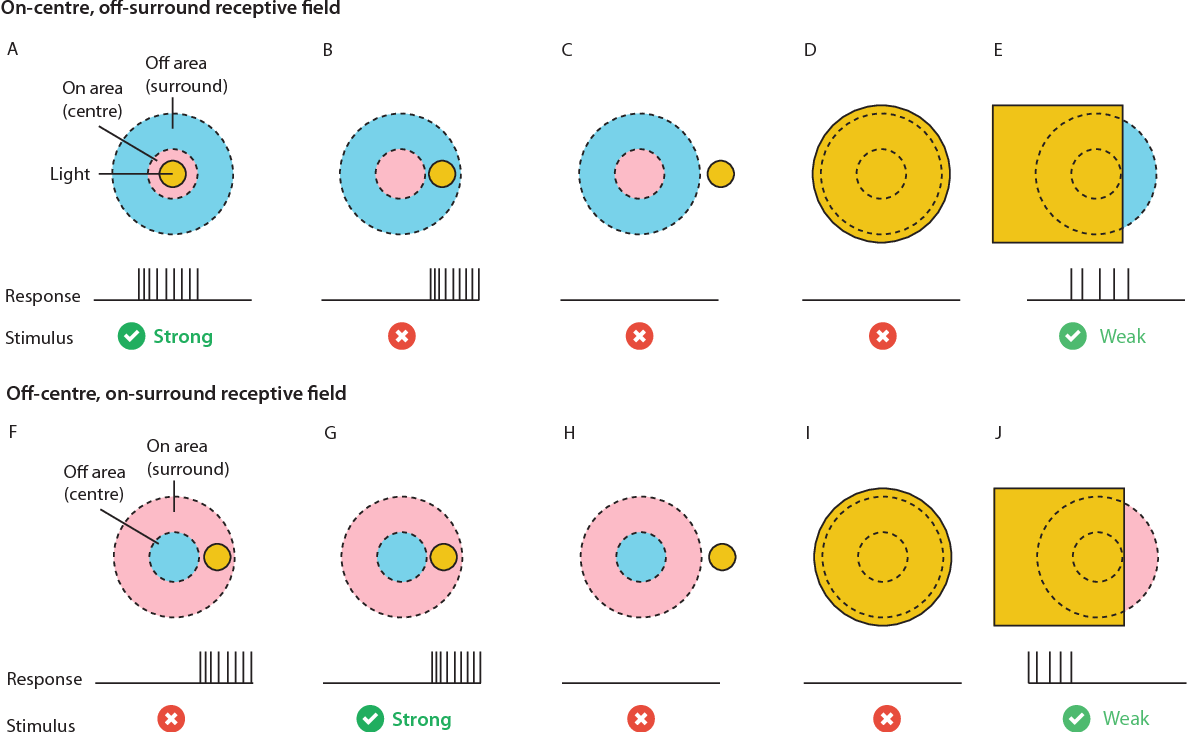
\includegraphics[width=1\textwidth]{../figures/01_33-Figure2.8-1}
    \caption[Receptive fields of retinal ganglion and LGN cells]{Receptive fields of retinal ganglion and LGN cells. Adapted from \citep{thesis_2015}.}
    \label{fig:1.1}
\end{figure}

From the eye most of the signal travels to LGN\footnote{Describing the visual pathway as a strictly feed-forward network is a great simplification.}, which serves as an active bridge to the visual cortex at the back side of the brain. Much like later V1, LGN is composed of 6 layers. The processing that happens here could be summarized as very similar to the retinal ganglion cells, only with bigger receptive fields. It is important to note that LGN does not get input only or even mainly from retina. It also receives substantial feedback from the primary visual cortex, and has synapses from parts of the thalamus and the brain stem. For example, the brain stem connection is believed to be responsible for perceived visual impacts of alertness changes, such as a flash of light when one is startled in a dark room. However, the exact role of these extra-retina sources in LGN function remains largely not understood. This means that the activity of both LGN, and all downstream stages of processing, such as V1, is modulated not only by the visual stimuli but also other neural activity inducing factors, for example emotions, locomotion, or other sensory inputs. Any models predicting the activity of LGN, V1, or higher stages of visual processing that are based solely on visual stimuli cannot, therefore, explain the entirety of recorded data. Nevertheless, under restricted experimental conditions, a wide range of studies have shown that the response of LGN cells can be very well approximated by a linear filter composed of difference-of-Gaussians. 

At last, the signal reaches the primary visual cortex. It is divided into 6 layers. Within V1, we recognize two main functional cell types - the so-called simple and complex cells. Simple cells, as their name suggests, can be represented as mostly linear combinations of ON and OFF cells. This means that within their receptive fields, they have well defined excitatory and inhibitory regions. In essence, they elicit response when stimulus, in this case light, hits the excitatory regions substantially more than the inhibitory regions. Their receptive field tends to be axis aligned, making them sensitive to oriented edges and gratings. They are also commonly described as Gabor-like filters (see Fig. \ref{fig:1.2}). 

\begin{figure}[H]
    \centering
    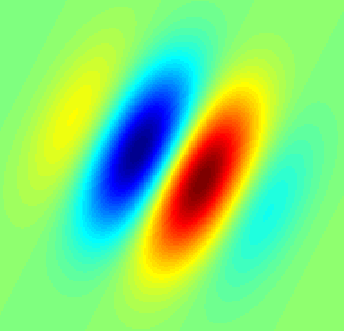
\includegraphics[width=0.2525\textwidth]{../figures/01_Gabor_filter}
    \caption[Gabor filter-type receptive field typical for a simple cell]{Gabor filter-type receptive field typical for a simple cell. Blue regions indicate inhibition, red excitation. Figure was adopted from \citep{pict_gabor_filter}.}
    \label{fig:1.2}
\end{figure}

The nature of complex cells is not yet entirely settled, but it is understood that the relationship between the visual input and their response cannot be explained with linear function. Complex cells are known to be orientation selective, just as their simple counterparts, but their hallmark is that they are not sensitive to the exact position of the oriented stimulus within their receptive field. It is thus hypothesized that their output is a non-linear combination of a number of co-oriented simple cells. If the hypothesis was true, it would essentially create a hierarchy, where the LGN cells roughly correspond to concentric ON/OFF filters of the stimuli, simple cells to a linear combination of LGN neurons, and complex cells to nonlinear combinations of simple cells. In addition to aforementioned stimuli, V1 neurons are also selective to other visual features, such as color, phase, spatial and temporal frequencies etc.

\section{Computational neuroscience}

In the following subsections, we provide an introduction to the traditional system identification methods used in visual neuroscience. For further details, refer to \textit{Data-driven approaches to understanding visual neuron activity} \citep{doi:10.1146/annurev-vision-091718-014731} or \cite{Carandini10577}'s review.

\subsection{General overview}

In computational neuroscience, we can generally distinguish two lines of inquiry. The first one, attempts to model biological reality even on the lowest level, focusing on particularities of every single neuron. Due to the inherent computational requirements of evaluating the biological neuron model, including the necessity to properly simulate temporarily to allow for mechanisms like refractory period, they usually do not scale well to larger systems. Such models are usually too complex, with too many free parameters to be fitted directly to recorded neural data through gradient based techniques. 

The second approach abstracts away details of singular neurons and focuses on higher level computation and topological properties. As such, it can leverage tools from classical machine learning and most recently even deep learning. It is prevalent in visual sensory neuroscience where it is commonly needed to model ‘black-box’ systems, such as the whole path from retina to primary visual cortex across dozens of neurons. In such models, the neural function is represented by a relatively generic computation whose parameters are fit to data to correspond to each neuron’s specific processing. Formally, for stimuli $s$, response $r$, parameters (also called weights) $o$, and model $m$, we have (Eq. \ref{eq:1.1}).

\begin{equation}\label{eq:1.1}
    r=m(s|o)
\end{equation}

In the rest of this chapter, and thesis in general, we will consider only statistical models for solving system identification tasks within the domain of visual sensory neuroscience. Our inputs will be images presented to a subject, in case of our data a mouse, in a form of 2D pixel matrices. The outputs will be real values, one per recorded neuron, representing an estimate of the measured neural activity elicited by presentation of the given image.

\subsection{Classical models}\label{ch:1.2.2}
The simplest method possible for predicting a single neuron’s response to an image stimuli is a linear model, essentially a linear regression over the pixels of the input. Mathematically, for parameters $o$ (also called weights, or in this case filter) and an image of height $h$ and width $w$ pixels that gives us the equation \ref{eq:1.2}. In such a linear model, the weights can be fitted in a number of ways, either through gradient descent methods, or analytically to compute the optimal solutions from the whole dataset. The second approach is commonly called Spike Triggered Average (STA). Both ways of fitting can incorporate regularization for the weights, for example to punish a high first derivative in both spatial dimensions, ensuring smoothness \citep{first_kernel}. This is particularly necessary in the neuroscientific settings where datasets tend to be of limited size, and overfitting of models is thus a major challenge. 

\begin{equation}\label{eq:1.2}
    r = \sum_{x,y=0}^{w,h} s_{x,y} * o_{x,y}
\end{equation}

A natural extension of a linear model is a linear-nonlinear (LN) model. As the name suggests, it is a linear model whose output is modulated by a single nonlinear function $f$ (Eq. \ref{eq:1.3}). This type of model is commonly used in a regularized variant (rLN). Due to its direct interpretability - we can easily visualise the filter, ease of analysis - the parameters (filters) are easy to compare and work with using image processing toolkit, and computational simplicity - it is just a linear operation, LN models were the de facto standard model of computational neuroscience until relatively recently.

\begin{equation}\label{eq:1.3}
    r = f(s \cdot o)
\end{equation}

In an effort to further improve the prediction power of the LN model, several of its extensions appeared. First as a generalized LN model (GLM), where one filter is replaced with a set of $k$ filters (Eq. \ref{eq:1.4}). 

\begin{equation}\label{eq:1.4}
    r = f(s \cdot o_0, s \cdot o_1, ..., s \cdot o_k)
\end{equation}

Since the k-ary non-linearity function can combine the individual results in a non-linear way, this increases the computational expressiveness of the model. There are two limitations of this approach. It makes the k-ary function an additional hyperparameter and, in turn, does not allow the way individual filters are combined to be fitted to data. The LNLN model solves both problems, replacing the k-ary non-linear function with a linear combination of several LN models (Eq. \ref{eq:1.5}):

\begin{equation}\label{eq:1.5}
    r = f(\sum_{i=0}^{k} w_i * f_i(s \cdot o_i))
\end{equation}

In addition to solving the two problems of GLM and being more interpretable, as it is simply a linear combination of LN models whose filters we can visualise with a non-linearity at the end, the fact that the combination can be individually parametrized opened the door to a particular multi-step learning strategy. When modeling multiple neurons that are believed to be similar in function, we can share the first level filters ($o_i$) between them, and only individually fit the $w$ parameters. This allows the filters $o_i$ to be based on more data - from all neurons instead of just one, and in turn, decreases the chance for overfitting.

\label{intr:hard-reg}\label{intr:soft-reg}Furthermore, the filters can be parametric, e.g. gabor functions \citep{Kay2008}, gaussians, or pre-computed bank of filters - for example borrowed from classical image processing toolkit. This can serve two goals. First, significantly decrease the number of free parameters of the model. While a normal filter for a 31x31 image has 961 parameters, a simple gaussian filter has only 4, strength, x and y coordinates of the center, and width. Second, it can ground the model in biological reality. For example, the computational properties of retinal ganglion cells are known to be well approximated in space by a difference-of-Gaussian function\footnote{A subtraction of two concentric 2D Gaussians.} and so one can inject such priors in the model. We will call this approach hard regularization. Similar effect can be achieved on arbitrary filters with regularization during parameter fitting which penalizes forms of the filter that diverge from our desired shape, as explained above for the LN model. We will call that soft regularization.

\section{ML and Deep neural networks}
In this section we will provide a brief overview of deep neural networks (DNN) fundamentals to introduce the most relevant principles and unite terminology. For a comprehensive description of general machine learning and particularly DNN methods please refer to the \textit{Deep Learning book} \citep{Goodfellow-et-al-2016}.

\subsection{Feed forward neural network}
Deep neural network (DNN) is a statistical machine learning model vaguely inspired by the brain. The term neural comes from the fact that it is traditionally composed of computational neurons\footnote{Not to be confused with biological neurons.} (also called perceptrons\footnote{\citep{Rosenblatt1958ThePA}}). Computational neurons are mathematically defined as a weighted sum of their inputs followed by, usually a non-linear, activation function. Deep and networks, because they are usually composed of several interconnected layers of neurons. A single layer of a DNN is defined by its inputs $x$ and outputs $y$ tensors. The output of the $k$-th neuron of the simplest, a fully connected, layer with $n$ inputs is then (Eq. \ref{eq:1.6}):

\begin{equation}\label{eq:1.6}
    y_k = f(\sum_{i}^{n} x_{i} * w_{k,i})
\end{equation}

When multiple layers $f_1, f_2, \dots, f_n$ are stacked on each other - to form a deep neural network, the outputs of the preceding layer are used as the inputs of the following one. The output of a complete DNN is then $y = f_n(\dots f_2(f_1(x))\dots)$. To tie this back to computational neuroscience, a LN model would be a single layer neural network. Its input size would be equal to the size of stimulus and output size to 1, as we are predicting a single neuron. Similarly, a single neuron LNLN model would be two layers DNN, where the size of the first layer would correspond to the number of LNLN filters, and the second would have size 1. If we wanted a LNLN model where the filters are shared across multiple fitted neurons, it would again be two layers DNN. The second layer would have size corresponding to the number of recorded neurons, however. Each output neuron (output of the second layer) would then be an independent combination of shared filters (the outputs of the first layer).

\begin{table}[h]
    \renewcommand{\arraystretch}{1.2}
    \centering
    \begin{tabular}{l|l}
        \toprule
        \textbf{Name} & \textbf{Function} \\ \midrule
        ReLU & $f(x) = max(0, x)$ \\ 
        Sigmoid & $f(x) = \frac{1 }{1 + e^{-x} } $ \\ 
        SoftPlus & $f(x) = ln(1+e^x)$ \\ 
        Linear/Identity & $f(x) = x$ \\ 
        TanH & $f(x) = tanh(x)$ \\ \bottomrule

    \end{tabular}
    \caption[Commonly used activation functions]{Some of the commonly used activation functions\protect\footnotemark.}
    \label{tab:1.1}
    \renewcommand{\arraystretch}{1.0}
\end{table}

\footnotetext{For neural modeling, strictly positive functions such as ReLU or SoftPlus are especially interesting due to the non-negative nature of firing rate.}

Much like the LNLN filters, DNN layers do not have to be generic. Similar to what we termed hard regularization, they can exploit known properties of the computation they are trying to model. Most notably, convolutional layers make use of local properties of inputs with continuous dimensions, such as the spatial dimensions of image inputs\footnote{Deep neural networks with convolutional layers are commonly called convolutional neural networks (CNN).}. Their outputs are the result of a location invariant filter applied at all spatial locations of the input. For more information, refer to introduction to \textit{Convolutional networks} in \cite{thesis_hojdar}.

\subsection{DNN training}\label{ch:1.3.2}

Due to the number of free parameters in even relatively shallow DNNs, these models cannot be fitted analytically. Instead, iterative gradient descent based methods, such as stochastic gradient descent (SGD \citep{kiefer1952}) or more recently ADAM \citep{kingma2014adam}, are commonly used. In gross simplification, the fitting process, also called model training, works as follows. A small random subset (batch) of input and corresponding desired output (gold data) is taken from the dataset. The input portion of a batch is used as the model’s input, computation happens, and we get a prediction (response) from the model. Then, the model’s response and corresponding gold data are put into a loss function. It serves as the metric of how far the model prediction was from the desired output. The loss function can also penalize certain properties of the model’s parameters (e.g. increase the loss for every non-zero weight). As the last step, first derivatives of the loss function with respect to all the model’s free parameters are taken (gradient) and subtracted (model update) from the parameters to, in theory, decrease the loss value next time. This step is repeated for all batches in our dataset\footnote{This means a larger batch size proportionally leads to less model updates per epoch.}. The whole process up until now constitutes one epoch. Epochs are then repeated until convergence.

In addition to layers that provide direct computation, DNNs can also feature layers whose primary objective is to help during training. One such example is the dropout layer as introduced by \cite{JMLR:v15:srivastava14a}. It randomly zeros portion of its output neurons during training, thus forcing the rest of the network to not to rely on individual inputs, and prevents overfitting\footnote{Another interpretation of the dropout layer is that it effectively trains an ensemble of models that share the majority of parameters.}. Another is the batch normalisation layer introduced by \cite{2015arXiv150203167I}, that forces its outputs to be of 0 mean and 1 variance within a single batch, and - if needed - to learn any linear transformation of its outputs explicitly. This aims to stabilise the learning process. 

\subsection{Transfer learning}
Training a DNN, e.g. for a vision task, from scratch requires large amounts of data. Fortunately, the observation that the initial layers of any DNN trained on image data are functionally similar, starting at low-level feature detection and eventually building up to higher level concepts, allows us to leverage models trained on generic tasks with huge pre-existing datasets. 

We can simply take an initial portion of an already trained network, use its layers including trained weights as the foundation of a new model, and only append it with a few new problem specific layers that are then trained from scratch. This can substantially cut down on the amount of data required, as we only need to constrain the parameters of newly added layers, and also serves as a regularization technique, making sure the initial low level filters are not overfitted on our limited data\footnote{\citep{2018arXiv180801974T}}. 

\section{DNNs and computational neuroscience}
There are several differences between system identification tasks of computational neuroscience and classical problems of computer vision. Mainly, the amount and quality of data. Where for example image classification datasets usually feature tens of thousands of precisely annotated examples\footnote{Cifar-10: \citep{cifar10}, Fashion-MNIST: \citep{xiao2017}}, system identification tasks on early visual processing have often only few thousands of substantially noisy recordings. This has vast implications for not only viable architectures, as more layers mean more free parameters (e.g. 65 millions in case of YOLOv3\footnote{\citep{2018arXiv180402767R}}) that have to be constrained by data to prevent overfitting, but - as we will see, also has the potential to invalidate our intuition around many aspects such as regularization and model stability we might have from working with larger models and datasets. 

In the following section we will introduce particular tools and techniques that are commonly used by system identification methods in neuroscience and which will be featured in our exploration, but are not as well known in the classical machine learning or computer vision domain. 

\subsection{Poisson versus Gaussian loss function}\label{ch:1.4.1}

Since our system classification problem is essentially a regression, the output consists of a real valued response for each neuron. We need an appropriate loss function to measure the distance of the model’s prediction to the recorded data. It is common to assume that the data contains noise with Gaussian distribution and then construct the loss function through most likelihood estimation (MLE) method, leading to mean squared error (MSE). Gaussian distribution is commonly used due to it being the maximum entropy probability distribution for a fixed mean and standard deviation. Intuitively speaking, it is the distribution that assumes the least given mean, which is zero for the noise, and static variance.

In our case, with outputs that are proportional to the spike rates of neurons, we do not have to assume the most generic distribution, however. There is evidence \citep{Goris2014} that the variance of neural response roughly corresponds to the neuron’s firing rate. Furthemore, spiking outputs are strictly non-negative, invalidating the assumption of Gaussian distribution. That means Poisson distribution, which assumes variance proportional to its mean and is non-negative, is a more optimal choice for modeling them. Through MLE, for measured firing rate $x$ and predicted firing rate $y$ that gives us the loss function on equation \ref{eq:1.7} .

\begin{equation}\label{eq:1.7}
    loss(x,y)=y-x\log{(y)}
\end{equation}

\subsection{Correlation as performance metric}\label{ch:1.4.2}

Even though the loss function based on Poisson noise assumption is the optimal metric to optimise during training, it is not very good for eventual analysis and comparison of different models, potentially across multiple datasets. Not only is it dependent on the assumed noise distribution, which is a technical detail of the fitting process, rather than a feature of the actual resulting fitted model, but it is also influenced by the scale of output data, and generally does not have an intuitive interpretation.

For those reasons, either the Pearson’s correlation coefficient (Eq. \ref{eq:1.8}) or the proportion of explained variance between each neuron’s model predicted output and its measured response is more commonly used instead. In this thesis, we will use Pearson’s correlation coefficient averaged across all recorded neurons for simplicity.

\begin{equation}\label{eq:1.8}
r(x, y) = \frac{{}\sum_{i=1}^{n} (x_i - \overline{x})(y_i - \overline{y})}
{\sqrt{\sum_{i=1}^{n} (x_i - \overline{x})^2(y_i - \overline{y})^2}}
\end{equation}

\subsection{Regularizations}
In addition to the wide set of traditional parameters regularizations common to all machine learning methods, such as L1 and L2, that simply punish either the size of or the number of non-zero parameters, computational neuroscience commonly uses regularizations inspired by biological plausibility. One such regularization, that will be prominent in our experiments, is Laplacian regularization, an L2 penalty on a Laplacian convolution filter. By punishing high first order derivatives in spatial dimensions, it ensures smoothness of regularized filters.

\begin{table}[h]
    \renewcommand{\arraystretch}{1.2}
    \centering
    \begin{tabular}{l|l}
        \toprule
        \textbf{Name} & \textbf{Function} \\ \midrule
        L1 & $\sum_i \abs{|w_i|}$ \\ 
        L2 & $\sum_i w_i^2$ \\ 
        Laplacian & $\sum_{x,y, i, o}(W_{:,:, i, o}*L)_{x,y}^2, \quad L=\left[\begin{smallmatrix}
0 & 1 & 0\\
1 & -4 & 1\\
0 & 1 & 0\end{smallmatrix}\right]$
 \\ \bottomrule
    \end{tabular}
    \caption[Relevant weights soft regularizations.]{Relevant weights soft regularizations.}
    \label{tab:1.2}
    \renewcommand{\arraystretch}{1.0}
\end{table}

\chapter{Key and related works}\label{ch:2}

In this chapter, we start by introducing the \cite{antolik} model, which will be the main focus of our experiments. Further, we describe a model by \cite{klidnt}, whose separable layer contribution we will also explore. To provide some background, we finish with a quick look at a few additional related works.

\section{Antolik et al. and the DoG layer}

Published in 2016, the paper \textit{Model Constrained by Visual Hierarchy Improves Prediction of Neural Responses to Natural Scenes} by \cite{antolik} introduced a three layer DNN model to fit primary visual cortex responses to image stimuli. As its main contribution, it explored incorporating biologically plausible components with traditional DNN methods. Doing so, it managed to outperform\footnote{For results refer to section \ref{ch:4.1.2}.}, at the time of writing, other state of the art methods while providing greater interpretability and requiring less free parameters.

The model (further also referred to as the HSM model) is grounded in known hierarchical properties of the early visual system in three ways. First, it assumes that LGN units can be well modeled using difference of Gaussians filters. Second, that local population of V1 neurons share inputs from a limited number of such LGN units. Third, that simple cells can be constructed as a combination of several LGN neurons and complex cells similarly from simple cells. Based on these assumptions, the model consists of 3 layers: the first represents both the retinal and LGN computation, and the second and third the two levels of V1 neurons.

\subsection{DoG layer}\label{ch:2.1.1}

Retinal and LGN computations are modeled together using a set of parallel difference-of-Gaussian filters followed by an identity activation function. In the context of the HSM model, we will call this the filter layer. The usage of difference-of-Gaussian filters significantly decreases the number of free parameters introduced by this layer while being grounded in biological reality. Instead of \texttt{input\_width}$*$\texttt{input\_height} parameters per filter of a fully connected layer, the Difference of Gaussians layer (DoG) is parametrized by only 6 per filter: weight and width of the center and surrounding Gaussians and x, y coordinates of their shared center. The published model contains 9 filters DoG layer. For input $S{x,y}$, weights $\alpha_1$ and $\alpha_2$, widths $\sigma_1$ and $\sigma_2$, and center $\mu_x$, $\mu_y$ the output of a single DoG filter is:

\begin{equation}\label{eq:2.1}
    \sum_{x,y}^{w,h} S_{x,y}
(
{\frac{\alpha_1}{ 2 \sigma_1 \pi}} * e^{\frac{(x - \mu_x)^2 + (y - \mu_y)^2}{2\sigma_1}} -
{\frac{\alpha_2}{2 (\sigma_1+\sigma_2) \pi}} * e^{\frac{(X - \mu_x)^2 + (Y - \mu_y)^2}{ 2(\sigma_1+\sigma_2) }}
)
\end{equation}

\subsection{V1 neurons}
The two levels of V1 neurons are modeled as two consecutive fully connected layers. We will call these the hidden and output layers. The output layer has the same size as the number of measured neurons. The hidden layer is proportional to the size of the output layer. In the case of the reported model, its size is 20 \% of the number of measured neurons. Both fully connected layers are followed by a SoftPlus\footnote{Refer to table \ref{tab:1.1}.} nonlinearity.

\begin{figure}[h]
    \centering
    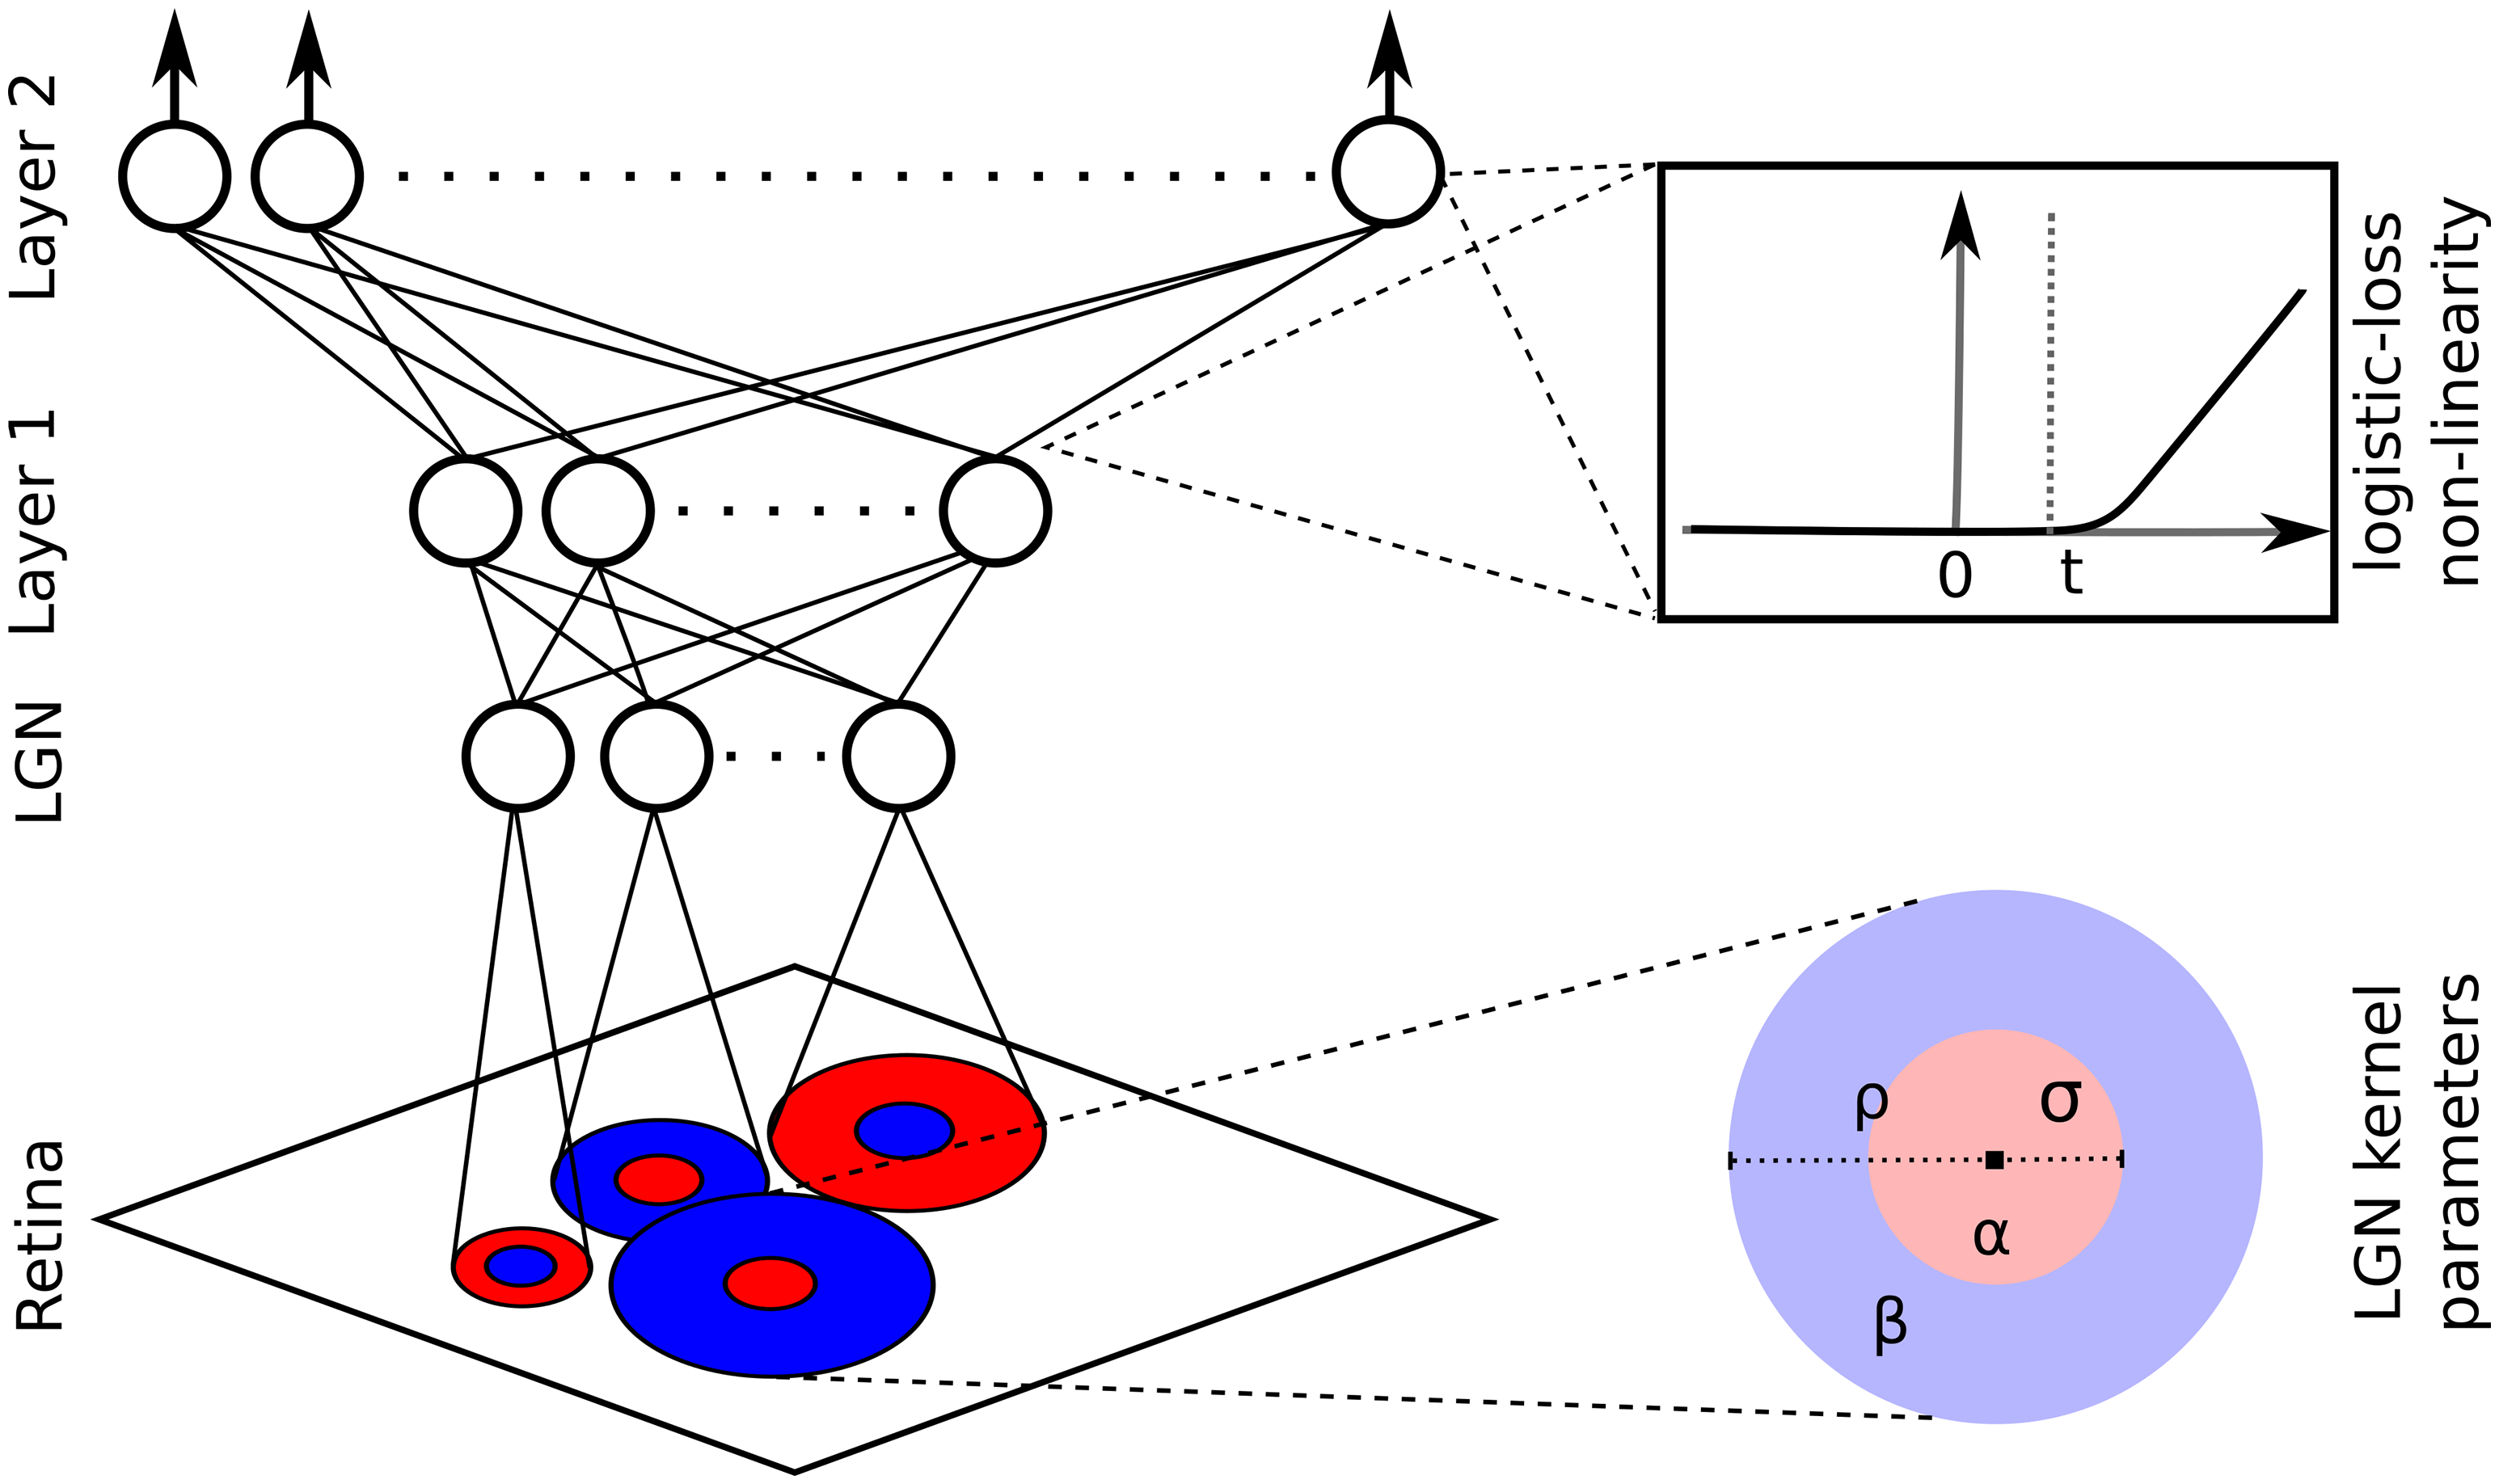
\includegraphics[width=1\textwidth]{../figures/02_HSM}
    \caption[HSM model architecture]{Three layer architecture of HSM model and corresponding neural sections. Figure was adopted from \cite{antolik}.}
    \label{fig:2.1}
\end{figure}

\subsection{Training regime}

The published model was trained using a Newton Conjugate-Gradient algorithm\footnote{\href{https://docs.scipy.org/doc/scipy/reference/generated/scipy.optimize.fmin_tnc.html}{https://docs.scipy.org/doc/scipy/reference/generated/scipy.optimize.fmin\_tnc.html}.} with 100 epochs, each consisting of 10 000 evaluations maximum. The batch size for this optimiser is the entire dataset. In addition to the hard regularization\footnote{We are referring to our definition of hard regularization (see in \hyperref[glos:hard-reg]{Glossary}).} provided by the parameterized filters of the DoG layer, all parameters - of the weights of DoG layer and both fully connected layers - were kept within predefined bounds by the optimiser throughout the fitting. These bounds were also used for random initialization of the parameters, during which values were drawn from uniform distributions with corresponding bounds. No other soft or hard regularization is present in the model. 

The reported values for the hidden layer size ratio and the number of DoG filters hyperparameters were found empirically using two one-dimensional searches through the parameter space.

\section{Klindt et al. and the separable layer}\label{ch:2.2}

In 2017 Klindt et al. published a paper \textit{Neural system identification for large populations separating “what” and “where”} (\cite{klidnt}) that explored deep convolutional neural networks in the context of V1 neural data. It specifically focused on the estimation of individual neurons’ receptive field locations through a novel approach to readout layer\footnote{Readout layer is the first fully connected layer after a set of convolutional layers.} factorization, in an effort to allow effective fitting of thousands of neurons on relatively little data simultaneously. In addition to artificial data, it was also evaluated on the same dataset as \cite{antolik} where it achieved state of the art results\footnote{For results refer to section \ref{ch:4.1.2}.}, improving on Antolik et al.

\subsection{Architecture}

The what/where model consists of two parts, feature space and receptive fields. The feature space is a cascade of - in the variant for Antolik et al. dataset - 3 convolutional layers, each followed by a batch normalisation\footnote{\cite{2015arXiv150203167I}} and a SoftPlus activation function. The convolution layers have 48 feature maps per each layer, with the first one having 13 pixel and the other two 3 pixel kernels. In addition, the convolution layers feature two types of soft regularizations. A Laplacian regularizations to ensure smoothness of the filters and an L2 based group sparsity regularization\footnote{For a definition, please refer to the original paper (\cite{klidnt}).} to encourage filters to pool from only a small set of feature maps in the previous layer.

\begin{figure}[h]
    \centering
    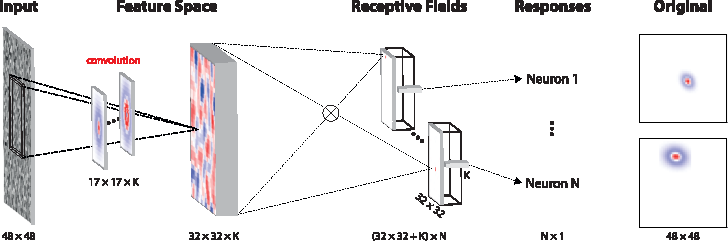
\includegraphics[width=1\textwidth]{../figures/02_fig2}
    \caption[Klidnt et al. model]{Architecture of Klindt et al. model, consisting of convolution layers and a factorized readout layer. Figure was adopted from \cite{klidnt}.}
    \label{fig:2.2}
\end{figure}

The receptive field consists of a single readout layer (further referred to as the separable layer). It is a fully connected layer factored into two masks per each output neuron. First mask, with dimensionality \texttt{feat\_space\_output\_spatial\_dims}, selects the input locations the output neuron will use, in essence its receptive field - the “where”. The other, with dimensionality of \texttt{feat\_space\_output\_channels}, determines what channels of the feature space at each of the locations will make the neuron’s output - its “what”. This factorization achieves two things. It decreases the number of free parameters, from \texttt{spatial\_dims}$*$\texttt{channels} to \texttt{spa\-tial\_dims}$+$\texttt{channels} but also enables more direct interpretability of the parameters. Comparing the “what” masks, for example, allows us to identify similar cell types. Both masks feature L1 regularization to encourage sparsity.

The model was trained using ADAM optimiser and early stopping on 20/80 training set split. Reported hyperparameters, such as the number and size of convolution filters, were found and cross-validated using grid search for each region.

\section{Related works}
To provide some background, this section lists a few related works that are relevant to V1 system identification but are not directly used or in any way referenced by our experiments. Specifically, we will introduce a few convolutional architectures, as they have seen an increase in usage for V1 modeling, similarly as they have taken over classical computer vision\footnote{Even though they are slowly being superseded by attention/transformer-based networks (\cite{2019arXiv190605909R}, \cite{2019arXiv190409925B}), \cite{dosovitskiy2020image}).}.

\subsection{Neural convolutional models}
\cite{ecker} inspired by aforementioned \cite{klidnt}, further explored convolutional architectures. In addition to the Klindt et al.’s observation that many neurons of early visual processing are similar but only have their receptive fields at different locations, Ecker et al.’s model leveraged the fact that even more V1 neurons are functionally the same, if we assume not only arbitrary receptive field positions but also arbitrary orientations. Based on the same two parts, 3 convolutional layers architecture introduced by Klindt et al., their model used Group equivariant convolutions (\cite{2016arXiv160207576C}) instead of traditional convolution layers.

Tackling a similar problem from a different angle, \cite{Walke506956} introduced a convolutional architecture, where the readout locations - representing the receptive fields of output neurons - are modulated by a shifter side network based on eye movement data. In addition, the neural outputs are further adjusted by a second side network using behaviour data (running state, pupil dilation), trying to incorporate extra-retina sources of LGN and further downstream stages of visual processing. For the core network, the model used a three layer convolutional cascade followed by a neuron specific linear readout stage. 

\subsection{Transfer learning}

Motivated by the observation that lower parts of the visual pathway can be seen analogous to early layers of classical object recognition neural networks, \cite{10.1371/journal.pcbi.1006897} explored transfer learning within the domain of V1 system identification. Their proposed architecture used 16 feature maps\footnote{The output of one filter of a convolutional layer given a specific input.} from the initial section of an on-image-classification-dataset already trained VGG-16 network (\cite{VGG16}) and then fitted per output neuron readout layer on neural data. This approach managed to achieve parity with a 3 convolutional layer CNN architecture trained entirely on neural data, while requiring a smaller training dataset.

\chapter{Implementation}\label{ch:3}
In this chapter, we are going to provide a high-level overview of the NDN3 library, introduce our extensions of it, and briefly describe the system developed for running and analysing experiments. It is intended as neither comprehensive documentation nor a detailed implementation guide. We include it to clarify the software infrastructure context of the project and to facilitate its future continuation. 

All code implemented as part of this thesis, including all experiment scripts, can be found within or is explicitly referenced by the msc-neuro github repository\footnote{\href{https://github.com/petrroll/msc-neuro}{https://github.com/petrroll/msc-neuro}}.

\section{Overview of NDN3 library}
NDN3 is a modeling framework for describing nonlinear computations in expe\-rimentally-measured neural data. It is focused on feed-forward stimulus processing but can facilitate latent variable models as well. It comes with a comprehensive set of readily available layer types, regularizations, and tools that are either biologically inspired or of particular relevance to neural data analysis. Through its TensorFlow foundations, it provides high performance and allows easy extension with new tools using state of the art machine learning primitives.

It is an ongoing project developed by the Neurotheory Lab\footnote{\href{http://neurotheory.umd.edu/}{http://neurotheory.umd.edu/}} of prof. Dan Butts\footnote{\href{http://biology.umd.edu/daniel-butts.html}{http://biology.umd.edu/daniel-butts.html}} at the University of Maryland. It started as a python2 library FFNetwork in late 2017 and was soon transformed into a comprehensive NDN framework in early 2018. In 2019 work on its port to python3 in the form of NDN3\footnote{\href{https://github.com/NeuroTheoryUMD/NDN3}{https://github.com/NeuroTheoryUMD/NDN3}} began. Recently, following prior collaboration, it has been adopted by Jan Antolik’s group at the Faculty of Mathematics and Physics of Charles University. 

Under the hood, NDN3 is implemented using TensorFlow 1.x (TF)\footnote{\href{https://www.tensorflow.org/}{https://www.tensorflow.org/}}, NumPy (NP)\footnote{\href{https://numpy.org/}{https://numpy.org/}}, and a few other libraries from the SciPy stack. Its intended usage philosophy is similar to TensorFlow 2.x sequential approach\footnote{\href{https://www.tensorflow.org/guide/keras/sequential_model}{https://www.tensorflow.org/guide/keras/sequential\_model}}. The centerpiece is an object-oriented model instance whose architecture is defined using a list of layer types and parameters as they sequentially form the model.

At the highest level, there is an instance of an NDN model class. The NDN instance encapsulates the complete computational model, its architecture, hyperparameters, trained weights, etc. For manipulation, it provides methods for fitting to data, accuracy evaluation, or generating new predictions based on provided stimuli. It can also serialize and save itself to a file or load itself from one. 

On creation, NDN model’s constructor receives a list of dictionaries, each describing a network that will be part of the model (Fig. \ref{fig:3.1}). For our experiments, we will limit ourselves to just one network per model but NDN3 allows multiple in various configurations, such as side networks and sampler networks. Each network is a feed-forward stack of layers. It is fully described by a dictionary of number-of-layers-long lists where every key represents a parameter and its value - in the form of a list - dictates what the value of that parameter should be for each layer of that specific network.

\begin{figure}[h]
    \centering
    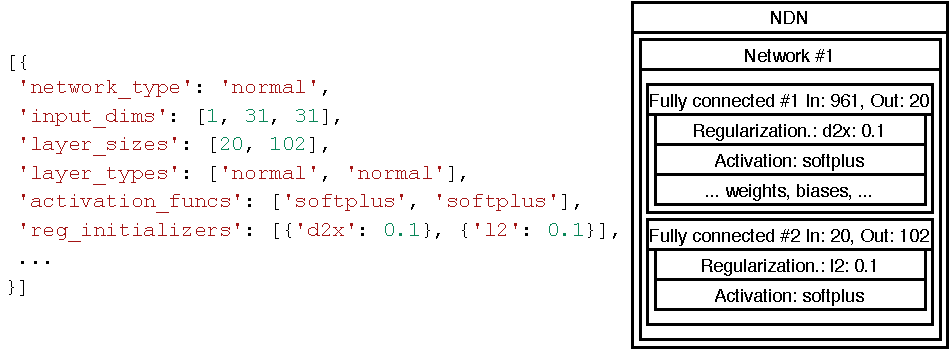
\includegraphics[width=1\textwidth]{../figures/03_NDN_1}
    \caption[NDN model description and subsequent architecture]{Model description and the resulting NDN instance for an LNLN model with 31x31 pixels input, 102 output neurons, 20 filters, softplus non-linearities, and regularizations.}
    \label{fig:3.1}
\end{figure}

The NDN model class recursively contains instances representing its parts. The NDN object includes an array of network objects, each network object contains a stack of layer objects, and each layer object has, among others, regularization objects. The layer object also contains fields representing all of its hyperparameters, specifying its activation function, and - among a few more - also maintains NP arrays backing all its free parameters such as weights and biases. All of this structure is created as part of the network's definition which happens from within the NDN’s constructor. This is also where parameters initialization happens through the backing NP arrays.

Whenever computation is invoked - e.g. when \texttt{train} or \texttt{generate\_predic\-tion} methods are called, a new TF session is initialized, a computational graph is recursively created from scratch using the description saved on the internal network and layer objects, and finally, weights are loaded to the session from the aforementioned layers’ parameters backing NP arrays. When the computation finishes, all weights are gathered from the TF session to plain NP arrays and saved within layers’ objects of the model again. For visualisation, refer to figure \ref{fig:3.2}.

\begin{figure}[ht]
    \centering
    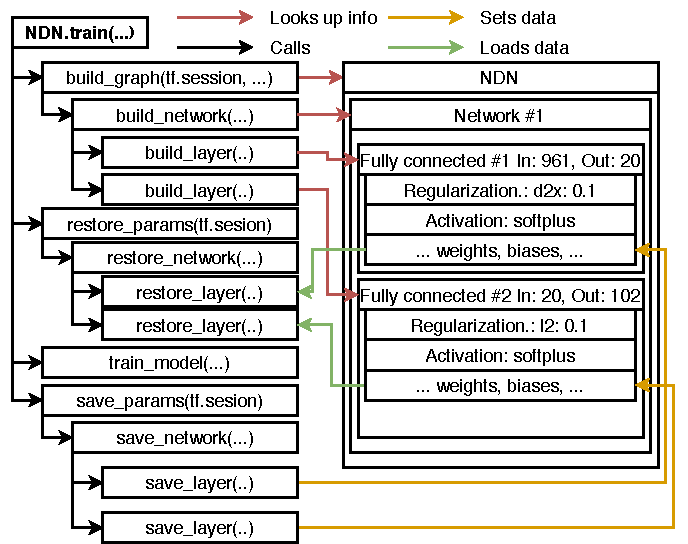
\includegraphics[]{../figures/03_NDN_2}
    \caption[NDN computation graph initialization]{Diagram of NDN model initialization when \texttt{train(...)} method is called.}
    \label{fig:3.2}
\end{figure}

All shapes are inferred from input dimensions, specified layer sizes, and - e.g. in the case of convolutional layer - its stride and filter size, with the last layer size serving as the output dimensions. The interpretation of input dimensions is (\texttt{time}\footnote{This is to support temporal models which we will not cover.}, \texttt{width}, \texttt{height}). Internally, the framework assumes \texttt{(batch\_shape, height, width, channels} or \texttt{time)} dimensionality and uses flatten representation to float data between layers. When necessary, for example to apply 2D convolution, a layer restores the full dimensionality, both spatial and channels/time dimensions, and, after applying its function, flattens the data again. 

\subsection{NDN3 toolkit}\label{ch:3.1.1}

The featureset of NDN3 is vast and continuously evolving and so it is not our intention to provide a comprehensive summary. Below is just a subset of tools that are either relevant to our work (implemented additions in italic) or that we wanted to particularly draw attention to for potential future continuation of our exploration.

\begin{itemize}
    \item \textbf{Loss functions (noise assumptions):} Gaussian, Poisson, Bernoulli.
    
    \item \textbf{Layers:} Fully connected (normal), Separable, Convolution, Convolutional separable\footnote{Each filter is factored into a convolutional what and where masks.}, Readout\footnote{Outputs the value of spatial location defined by an explicit parameter. Not to be confused with general readout layer as defined before.}, Convolutional readout, Additive\footnote{Combines inputs from multiple input streams.}, \textit{DoG}, \textit{Convolutional DoG}, \textit{Linear scale}\footnote{Linearly scales its input using a scalar multiplier and single additive bias: $input*x + b$.}, etc.
    
    \item \textbf{Parameters regularizations\footnote{Regularizations are the only externally documented part of NDN: \href{https://github.com/NeuroTheoryUMD/NDN/blob/master/docs/glossary.rst}{https://github.com{\-}/NeuroTheoryUMD/NDN/blob/master/docs/glossary.rst}}:} Dropout, center\footnote{Penalizes higher weights far from the center.}, norm2\footnote{Encourages norm of weight matrix to be 1.}, max\footnote{Penalizes more than 1 non-zero weight, both in spatial and channel dimensions.}, L1, L2, Spatial Laplacian (d2x), etc.
    
    \item \textbf{Parameters normalizations\footnote{This is parameters normalization I.e weights are normalised each time before used. Activation normalization, such as batch normalisation (\cite{2015arXiv150203167I}), is notably missing.}:} maxnorm, L2.
    
    \item \textbf{Activation functions:} ReLU, sigmoid, tanh, identity, SoftPlus, leaky ReLU, etc.
    
    \item \textbf{Weights/bias initializers:} zeroes, normal\footnote{Normal distribution with 0 mean, 0.1 variance.}, trunc normal\footnote{Absolute value of normal.}.
\end{itemize}

Apart from these traditional tools, NDN3 also provides following capabilities:

\begin{itemize}
    \item \textbf{Metrics capture:} Loss value and \textit{potentially\footnote{Not merged upstream, please refer to the msc-neuro's readme.} correlation metrics} can be logged as TF summaries periodically throughout the training loop as part of the summary step.
    
    \item \textbf{Layer activation logging:}  In addition to model-wide metrics such as the loss value, NDN3 allows for individual layers’ activations to be logged as histograms.
    
    \item \textbf{Validation while training:} If specified, a validation set can be evaluated using abovementioned metrics as part of the summary step of the training loop every few epochs. Do note that the validation set is evaluated in its entirety at once and is not batched. Respective metrics are saved as a separate TF summary.
    
    \item \textbf{Support for early stopping:} Using the same mechanism as the abovementioned validation metrics, NDN3 supports early stopping.
    
    \item \textbf{Explicit inhibitory/excitatory neurons enforcement:} It is possible to specify the ratio of excitatory/inhibitory neurons on supported layer types (normal, convolution, etc.). This works through enforcing strictly non-negative weights and then multiplying the layer’s output with a +/-1 mask.
    
    \item \textbf{Data filters:} In addition to input and output data, it is possible to provide data filters. A boolean mask of the same dimensionality as the output data that specifies which individual output neurons should be ignored (zeroed for prediction, ignored for loss value computation, metrics, etc.) for what particular data points. This allows for, among other things, a common model trained on two separate recordings (e.g. 10 and 15 data examples) of two neuron regions (e.g. containing 5 and 7 neurons). The output dimensionality of such a model would be 12. Where valid output data are not available, i.e. for neurons 5 to 12 of the first 10 data points, zeroes can be used. In such case, the data filter mask has ones on the indexes 0 to 5 for the first 10 data points, and zeros for indexes 5 to 12. The situation is mirrored for data points 10 to 25. This way, when NDN model computes an output of a second region’s neuron (e.g. neuron 11) for a first region’s data point (e.g. 5th data instance) while training, it can see the 0 in \texttt{data\_filters[5][11]} mask and know to not include its not-trained output in the loss function computation and subsequent optimisation.
    
    \item \textbf{Many more:} Several data ingestion pipelines, support for temporal models, etc.
\end{itemize}

\section{Implemented NDN3 extensions}

To facilitate our research, we implemented several extensions to the NDN3 framework\footnote{Most additions were merged upstream but some remain only in a fork. For more information, please refer to msc-neuro's readme.}. Our main contribution was in the form of the Difference of Gaussians layer (for description refer to section \ref{ch:2.1.1}) as introduced by \cite{antolik}. We also implemented a convolutional variant of this layer. To help with training progression interpretability, support for Pearson’s correlation tracking as part of TF summary was also added, as well as several general fixes and other smaller-scale contributions.

The Difference of Gaussians (DoG) layer is implemented similarly to a fully connected layer, with two main differences. Instead of input dimensions worth of weights per each output neuron, it only has 6\footnote{It actually reserves 8 to support not-concentric difference-of-Gaussians filters. Such behavior is off by default but can be enabled through \texttt{impl\_concentric} parameter.}. And instead of using these weights directly, only reshaped, to multiply the input with, they are used to create a full difference-of-Gaussians filter first. Namely, they are separated into the shared center x, y coordinates, and weights and diameters parameters for each of the Gaussians. Then, the full gaussian filter is computed\footnote{This is likely not the most efficient implementation but given the size of our data and other bottlenecks within the system it never showed to be an issue.} with dimensionality of \texttt{(input\_width, input\_height, 1, number\_of\_channels)}, element-wise multiplied with the layer’s input, and spatially sum-reduced, creating a \texttt{number\_of\_channels}-wide output tensor. The output is then normally processed through activation function, bias, dropout, etc.

The convolutional variant works similarly, the only two differences being the size of the difference-of-Gaussians filter and its application. The filter is of size \texttt{conv\_filter\_widths} and, rather than being pointwise multiplied with the input, it is applied at all of its spatial locations as per the semantics of conv2D operation\footnote{\href{https://www.tensorflow.org/api_docs/python/tf/nn/conv2d}{https://www.tensorflow.org/api\_docs/python/tf/nn/conv2d}}. The same as a classical convolutional layer, it supports convolution stride and dilations. The \texttt{SAME} option is used for padding. 

Unlike the weights of fully connected and convolutional layers or their direct derivatives, the weights of either classical or convolutional variant of DoG cannot be initialized using the mechanisms already provided by NDN3 (see section \ref{ch:3.1.1}). Namely, the Gaussians center(s) needs to fit within the spatial boundaries of the input/convolutional filter, and the width should at least be proportional to the spatial dimensionality. Given that, we opted for replicating the exact initialization scheme of Antolik et al., drawing the DoG parameters from a uniform distribution with bounds proportional to the input/convolution filter size. Namely, the weights are strictly positive, widths are bounded by 1 pixel and 82 \% of the maximum of input/filter width and height, and the center cannot be closer to an edge than two pixels. 

The correlation tracking is implemented as part of the loss function evaluation. It is computed for each output neuron separately and then averaged. Several options are available: interpreting neurons’ NaN correlations as 0, ignoring NaN correlations, and - inspired by \cite{ecker} - also ignoring correlations for neurons with small variation in the recorded data. All of our experiments use the \texttt{treat NaNs as zeroes} option. The correlation tracking respects data filters (see NDN toolkit) if set, properly ignoring outputs of masked neurons.

\section{Experiments and analysis pipeline}

To enable scalable execution and evaluation of a large number of architectures implemented using NDN3, including the capability for efficient hyperparameter search, we also created\footnote{The code is hosted together with all experiments at msc-neuro.} an experiments and evaluation pipeline. It consists of three parts, experiment execution pipeline, results and analysis tools, and general NDN3 utils.

The experiment execution pipeline works as follows. For each experiment, two python scripts exist, a runner and the experiment itself. The runner iterates over all hyperparameter combinations the experiment is supposed to test and calls the experiment script with each of the combinations as command-line arguments. It does not call it directly, however, but through a backend-specific runner. The one to be used is user-selected when the runner script is invoked. Currently, five backends are implemented, one for a custom Docker-based\footnote{https://www.docker.com/} environment, two for qsub\footnote{https://en.wikipedia.org/wiki/Qsub} based systems - CPU and GPU version, and two for plain virtenv python environments on windows or linux. For each of them, separate experiment script invocations are either submitted as individual jobs or are natively run in parallel. All of them redirect standard output and standard error to by-convention-standardized log files.

\begin{figure}[ht]
    \centering
    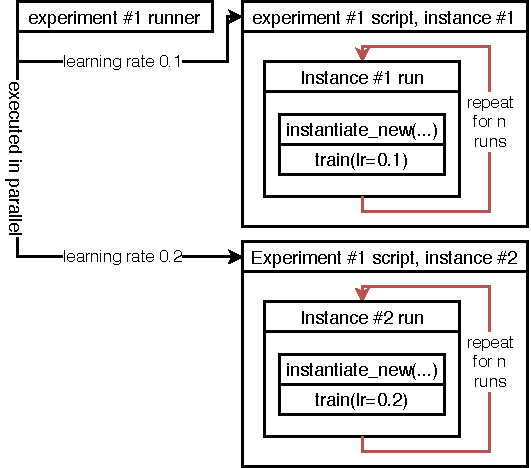
\includegraphics[]{../figures/03_msc-neuro_1}
    \caption[Experiments pipeline]{Experiments pipeline: Execution order when an \texttt{experiment \#1} with two instances (learning rate 0.1 and 0.2) is run through a runner.}
    \label{fig:3.3}
\end{figure}

The experiment script can be arbitrary, but - by convention - contains instantiation and training of a specific model architecture given a particular set of (hyper)parameters (further referred to as the \textit{experiment instance}) passed as command-line arguments, usually by the corresponding runner. As further explained in section \ref{ch:4.2.1}, each model instance is actually instantiated and trained multiple times (further referred to as the \textit{experiment instance run}) to control for the influence of random initialization. Currently, for all implemented experiments individual instance runs are executed sequentially by the respective experiment scripts. For illustration, refer to figure \ref{fig:3.3}.

Having multiple runs of, apart from random initialization, identical models presents a challenge for analysis. Instead of comparing performance of individual runs, sets of multiple runs need to be considered. To facilitate that, an analysis toolkit was created. A user can specify a list of experiment instances to be compared against each other as an array of root folders with TF summaries and filter regexes. Based on that, all relevant TF summaries of each experiment instance are gathered. For each instance, metrics are first read from the summaries files of all runs, then the values grouped by epoch number (step), and finally a few general statistics, such as deciles of performance, are computed across each instance’s individual runs. As the last step, the results are presented either as a graph (see figure \ref{fig:3.4}) - showing the metric percentiles of each instance in time, or as a summary table - representing the final trained performance. 

\begin{figure}[ht]
    \centering
    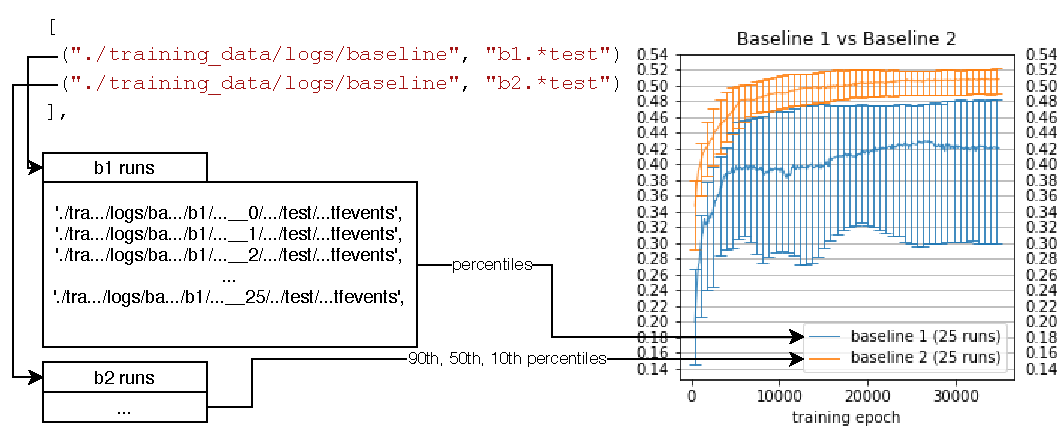
\includegraphics[width=1\textwidth]{../figures/03_msc-neuro_2}
    \caption[Experiment analysis toolkit]{Experiment analysis toolkit: Retrieval of summaries for individual runs of two experiment instances (\texttt{b1}, \texttt{b2}).}
    \label{fig:3.4}
\end{figure}

For more information about the specifics, such as the expected filesystem layout of the experiments pipeline or the exact API of analysis toolkit, please consult either the msc-neuro’s readme or the documentation that is part of respective methods’ source code. 

\chapter{Methodology}\label{ch:4}

In this chapter, we are first going to introduce our problem at hand - including an overview of the dataset we are going to be working with, then describe the methodologies of our architecture exploration process and results analysis, and finish with a section about our model training regime.

\section{The system identification task}

We are going to work with data recorded by \cite{antolik} in mouse primary visual cortex, trying to capture the computation of retinal ganglion cells, LGN, and both simple and complex cells of V1.

\begin{itemize}
	
	\item\textbf{Stimuli:} Static images of natural scenes, such as landscapes, animals, or humans, from David Attenborough’s BBC documentary Life of Mammals. The images were presented to sedated mice in 256 luminance steps grayscale and downscaled to 384x208 pixels.
	
	\item\textbf{Recorded response:} The estimated average number of spikes of a neuron in a specific time window after an image stimulus presentation. Recorded by calcium imaging method and further processed by spike extraction algorithm\footnote{The response is actually not a spike count but a variable directly proportional to it.}. In our case, a whole population of tens of neurons within a small region of V1 was simultaneously recorded for each stimulus.
	
\end{itemize}

The fact that we are working with natural stimuli is important. While the function of V1 neurons, especially simple cells, is relatively known for artificial stimuli such as white noise or small contrast lines of various orientations, the computation of complex cells on natural stimuli, containing all sorts of high and low frequency details and cross correlations, is still an open question. This is a direct consequence of the nature of simple and complex cells as intruded in section \ref{ch:1.1.1}. 

Due to the functional organization of mammalian V1, neurons recorded in a local area of visual cortex all have receptive fields within a restricted region of their visual space. Thus, there is no reason to use the entire stimulus image for response modeling. Instead, receptive fields of individual recorded neurons were estimated using a rLN model on the full stimulus and combined to form a region of interest. To account for inaccuracies, this region spanned roughly two times the area of the union of individual neurons’ estimated receptive fields. Lastly, only these regions of interest were cut out of the stimuli pictures, downscaled to 31x31 pixels, and used to form our dataset’s inputs.

\subsection{Dataset}\label{ch:4.1.1}

The dataset consists of three regions, each recorded separately, targeting different neurons, and with an individual set of stimuli. The regions contain 103, 55, and 102 recorded neurons respectively. Each region consists of a training set, with stimuli each presented only once, as well as an explicit validation set (also referred to as the test set), where each stimulus was presented 10, 8, and 12 times respectively and the responses were averaged. The training sets contain 1800, 1260, and 1800 images for the three regions while each validation set is 50 images regardless of region. Regions 1 and 2 were recorded in one animal and region 3 with another.

\begin{table}[h]
    \renewcommand{\arraystretch}{1.0}
    \centering
    \begin{tabular}{l|l|l|l}
        \toprule
        & \textbf{Region 1} & \textbf{Region 2} & \textbf{Region 3} \\ \midrule
        Recorded neurons & 103 & 55 & 102 \\ 
        Training stimuli & 1800 & 1260 & 1800 \\ 
        Training repetitions & 1 & 1 & 1 \\ 
        Validation stimuli & 50 & 50 & 50 \\ 
        Validation repetitions & 10 & 8 & 12 \\ 
        Animal & A & A & B \\ \bottomrule

    \end{tabular}
    \caption[Regions of dataset]{Summary of regions within the dataset.}
    \label{tab:4.1}
    \renewcommand{\arraystretch}{1.0}
\end{table}

The fact that the validation sets are averaged across multiple stimulus presentations while the training set is recorded only once has consequences in terms of the measured responses’ signal to noise ratio. To illustrate this: the average correlation between predicted and measured responses across region 1 neurons, as reported by \cite{antolik}, was between\footnote{Depending on random initialization.} 0.28 and 0.35 on the training set and between 0.41 and 0.52 on the validation set for the same models. Similarly for the other two regions, the performance on their validation sets was substantially higher than for the training sets. 

The stimuli, representing 31x31 pixel 8-bit grayscale images, are stored as float64 numpy arrays of appropriate dimensionality. Inexplicably, the range of pixel values is 0-0.000255 instead of the expected 0-255. For each stimulus, the measured response is a recorded-neurons-wide floating point vector representing variables each proportional to a measured neuron’s spike rate. They are stored as a float64 numpy array of respective dimensionality. The responses have a range of roughly 0-10.

\subsection{Prior work results}\label{ch:4.1.2}

Both \cite{antolik} and \cite{klindt} published results of several models on the Antolik et al. dataset as part of their papers. Table \ref{tab:4.2} shows a subset of models and their reported validation set correlations that will either be referenced later or we deem relevant for the context they provide.

\begin{table}[ht]
    \renewcommand{\arraystretch}{1.0}
    \centering
    \begin{tabular}{l|l|l|l|l}
        \toprule
        \textbf{Model} & \textbf{1} & \textbf{2} & \textbf{3} & \textbf{Paper} \\ \midrule
        HSM & 0.51 & 0.43 & 0.46 & \citeauthor{antolik} \\ 
        rLN & 0.51 & 0.43 & 0.46 & \citeauthor{antolik} \\ 
        What/Where & 0.51 & 0.43 & 0.46 & \citeauthor{antolik} \\ 
        What/Where: fully-connected readout & 0.51 & 0.43 & 0.46 & \citeauthor{klindt} \\ 
        Linear-nonlinear Poisson (LNP) & 0.51 & 0.43 & 0.46 & \citeauthor{klindt} \\ \bottomrule
    \end{tabular}
    \caption[Performance of prior works.]{Validation set correlation of prior works models on all three dataset’s regions.}
    \label{tab:4.2}
    \renewcommand{\arraystretch}{1.0}
\end{table}

Since much of our analysis is focused on stability of model performance with respect to random initialization, table \ref{tab:4.3} provides validation set correlations of 50th, 10th, and 90th percentiles\footnote{For the rationale behind using (these) percentiles, please refer to section \ref{ch:4.3.1}.} across 100 separate fittings using different initial conditions of the HSM model, as reported by Antolik et al. Regrettably, similar data are not available for Klindt et al. model or any other of the aforementioned models.

\begin{table}[ht]
    \renewcommand{\arraystretch}{1.0}
    \centering
    \begin{tabular}{l|l|l|l}
        \toprule
        & \textbf{50th} & \textbf{90th} & \textbf{10th} \\ \midrule
        Region 1 & 0.479 & 0.501 & 0.442 \\ 
        Region 2 & 0.412 & 0.435 & 0.382 \\ 
        Region 3 & 0.437 & 0.449 & 0.419 \\ \bottomrule

    \end{tabular}
    \caption[Performance percentiles of HSM model]{Percentiles of validation set correlations of HSM model across 100 different random initializations.}
    \label{tab:4.3}
    \renewcommand{\arraystretch}{1.0}
\end{table}

\section{Experiments}\label{ch:4.2.1}

Due to the size of both hyperparameters and especially architecture space, a complete exploration that would cover all possible combinations of a model for our dataset is not possible. It is not feasible even if we assume starting off a preexisting architecture, in our case the HSM model by \cite{antolik}, and would only want to explore its close neighborhood - architecture and hyperparameter wise. 

Instead of trying all combinations, we opted for the following approach. We start with a working model called and call it \textit{baseline}\footnote{The first baseline will be a reimplementation of the HSM model by \cite{antolik}}. With it as a base, we conduct a set of smaller exhaustive grid search experiments, each focused on a small set of hyperparameters or architecture aspects. After analysing these experiments, we combine the modifications that worked best and assess the performance of this new baseline model. This step is important to verify the additivity of separately tested improvements. If the new baseline model candidate performs better than the current one, it becomes the new baseline. After that, the cycle repeats with a new set of experiments. For future reference, the term \textit{experiment} refers to a single focused grid-search exploration and \textit{experiment instance} to one particular model with a specific set of hyperparameters that is, among others, assessed as part of an experiment.

Contrary to the classical deep learning assumption (\citep{2017arXiv170610239W}) that modern optimization techniques on real-world datasets should converge to reasonably similar levels of performance and generalization across multiple random initializations, Antolik et al described a substantial variance (see section \ref{ch:4.1.2}) for different initializations and subsequent training of the same model. To control for this phenomenon, all our experiment instances are run multiple times, each time with a different random seed (further referred to as \textit{experiment instance run}). To facilitate repeatability\footnote{It is important to note that TF and thus NDN3 is not entirely deterministic. For more information, refer to: \href{https://github.com/NVIDIA/framework-determinism}{https://github.com/NVIDIA/framework-determinism}.}, consecutive seeds starting at 0 are used.

\begin{figure}[ht]
    \centering
    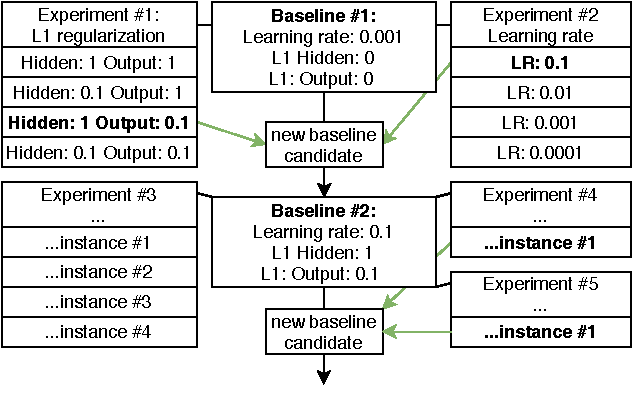
\includegraphics[]{../figures/04_explor_1}
    \caption[Experiments methodology]{Experiments methodology: Bold instances represent better performance than respective baseline models. Black lines show what baseline model was used for an experiment. Green arrows show improvements of best instances selected to form a new baseline candidate.}
    \label{fig:4.1}
\end{figure}

\begin{enumerate}[noitemsep]
    \item \texttt{Assess the performance of a baseline model.}
    \item \texttt{Run a set of experiments, each testing a modification of the\\ baseline model.}
    \begin{enumerate}[nosep]
        \item \texttt{Grid search experiment instances to cover all parameters\\ of the change.}
        \begin{enumerate}[nosep]
            \item \texttt{Execute multiple runs of each experiment instance.}
        \end{enumerate}
    \end{enumerate}
    \item \texttt{Take experiment instances that worked best and performed\\ better than baseline, combine them to a new model.}
    \item \texttt{Verify the new model is better than the old baseline. If it\\ is, make it a new baseline.}
    \item \texttt{Repeat, go to 2.}
\end{enumerate}
\begin{center}
    {The experiment exploration algorithm.}
\end{center}

The same seeds are used across both different experiments and different experiment instances. Therefore, all other things equal, the first run of instance 1 of experiment 1 has the same seed as the first run of instance 2 of experiment 1 or the first run of instance 1 of experiment 2. Due to that, runs of the same architecture differing only by hyperparameters that do not influence the number or order of randomly initialized parameters should be initialized with the same values.

Instead of this approach, we could have chosen to use either a fully automated or at least partially computer assisted method to search the model space, for example through evolutionary algorithms (\citep{2017arXiv170300548M}), Bayesian optimization (\citep{thesis_arnold}), or deep learning based autoML system (\citep{2016arXiv161101578Z}). That would, however, go against our goal to test specific modifications to Antolik et al’s model and carefully mix it with and compare to elements from traditional DNN toolkit. A comparison between our work and a more automated approach would be an interesting topic for further research but is outside of the scope of this thesis.

\section{Analysis}\label{ch:4.3.1}

As explained in the section \ref{ch:4.2.1}, when assessing two model instances we are not comparing two runs, one per each instance, but two distributions of runs. That complicates analysis as we cannot simply say that instance A is better than instance B because it achieves a higher performance metric, Pearson’s correlation in our case\footnote{For reasoning refer to section \ref{ch:1.4.2}.}, on the validation set at the end of training. Instead, we have to decide what is the representative sample out of the two distributions of runs to compare. Further, we also have to consider the variance across multiple runs, as it represents the stability of the model with respect to random initialization - an aspect we set out to explore. A model that has slightly better e.g. 90th percentile run but has two times as large variance between runs - leading to significantly worse 10th percentile, than the baseline model is neither clearly better nor worse, but is noteworthy. 

Thus, with a few exceptions, we report three metrics per experiment instance. The median correlation on validation set, 90th and 10th percentiles. We chose to report these to present a clear picture of how big of a spread individual models have depending on random initialization. Together with the higher number of runs per each experiment instance, it also makes reasonably sure we do not present random outliers while showcasing the full potential. Unlike variance, percentiles allow for accurate representation of non-symmetrical variances\footnote{E.g. when half of the runs have good performance and the other does not train at all. In that case, the 50th and 90th percentiles would be close to each other - showcasing the potential, and the 10th would be near zero correlation.} and directly show what exact level of performance the model instance is capable of.

It is important to note that each run is not represented by just a single scalar - its performance at the end of training, but a time series that shows the progress during training. For simplification, we will mostly consider only either the end of training or peak value, however. When relevant, we will draw explicit attention to the speed of convergence or other phenomena apparent only when the whole training in time is considered.

\section{Training regime}\label{ch:4.4}

We opted for a simple static and fully predetermined amount of training epochs. The reason why we did not choose early stopping instead is threefold. First, it is the simpler solution without additional hyperparameters and implementational complexity. Second, we only have limited data that is already explicitly divided into train and validation sets. Splitting either to form a test set to evaluate early stopping on might compromise either training or validation due to insufficient data. Third, due to the size of the validation set, we evaluate it fully throughout the training process, capturing all relevant performance metrics (see section \ref{ch:3.1.1}). Thanks to that, we always have the full information about the model’s peak performance on the validation set, even if we overfit after achieving it. This leaves computational efficiency as the only benefit of early stopping, which in our opinion did not outweigh the negatives\footnote{\cite{klindt} report using early stopping with a training set split of 80/20 (see section \ref{ch:2.2})}.

Based on early tests, we chose to train experiments for 5 000 epochs and baseline models for 35 000 epochs. This proved to be more than enough for experiment instances to show potential - if there was any, and for baseline models to achieve peak performance and - in case they were susceptible to it - overfit, with plenty headroom especially for later models. 

In regards to the number of runs per model instance, we have chosen 10 runs for experiment instances and 25 runs for baseline model instances to balance computational resources and statistical significance of the results. The effect of potentially higher numbers of runs on one of the least stable baseline models can be seen on figure \ref{fig:4.2}.

Unless explicitly mentioned, all of our experiments are evaluated only on region 1. Region 1 was chosen due to being the largest, highest performing, and least stable of the three regions - as reported by Antolik et al. In section \ref{ch:5.3.2} we evaluate the main architectures explored and fine-tuned on region 1 on regions 2 and 3 as well.

\begin{figure}[H]
    \centering
    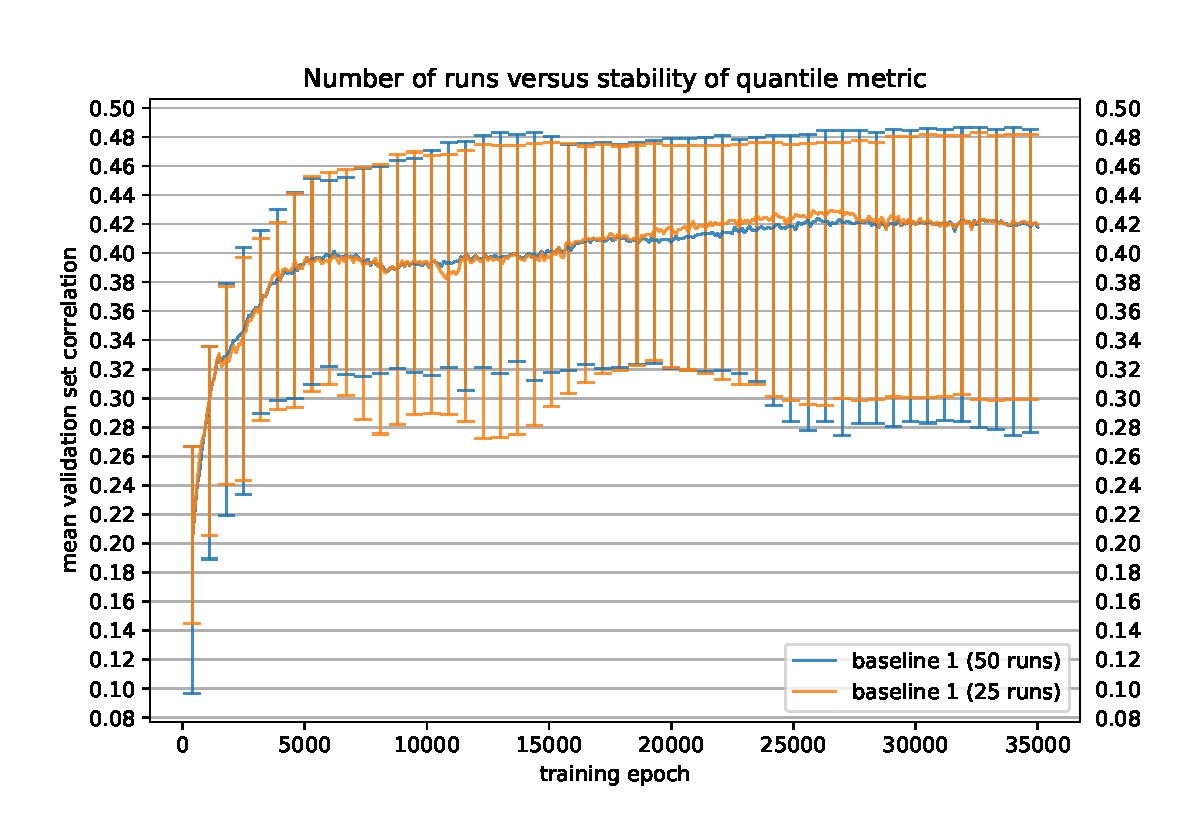
\includegraphics[width=1\textwidth]{../figures/04_runs_number}
    \caption[Impact of 25 vs 50 runs]{Illustrates the difference between running the least stable baseline model 25 and 50 times. The line represents median run, top and bottom error bars 90th and 10th percentile runs.}
    \label{fig:4.2}
\end{figure}

\renewcommand*\thesubsubsection{\arabic{section}.\arabic{subsection}.\arabic{subsubsection}}
\setlength{\abovecaptionskip}{0pt plus 0pt minus 0pt} % Chosen fairly arbitrarily

\chapter{Experiments and results}\label{ch:5}

In this chapter, we will go through all notable\footnote{We only present a subset of conducted experiments that are implemented in the \refattachment{at:msc-neuro}. Further, the experiments are reordered and their naming scheme does not directly correspond between the repository and the text of this thesis. For matching, refer to \texttt{msc-neuro/experiments/readme.txt}. Similarly, we only provide a subset of figures.} experiments and their results. It is divided into three sections. First, we focus on reimplementing, assessing, and improving the \textit{HSM model} by \cite{antolik} Second, we compare its DoG layer contribution with various less constrained variants from classical deep learning and also assess the separable layer introduced by \cite{klindt}. Lastly, we explore pooling the three regions of our dataset together for a single shared model as well as test the best architectures on each of the regions separately.


\section{Assessment and improvements of HSM}

In this section, we start by listing the differences between the original \textit{HSM model} by \citeauthor{antolik} and our reimplementation. Then, we move towards experiments focused on the effects of training regime hyperparameters on both best achieved performance and also model stability. We finish with an initial look at \textit{soft regularizations} and additional non-linearity.

\addtocounter{subsection}{-1} % Make differences 0 so that experiments start from 1.1.1 %
\subsection{Differences introduced by reimplementation}\label{ch:5.1.0}

We started by reimplementing the \textit{HSM model} by \citeauthor{antolik} Due to the differences between the tools available in the general-purpose deep learning framework Theano, that was originally used by the model’s authors, and the neuroscience-focused toolkit NDN3, used by us, we could not create an exact replica. Nor was exact recreation desirable due to the availability of more recent components such as modern optimizers\footnote{\citep{2016arXiv160904747R}}.

Most notably, the originally used fitting method, the Newton Conjugate-Gradient algorithm\footnote{Refer to \refsection{ch:2.1.3}.}, is not available in NDN3. Instead, we opted for ADAM \citep{kingma2014adam}, a stochastic gradient descent based method introduced in 2014, and generally considered as the current go-to\footnote{Even though its dominance is being questioned \citep{2019arXiv191005446C} and more complex variants are appearing \citep{2019arXiv190803265L}.} optimizer for DNN models. This change forced us to deviate in the training regime as well. While the original model worked on full training set batches, ADAM is commonly used with appropriately sized mini-batches\footnote{\citep{2017arXiv170508741H}, \citep{2017arXiv171100489S}.}. After a few initial tests, we empirically decided on 16 as our initial batch size -- balancing expected model performance and computational efficiency. The same way, we chose to start with a learning rate of 0.0001. The last impact of a different optimization method was that unlike with Newton Conjugate-Gradient, all of our weight bounds, including those for Difference of Gaussians (DoG) layer, were enforced only on random initialization while the original optimizer restricted their values to stay within those bounds throughout the training as well.

The second difference between our reimplementation and the original model was in initialization of weights and biases. While we copied the way DoG layer weights are initialized -- both in terms of bounds and distributions, for both fully connected layers -- hidden and output -- as well as the bias of DoG layer, we opted for the initialization schema already provided by NDN3. Instead of the original uniform distribution with relatively wide bounds, normal distribution scaled to 0.1 variance and 0 mean was used for weights, and plain zeroes were used for biases\footnote{\citep{glorot}}. The last difference was in input. In an initial exploration phase, we discovered that the original range of stimuli data (0-0.000255) led to very poor training performance. Thus, we opted for rescaling it to what we assume was the intended range: 0-255.

\subsection{Reimplementation}
\subsubsection{Initial reimplementation: Baseline 1}

With aforementioned differences, the initial reimplementation, further referred to as \textbf{baseline 1}\footnote{For explanation what \textit{baseline} means, refer to \refsection{ch:4.2.1}.} model, achieved validation set correlation of 0.42, 0.48, and 0.3 for its median, 90th percentile, and 10th percentile runs by the end of the 35 000 epochs of training respectively. As shown on figure \ref{fig:5.1.1.1}, this is worse than the fully trained results reported by \citeauthor{antolik} (0.48, 0.5, 0.44) in both top percentile performance but also the variance with respect to random initializations, demonstrating the sensitivity of DNN models to even minor changes.

\begin{figure}[H]
    \centering
    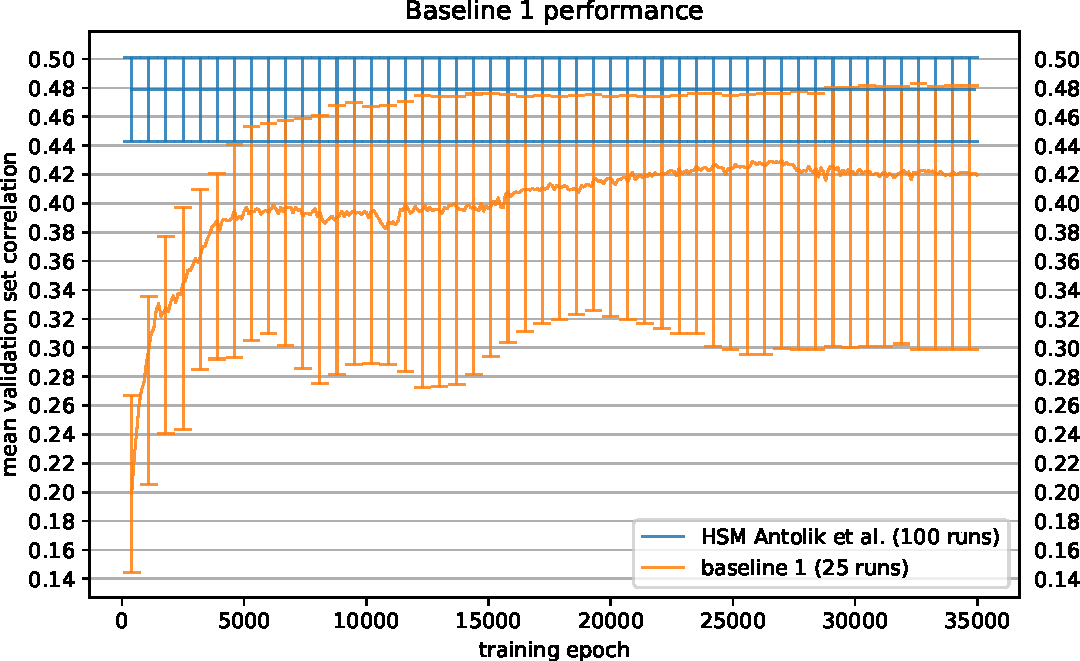
\includegraphics[width=1\textwidth]{../figures/05_1_1_1}
    \caption[Experiment 1.1.1]{Validation set correlation of first \textit{baseline} model versus the original \cite{antolik} implementation\protect\footnotemark on region 1.}
    \label{fig:5.1.1.1}
\end{figure}
\footnotetext{We only have fully trained data for the \citeauthor{antolik} \textit{HSM model}. We thus show the final mean performance and its variance for all time points.}

\subsection{Training hyperparameters tuning}
\subsubsection{Input scaling: Baseline 2}\label{ex:1.2.1}
Informed by the recommended\footnote{\citep{10.5555/645754.668382}} practise of data normalisation, \textbf{experiment 1.2.1} focused on input scaling\footnote{Input scaling has big influence despite the fact that both the first DoG layer and the two subsequent fully connected layers of the model can learn arbitrary linear transformation through the combination of multiplicative weights and additive biases.}. Two different variations were tested. First, where only the input is linearly normalized to have 0 mean and standard deviation of 1. And second, where input is scaled the same way but the output is also scaled to have standard deviation of 1. We could not shift the mean of the output to 0 because that would cause some outputs to be negative and go against our Poisson noise assumption\footnote{Refer to \refsection{ch:1.4.1}.}.

\begin{figure}[H]
    \centering
    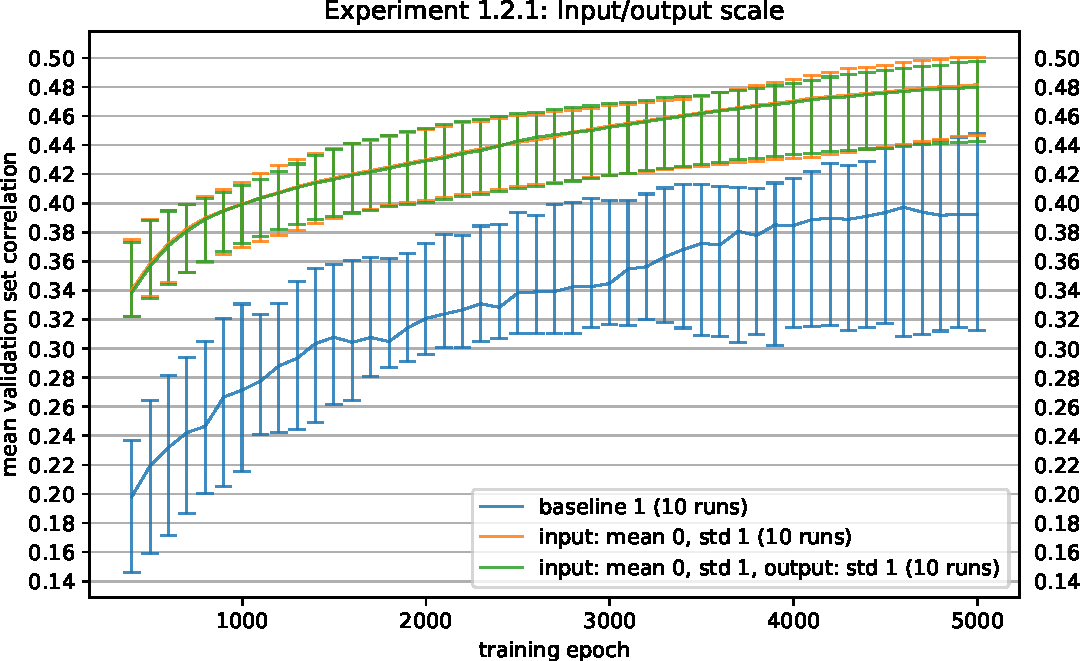
\includegraphics[width=1\textwidth]{../figures/05_1_2_1}
    \caption[Experiment 1.2.1]{Results of \textit{baseline 1} versus normalised inputs\protect\footnotemark.}
    \label{fig:5.1.2.1}
\end{figure}
\footnotetext{Unlike the previous figure \ref{fig:5.1.1.1}, this is restricted to 5 000 epochs and 10 runs per experiment instance. Refer to \refsection{ch:4.4}.}

Figure \ref{fig:5.1.2.1} showcases the dramatic improvement both of these changes had in both 90th percentile run performance but especially stability. Both achieved validation set correlation of approximately 0.48, 0.5, and 0.45 for its median, 90th percentile, and 10th percentile runs respectively after only 5000 epochs\footnote{For experiments we are only training for 5000 epochs (refer to  \refsection{ch:4.4}) and so the performance of the \emph{baseline 1} model is not entirely converged yet.} of training, thus improving over the original \textit{HSM model} by \citeauthor{antolik} Out of the two, we have decided to select the simpler one, scaling only input, as our new base model, \textbf{baseline 2}. Fully trained comparison on 35 000 epochs between \emph{baseline 1} and the new \emph{baseline 2}, achieving 0.51, 0.52, and 0.49 respectively, is presented by figure \ref{fig:5.1.2.1_2}.

\begin{figure}[H]
    \centering
    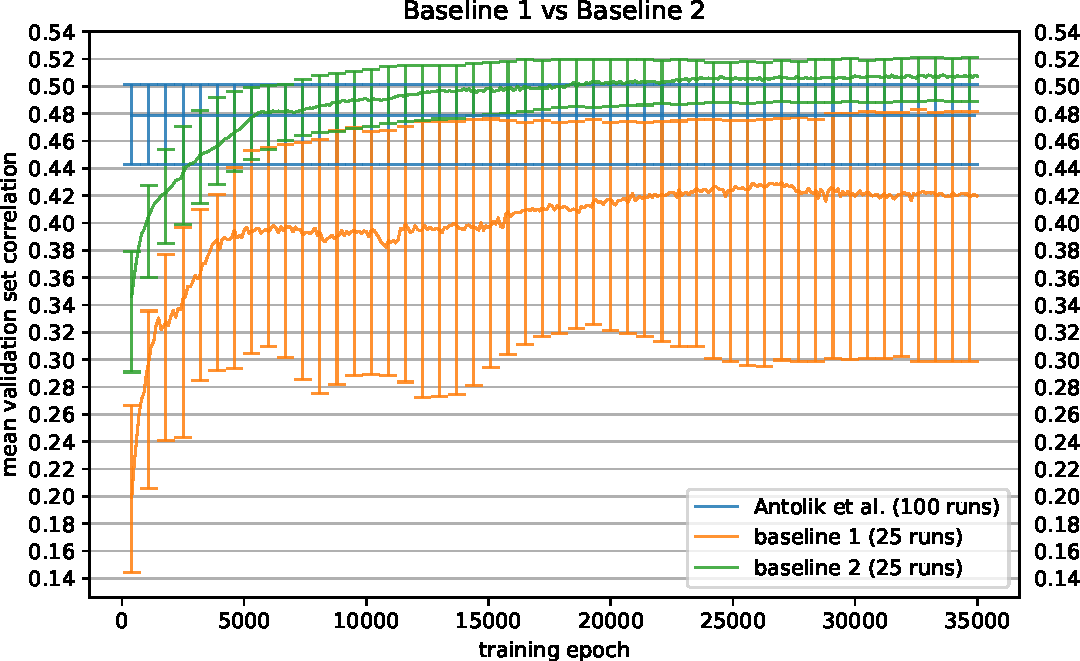
\includegraphics[width=1\textwidth]{../figures/05_1_2_1_2}
    \caption[Experiment 1.2.1 2]{\textit{Baseline 1}, \textit{baseline 2}, and \citeauthor{antolik} implementation\protect\footnotemark[9]. Showcasing the effect of small non-architectural changes.}
    \label{fig:5.1.2.1_2}
\end{figure}

\subsubsection{Gaussian versus Poisson}\label{ex:1.2.2}
The \textbf{experiment 1.2.2}, based on the \emph{baseline 2} model, tested the impact of our assumptions from the \nameref{ch:1.4.1} section in terms of model performance. In line with our expectations and prior research, the version with Gaussian noise assumption loss function had slightly but consistently worse results of (0.46, 0.47, 0.42) after 5 000 epochs of training (Fig. \ref{fig:5.1.2.2}). 

\subsubsection{Bias initialization}\label{ex:1.2.3}

In \textbf{experiment 1.2.3}, we revisited the bias initialization scheme. Instead of the zero initialization chosen for the initial reimplementation\footnote{Refer to \refsection{ch:5.1.0}.} we tested truncated normal initialization\footnote{Refer to \refsection{ch:3.1.1}.} an absolute value of normally distributed samples with 0 mean and 0.1 variance. This was inspired by the presence of strictly positive initialization of biases in the original model. This change proved beneficial (Fig. \ref{fig:5.1.2.2}), yielding a model with generally faster convergence, better median and 10th percentile runs, and only a slightly worse 90th percentile run of (0.48, 0.49, 0.46) after 5 000 epochs of training.

\begin{figure}[H]
    \centering
    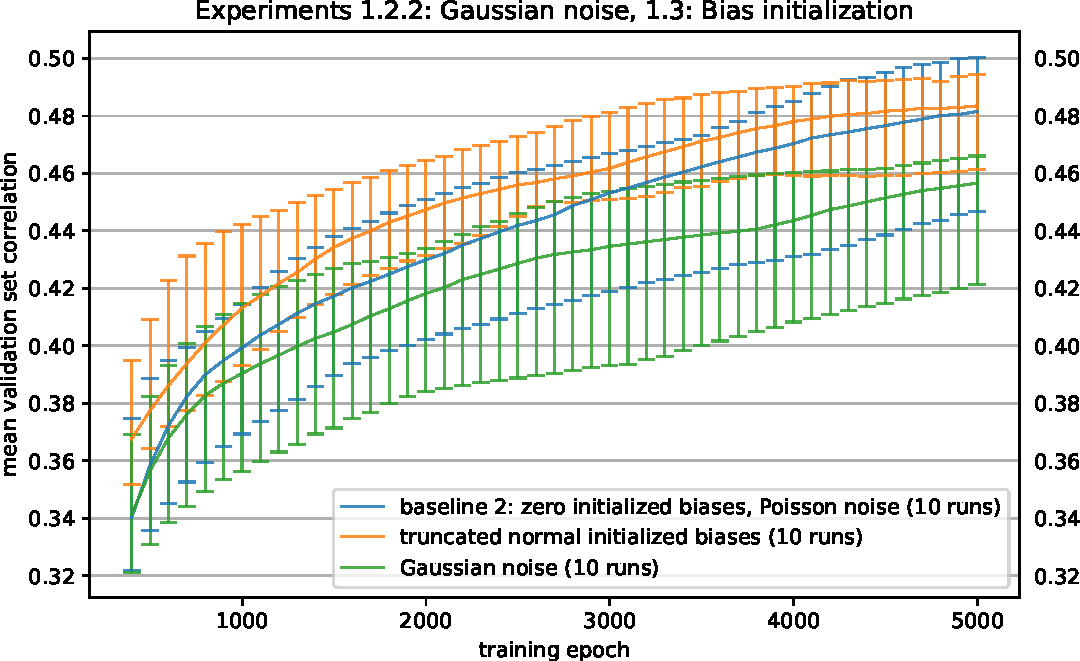
\includegraphics[width=1\textwidth]{../figures/05_1_2_2}
    \caption[Experiments 1.2.2 and 1.2.3]{Impact of gaussian noise and truncated normal initialization of biases (experiments \refexperimentnum{ex:1.2.2} and \refexperimentnum{ex:1.2.3}).}
    \label{fig:5.1.2.2}
\end{figure}

\subsubsection{Learning rate}\label{ex:1.2.4}

The \textbf{experiment 1.2.4} built upon the foundations of our initial experimentation phase\footnote{Refer to \refsection{ch:5.1.0}.} and systematically tested various learning rates for our ADAM optimiser\footnote{While one might assume ADAM should be relatively stable with respect to various learning rates due to its adaptivity based on first and second moments of the gradient, there is little evidence to support this.}. The best performance was achieved by an order of magnitude higher learning rate -- 0.001. It reached correlation of (0.5, 0.51, 0.49) by the end of 5 000 epochs of training (Fig. \ref{fig:5.1.2.4}), substantially increasing overall performance, stability, and also convergence speed over both the previous \textit{baseline} models and the original \textit{HSM model} by \citeauthor{antolik} Further research could be done into dynamic learning rate schedules such as exponential decay rate or step decay. Similarly, both beta and epsilon hyperparameters of ADAM could be explored\footnote{They were kept on their NDN3 defaults for our experiments.} \citep{2019arXiv191005446C}.


\begin{figure}[H]
    \centering
    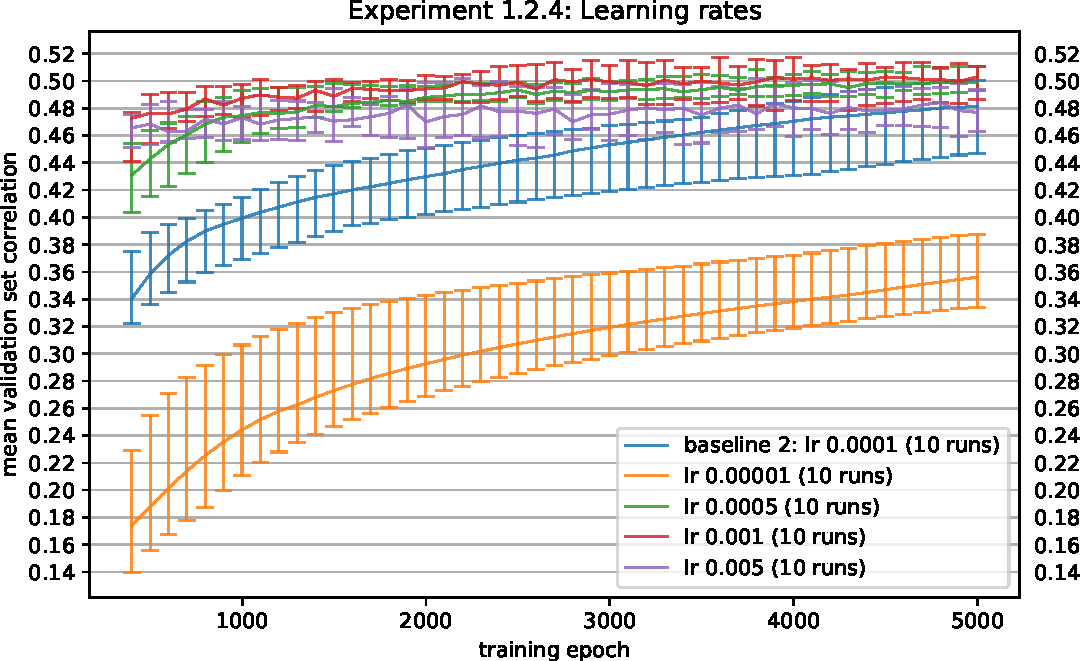
\includegraphics[width=1\textwidth]{../figures/05_1_2_4}
    \caption[Experiment 1.2.4]{Impact of different learning rates.}
    \label{fig:5.1.2.4}
\end{figure}

\subsubsection{Learning rate and bias initialization: Baseline 3}\label{ex:1.2.5}

Combining improvements uncovered by \emph{experiments} \refexperimentnum{ex:1.2.3} and \refexperimentnum{ex:1.2.4}, we created a new base model, \textbf{baseline 3}. Upon training it fully for all 35 000 epochs, we found that the new \textit{baseline 3} converged significantly faster and initially with a substantially smaller spread (figure \ref{fig:5.1.2.5}). 

\begin{figure}[H]
    \centering
    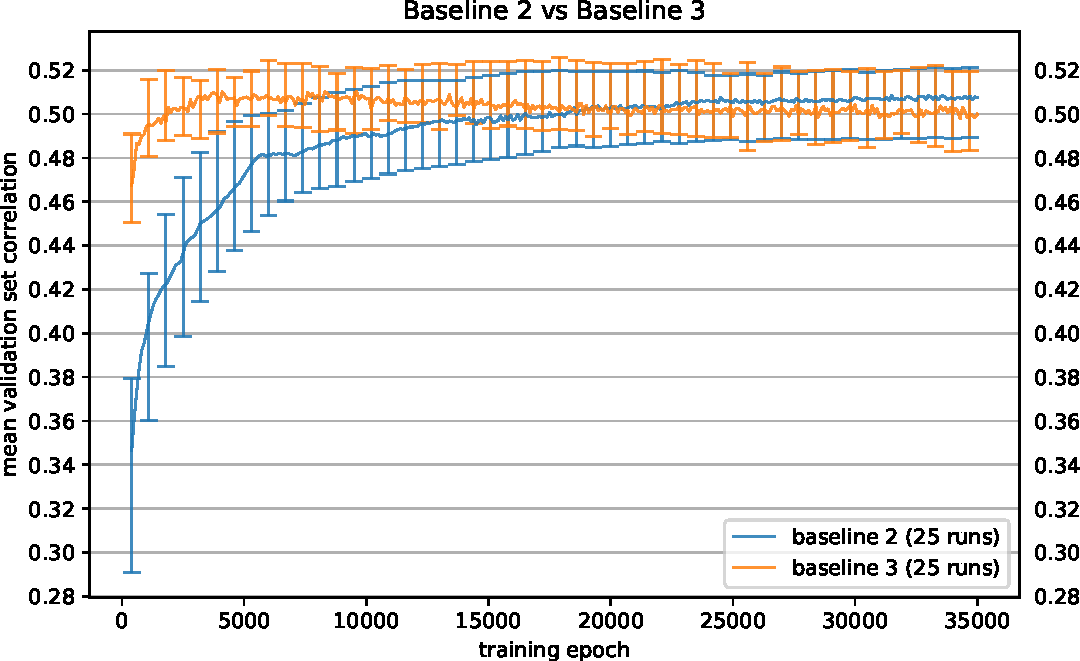
\includegraphics[width=1\textwidth]{../figures/05_1_2_5}
    \caption[Experiment 1.2.5]{Faster convergence, initially smaller spread, and onset of overfitting.}
    \label{fig:5.1.2.5}
\end{figure}

By epoch 6 000 it reached a correlation of (0.507, 0.524, 0.499) versus (0.481, 0.5, 0.454) of \emph{baseline 2} model. Beyond that, however, it started to overfit, eventually falling to (0.5, 0.521, 0.492) versus (0.508, 0.521, 0.49) of \emph{baseline 2} at the end of 35 000 epochs of training. 

Since the peak results were comparable and \emph{baseline 3} showed substantially faster convergence, especially in the 5 000 epochs range -- which is important for experiments evaluation, we chose to use it for all further experiments, replacing \emph{baseline 2}.

\subsubsection{Batch size}

Similarly to \refexperimentnum{ex:1.2.4}, \textbf{experiment 1.2.6} systematically reevaluated another training hyperparameter -- the batch size. To ensure for fair comparison, throughout the experiment we conserved the number of model updates as opposed to the number of epochs\footnote{For more information about the relationship between the number of updates and batch size, please refer to \refsection{ch:1.3.2}.}. I.e. with larger batch size and thus less updates per epoch, we scaled the number of epochs up proportionally. For smaller batch sizes, we did not decrease the number of epochs to ensure each data point is evaluated at least a certain number of times.

\begin{figure}[H]
    \centering
    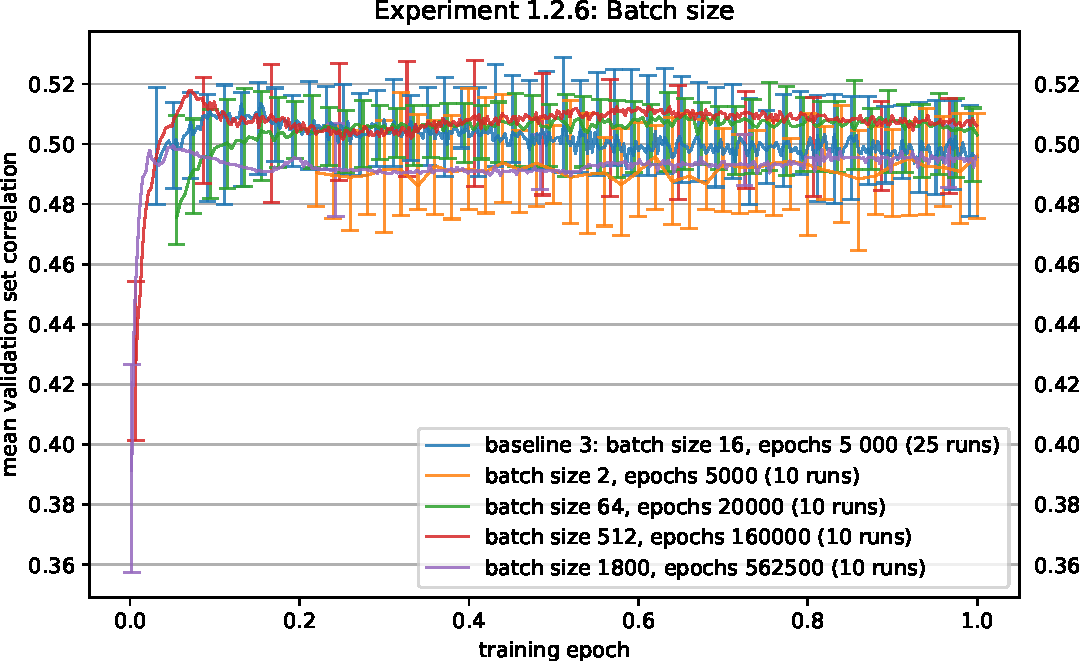
\includegraphics[width=1\textwidth]{../figures/05_1_2_6}
    \caption[Experiment 1.2.6]{Various batch sizes. Training epochs are normalized across instances. 0 being the 0th epoch, 1 corresponding to the last training epoch for that particular instance.}
    \label{fig:5.1.2.6}
\end{figure}

Figure \ref{fig:5.1.2.6} illustrates that batch size had limited impact, with median run performance of all variants between 0.49-0.51 and comparable stability. Both ends of the spectrum, really small batch sizes (2, 4) and the biggest possible (spanning the entire dataset) performed slightly worse than the \textit{baseline 3}. Otherwise, even relatively large batch sizes (512) reached good peak performance\footnote{Even though not unheard of \citep{2017arXiv171100489S}, it is still a relatively surprising result \citep{2017arXiv170508741H}.} and actually proved to be slightly more resilient to overfitting. Due to their computational requirements, however, we chose not to change our training regime for further experiments. The variance in performance between intermediately sized batch (16-128 examples) was not significant enough to draw clear conclusions from.

\subsection{Regularizations and non-linearity}
\subsubsection{Dropout}

\textbf{Experiment 1.3.1} explored dropout\footnote{Refer to \refsection{ch:1.3.2}.} regularization on the hidden fully connected layer. Since dropout can decrease the effective capacity of the model, we tested three sizes of the hidden layer, the original -- 20 \% of the number of output neurons, 30 \% and 40 \%. 

As Figure \ref{fig:5.1.3.1} illustrates, the best result was achieved by the \textit{baseline 3} model without any dropout and with the original hidden layer size. The bigger the dropout, the worse performance. Similarly, for weak or moderate dropout, a larger hidden layer led to lower results. Only for strong dropout (50 \%), a bigger hidden layer outperformed smaller one.

\begin{figure}[H]
    \centering
    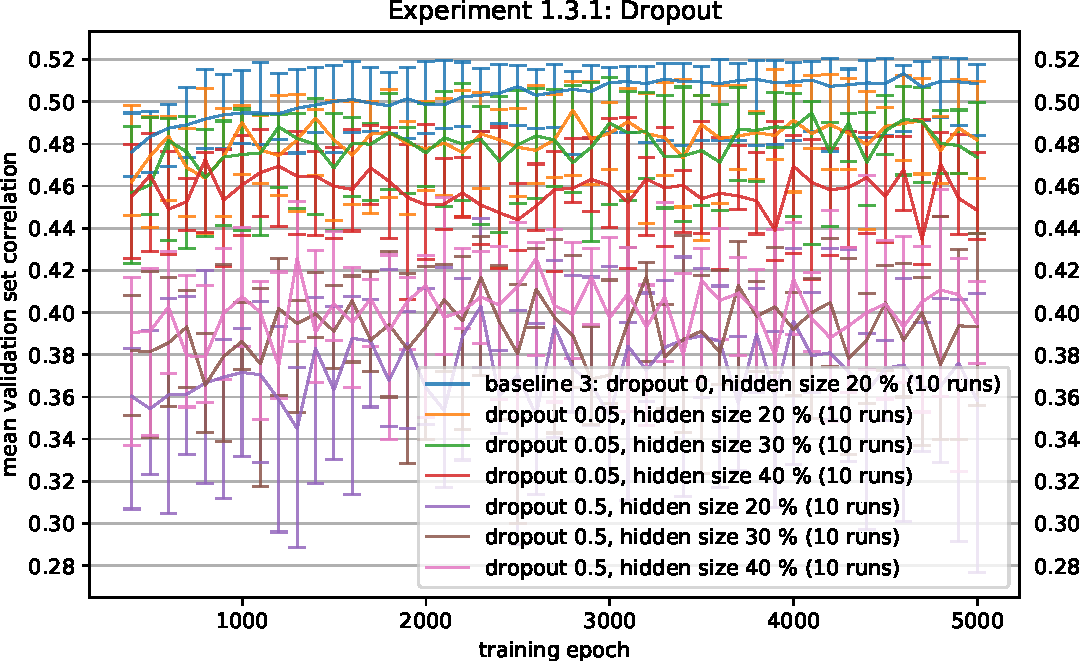
\includegraphics[width=1\textwidth]{../figures/05_1_3_1}
    \caption[Experiment 1.3.1]{Performance loss incurred by dropout regularization (dropout probability) on the hidden layer.}
    \label{fig:5.1.3.1}
\end{figure}

Our working hypothesis for these results is that even light dropout on the hidden layer substantially changes the structure of the network every batch due to the network’s relatively small size. Doing so, it causes significant instability of the gradient and thus disturbs training. This is supported by the observation that the difference in performance cannot be explained just by the smaller capacity of a layer with dropout as this should be more than mitigated by the tested larger variants. The weakest dropout setting drops just one out of the cca. 20 neurons of the hidden layer while the larger variants add cca. 10 and cca. 20 additional neurons respectively. A more thorough exploration would be needed to properly determine the cause, however.

\subsubsection{L1 and L2 regularizations}\label{ex:1.3.2}

\textbf{Experiment 1.3.2} tested L1 and L2 regularizations on both fully connected layers together, the hidden as well as the output, in combination with bigger variants of the hidden layer. The results (Fig. \ref{fig:5.1.3.2}) showed too strong regularization, especially L1 type, effectively prevents training. Moderate L2 mitigated the performance loss induced by a larger hidden layer and seemed to improve convergence speed even for the baseline sized hidden layer variant. L1 led to consistently worse results than L2 for this architecture.

\begin{figure}[H]
    \centering
    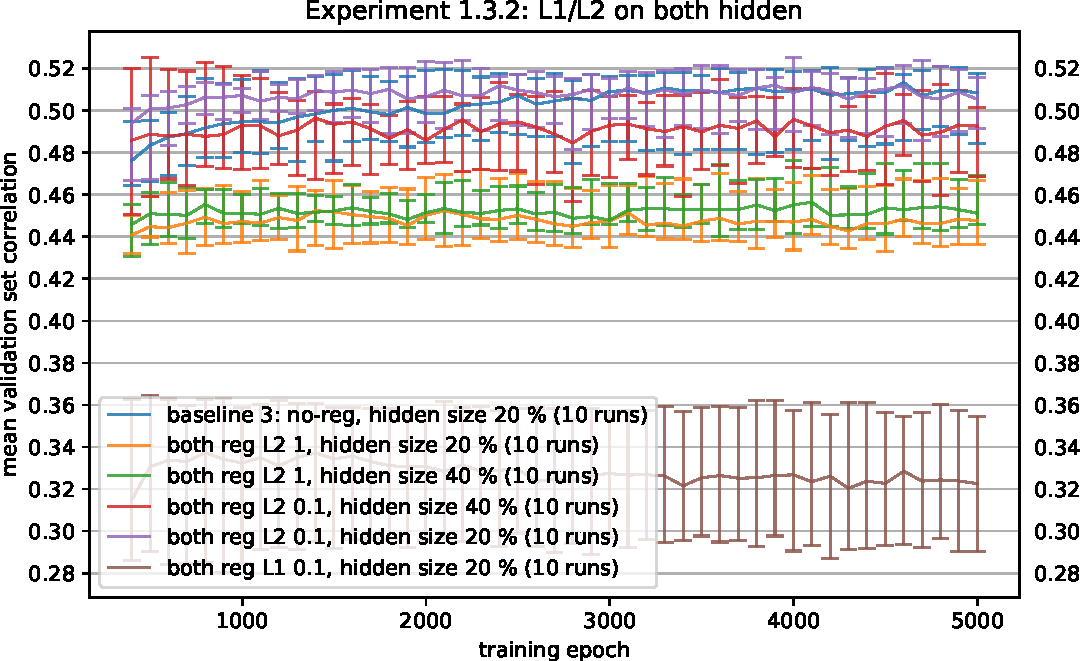
\includegraphics[width=1\textwidth]{../figures/05_1_3_2}
    \caption[Experiment 1.3.2]{Influence of L1 / L2 regularization on both fully connected layers.}
    \label{fig:5.1.3.2}
\end{figure}

\subsubsection{Separate L2 regularizations: Baseline 4}\label{ex:1.3.3}

Informed by \refexperimentnum{ex:1.3.2}, \textbf{experiment 1.3.3}, assessed different strengths of L2 regularization on the hidden and the last layer separately. To fully see the impact on both convergence speed but also overfitting -- to which \textit{baseline 3} model was susceptible to\footnote{Refer to \refexperiment{ex:1.2.5}}, we trained this experiment for full 35 000 epochs.

Figure \ref{fig:5.1.3.3} illustrates that moderate L2 regularization on the output layer leads to better results, especially with longer training during which it mitigates overfitting observed on previous models. The best variant reached an end of training, which was also its peak, performance of (0.513, 0.533, 0.506), improving upon \textit{baseline 3} with (0.496, 0.511, 0.489) end of training and (0.508, 0.519, 0.494) peak\footnote{These numbers do not directly match those reported in \refexperimentnum{ex:1.2.4} because they are computed using only the first 10 runs to enable direct comparison with other experiment instances. Meanwhile, \refexperimentnum{ex:1.2.4} reports numbers from 25 runs as it is a \textit{baselines} comparison.} validation set correlation. We used this instance as the new \textit{baseline 4} model (performance comparison on figure \ref{fig:5.1.5}). Furthermore, any L2 regularization on the hidden layer led to worse performance, regardless of the hidden layer size. At best the benefit of last layer regularization canceled out the drawback of hidden layer regularization, leading to \textit{baseline 3} level of performance.

\begin{figure}[H]
    \centering
    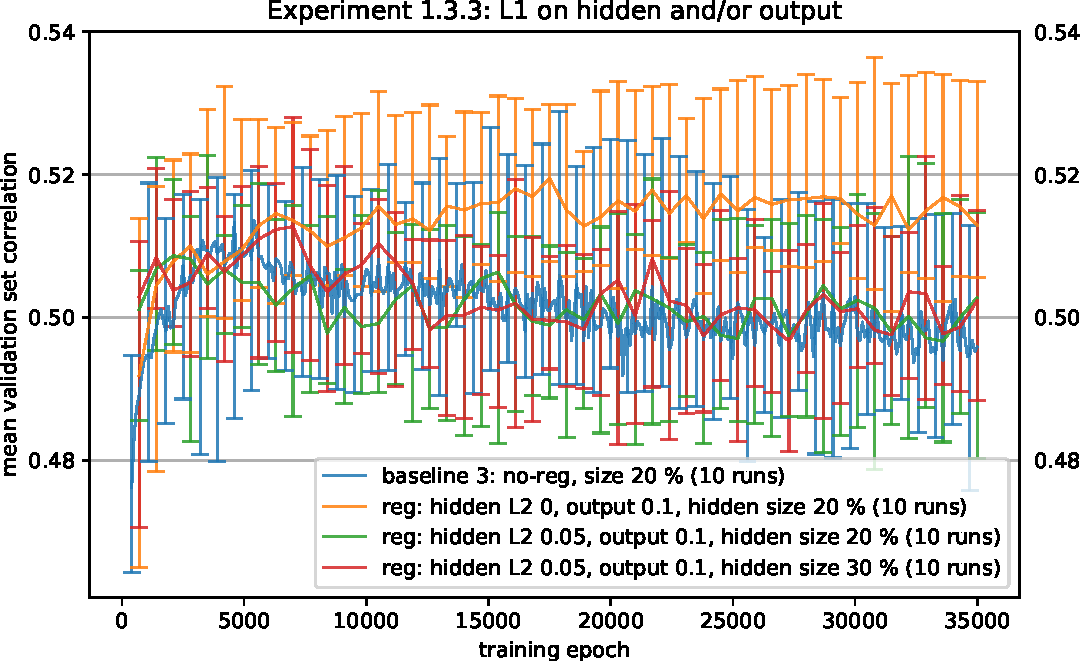
\includegraphics[width=1\textwidth]{../figures/05_1_3_3}
    \caption[Experiment 1.3.3]{Impact of L2 regularization on the output layer with full training.}
    \label{fig:5.1.3.3}
\end{figure}

\subsubsection{DoG layer non-linearity}\label{ex:1.3.4}

\textbf{Experiment 1.3.4} explored adding a nonlinearity after the DoG layer. While the linear activation function of the DoG layer in the HSM architecture by \cite{antolik} is biologically motivated, more recent studies of V1 modeling frequently feature a cascade of convolutional filters, each followed by a non-linearity. For example, \cite{klindt} -- the current state of the art on our dataset, contains 3 convolutional layers and thus 3 non-linearities. Similar architecture can also be seen in \cite{ecker} or \cite{Walke506956}\footnote{More information in \refsection{ch:2.3}.}. The findings of \citeauthor{antolik} proved to be correct, however, with the version containing a SoftPlus nonlinearity after the DoG layer achieving a worse result of (0.494, 0.512, 0.467) versus (0.51, 0.527, 0.502) of \textit{baseline 4} after 5 000 epochs of training.

\subsection{Input scaling}
\subsubsection{Implicit and explicit input scaling}

Intrigued by the results of \refexperimentnum{ex:1.2.1}, \textbf{experiment 1.4.1} systematically tested the impact of input data scaling and the capability of the model to train its own input transformation. We tested 3 ways of preprocessing the data in combination with an automatic, yet explicit, trainable scaling added to the model. The three modes of preprocessing were: the original scale (0-0.000255), our initial scale (0-255), and the -- since \textit{baseline 2} used -- normalisation to 0 mean and 1 standard deviation. Each variant was assessed with and without an additional \textit{linear scale layer}\footnote{Refer to \refsection{ch:3.1.1}.} prepended as the first layer of the model. The experiment was conducted with a \textit{baseline 3} model\footnote{This is a consequence of not presenting the results in the order the experiments were conducted. We, however, believe it does not diminish the significance of the results.}.

The idea behind the \textit{linear scale layer} was that if there was an explicit layer with just two parameters that is only capable of linear transformation of the whole input at once, it should be able to learn any scale relatively easily. Thus achieving close to or exceeding the \textit{baseline} performance, regardless of the input data preprocessing. And if not that, it at least should not lead to worse results as it should be able to stay at its initial parameters, which were initialized to 1 for the multiplicative weight and 0 for the additive bias.

\begin{figure}[H]
    \centering
    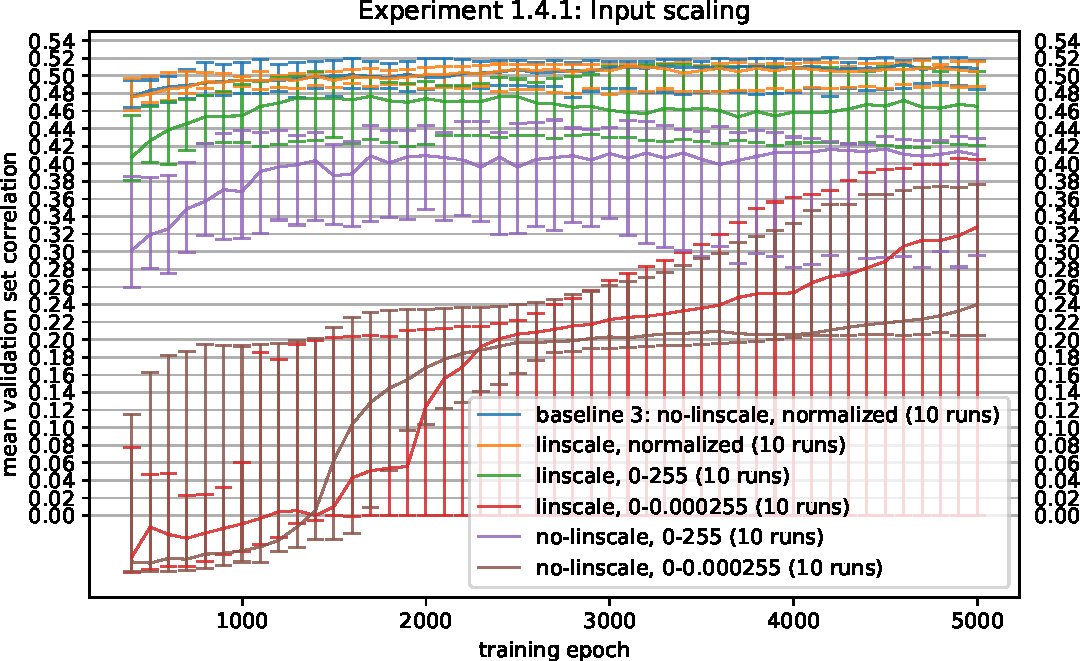
\includegraphics[width=1\textwidth]{../figures/05_1_4_1}
    \caption[Experiment 1.4.1]{Impact of input scaling and explicit \textit{linear scale layer}.}
    \label{fig:5.1.4.1}
\end{figure}

As illustrated by figure \ref{fig:5.1.4.1}, adding an explicit \textit{linear scale layer} improved the results of both \textit{not-normalized versions} of input preprocessing. The \textit{integer variant} (range 0-255) achieved levels of performance higher (0.465, 0.505, 0.421) than its \textit{non-linear-layer-scale-layer} variant (0.41, 0.429, 0.295) but lower than the normalised \textit{baseline} (0.509, 0.517, 0.484). Thus not proving our hypothesis that the \textit{linear scale layer} might effectively learn any transformation -- even the normalisation. Similarly, for the \textit{not pre-processed variant} (0-0.000255), the explicit \textit{linear scale layer} enabled large gains in both 50th and 90th percentile runs but did not improve on the \textit{baseline}\footnote{We are aware that the original scale version with an explicit input scale layer does not show its full potential within the 5 000 epochs of training. There is, however, no reason to believe its peak performance would be substantially higher.}. Notably, its 10th percentile was worse, hinting at the possibility that for extreme distributions of the input data additional free parameters with large effect can lead to unrecoverable training when paired with certain initializations.

For already \textit{normalized input}, both variations with and without the prepended \textit{linear scale layer} fared indistinguishably. That does not mean normalizing is the best possible scale for our data. As shown by this very experiment, our \textit{linear scale layer} achieves sub-par results, and so the absence of a better result with it versus without it does not prove anything. But it at least suggests normalizing might be close to a decent local optimum for our model, an observation in line with literature \citep{Goodfellow-et-al-2016}, \citep{Jin2015}.


\subsection{Discussion}
That concludes the initial set of experiments focused on training hyperparameters, fully connected layers regularization, and generally smaller changes to the original HSM architecture by \citeauthor{antolik}. It showed a few things. First, non-architectural hyperparameters such as learning rate or input data scale can have substantial impact and should always be thoroughly tested. Similarly, a single additional non-linearity can have negative influence despite it being part of related state of the art architectures. 

We also observed that both the median performance and the stability of a model with respect to parameters initializations can differ widely, even for the same or very similar architecture. Through non-architectural changes only\footnote{Adding an L2 regularization on the hidden layer influences only parameters fitting, and so we do not consider it an architectural change in this context.}, we managed to decrease the difference between 90th and 10th percentile runs from 0.18, with \textit{baseline 1} model, to 0.03 of \textit{baseline 4}, while also increasing the median run performance by 0.05 (Fig. \ref{fig:5.1.5}, table \ref{tab:5.1.5}). As a byproduct, this also revealed that analysing a single run with a particular random initialization might paint an incorrect picture. A problem best shown by the 10th percentile run of an \textit{experiment 1.4.1} instance -- that did not train at all while its 50th percentile run fared decently, but by far not limited to only our model or dataset \citep{2019arXiv190910447M}.

\setlength{\abovecaptionskip}{10pt plus 0pt minus 0pt} % Chosen fairly arbitrarily
\begin{table}[H]
    \renewcommand{\arraystretch}{1.0}
    \centering
    \begin{tabular}{l|l|l|l|l|l|l}
        \toprule
        \textbf{Percentile:} & \textbf{50th} & \textbf{90th} & \textbf{10th} & \textbf{50th} & \textbf{90th} & \textbf{10th} \\
        \textbf{Epochs:} & \textbf{5k} & \textbf{5k} & \textbf{5k} & \textbf{35k} & \textbf{35k}& \textbf{35k} \\ \midrule
        Baseline 1 & 0.395 & 0.449 & 0.299 & 0.42 & 0.48 & 0.3 \\ 
        HSM \citeauthor{antolik} & - & - & - & 0.48 & 0.50 & 0.44 \\ 
        Baseline 2 & 0.472 & 0.499 & 0.444 & 0.508 & 0.521 & 0.49 \\ 
        Baseline 3 & 0.507 & 0.517 & 0.498 & 0.5 & 0.521 & 0.492 \\ 
        Baseline 4 & 0.511 & 0.527 & 0.495 & 0.514 & 0.531 & 0.498 \\ \bottomrule
    \end{tabular}
    \caption[Evaluation of 5k/35k epochs training on region 1]{Evaluation set correlation on region 1 across \textit{baseline} models using 25 runs. Performance at epoch 5 000 and 35 000 is shown\protect\footnotemark. }
    \label{tab:5.1.5}
    \renewcommand{\arraystretch}{1.0}
\end{table}
\footnotetext{For the \citeauthor{antolik} model we only have the end of training data.}
\setlength{\abovecaptionskip}{0pt plus 0pt minus 0pt} % Chosen fairly arbitrarily

\begin{figure}[H]
    \centering
    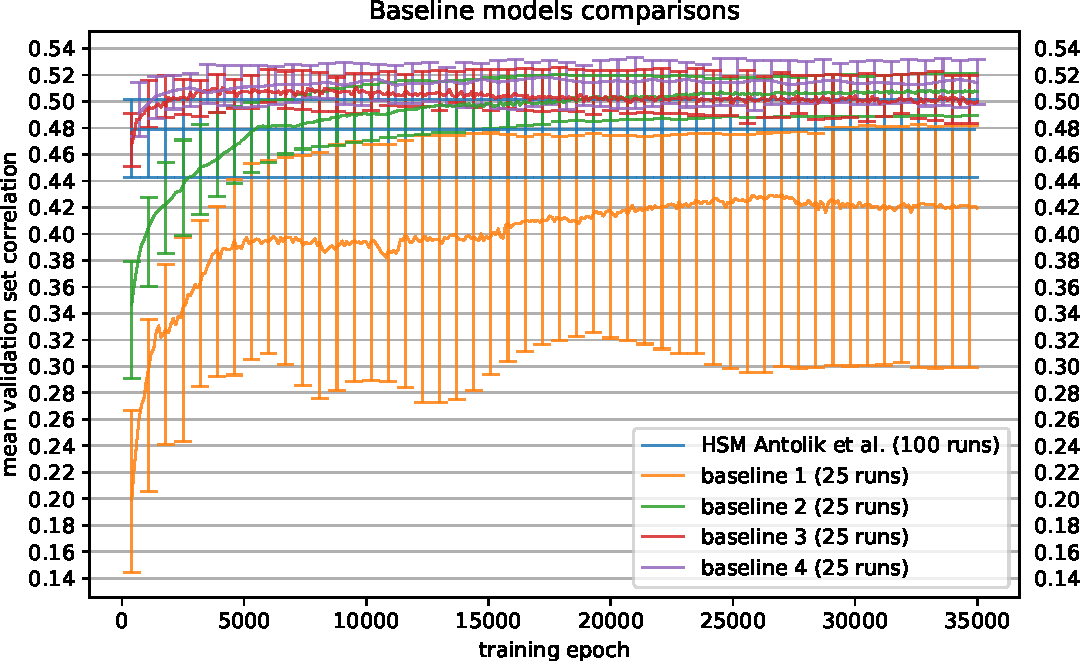
\includegraphics[width=1\textwidth]{../figures/05_1_5_1}
    \caption[Baseline models on region 1]{Evaluation set correlation on region 1 across \textit{baseline} models\protect\footnotemark.}
    \label{fig:5.1.5}
\end{figure}
\footnotetext{We only have fully trained data for the \citeauthor{antolik} \textit{HSM model}. We thus show the final mean performance and its variance for all time points.}

Lastly, we significantly improved convergence speed. While the original model by \citeauthor{antolik} did 1 800 000 000 datapoint evaluations\footnote{100 epochs, each with 10 000 evaluations, using the whole dataset (1800 in case of region 1) batch.}, our model managed with 1/200th of that: 9 000 000, assuming training for 5 000 epochs -- the setting we use to evaluate experiments. If we limited ourselves further, to only 1 000 epochs -- still getting a decent performance of (0.514, 0.531, 0.498) on \textit{baseline 4} model, it would only need 1/1000th of data-point evaluations. While less impressive, our model is better even in terms of the number of model updates -- with requiring roughly half of the original (1 000 000 vs 565 000\footnote{Assuming 5 000 epochs and batch size 16.}) implementation.

\section{Variations on the filter and hidden layers}
In this section, we examine larger architectural changes of the {HSM architecture}, focusing on its first two layers -- \textit{filter} and \textit{hidden}. We compare biologically inspired techniques that feature \textit{hard regularizations} to more generic methods from classical deep learning with \textit{soft regularizations}. We start with fully connected layers, drawing parallels to classical LNLN and LN models, and then move to convolution layer, convolutional variants of the DoG layer, and also the separable layer introduced by \cite{klindt} Unless explicitly specified, all experiments in this section were conducted with a \textit{baseline 4} model.

\subsection{Fully connected models}
\subsubsection{LNLN model}\label{ex:2.1.1}

\textbf{Experiment 2.1.1} explored replacing the first two layers, the DoG filter and the fully connected hidden, with a single fully connected layer. This created an architecture equivalent to an LNLN model\footnote{For more information refer to \refsection{ch:1.2.2}.}. Two fully connected layers, the first serving as a set of filters and the second predicting neural response through per output neuron combination of said filters’ outputs. The same as in an LNLN model, both fully connected layers were followed by a SoftPlus nonlinearity. Inspired by the \textit{hard regularization} properties of the DoG layer\footnote{The resulting difference-of-Gaussians filters are by construction spatially smooth.}, the filter layer featured a Laplacian regularization to ensure spatial smoothness of the filters and the output layer an L2 regularization, as it showed to be beneficial in \refexperiment{ex:1.3.3}.

This experiment was not just to test a completely different architecture. Since the DoG layer in the original HSM architecture is not followed by a non-linearity (Ex. \refexperimentnum{ex:1.3.4}), each output of its second layer is just a linear combination of the results of its first layer’s filters followed by the second layer’s non-linearity. The specific linear combination for each of the second layer’s outputs is dictated by the second layer’s weights. That, however, means we can replace the first two layers of an HSM architecture with a single fully connected layer, whose each filter is an appropriate linear combination (based on the second layer’s weights) of difference-of-Gaussians filters (first layer’s filters). 

While this means, we can construct an LNLN model that can represent any computation the HSM architecture -- and thus our \textit{baseline} models -- can, a question remains whether the biologically inspired \textit{hard regularizations} brought by the DoG layer and the factoring into two separate layers -- filter and hidden -- are not necessary for efficient model training. We tested various strengths of both regularizations in combination with two differently sized sets of filters, 10 \% of the number of output neurons and -- to maintain equivalency with the first two layers of the \textit{HSM model} -- original 20 \%.

\begin{figure}[H]
    \centering
    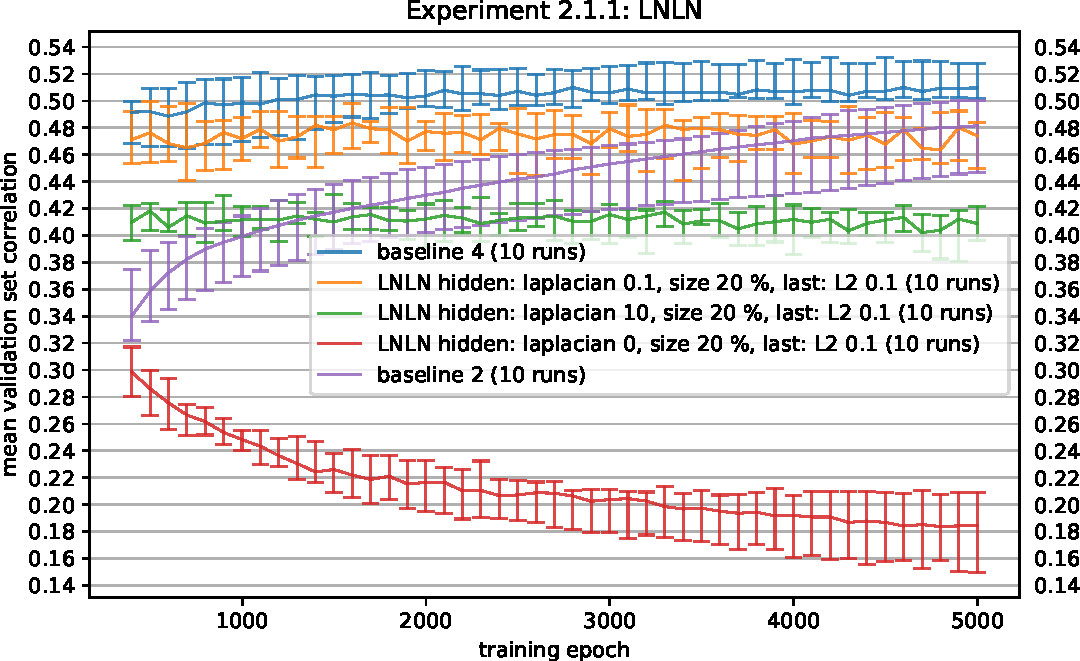
\includegraphics[width=1\textwidth]{../figures/05_2_1_1}
    \caption[Experiment 2.1.1]{Selected LNLN instances versus \textit{baseline 4} and \textit{2}.}
    \label{fig:5.2.1.1}
\end{figure}

The best instance achieved validation set correlation of (0.474, 0.484, 0.45) after 5 000 epochs (Fig. \ref{fig:5.2.1.1}). Despite being worse than \textit{baseline 4} (0.51, 0.527, 0.502), it was comparable to less fine tuned\footnote{While we tried to find optimal hyper-parameters, we did not have enough time to be confident saying this is the best or even close to the best result possible with this architecture. Significantly more time was spent on properly tuning the HSM architecture.} versions of our model, for example the \textit{baseline 2} (0.482, 0.5, 0.447). We believe this result is good evidence for the hypothesis that the biological constraints of {HSM} only serve as well fitting explicit regularizations that make the model more stable with respect to hyperparameters, but are not a necessity to achieve good results. A finding already supported by the state of the art results achieved by \cite{klindt} with a relatively more generic architecture.

A few more noteworthy observations. Moderately strong Laplacian regularization on the hidden layer was paramount. Without it, the model started overfitting very quickly and never recovered. The smaller hidden layer version, with the number of filters equivalent to 10 \% of the number of output neurons, had very similar performance characteristics to the larger version but was worse across the board. Too strong regularization, both on the hidden and the output layer, also caused lower performance.

\subsubsection{LN model}

\textbf{Experiment 2.1.2} tested an architecture equivalent to a simple LN model. The first and only layer featured a spatial Laplacian regularization, with its strength being the only free hyperparameter of the architecture. 

\begin{figure}[H]
    \centering
    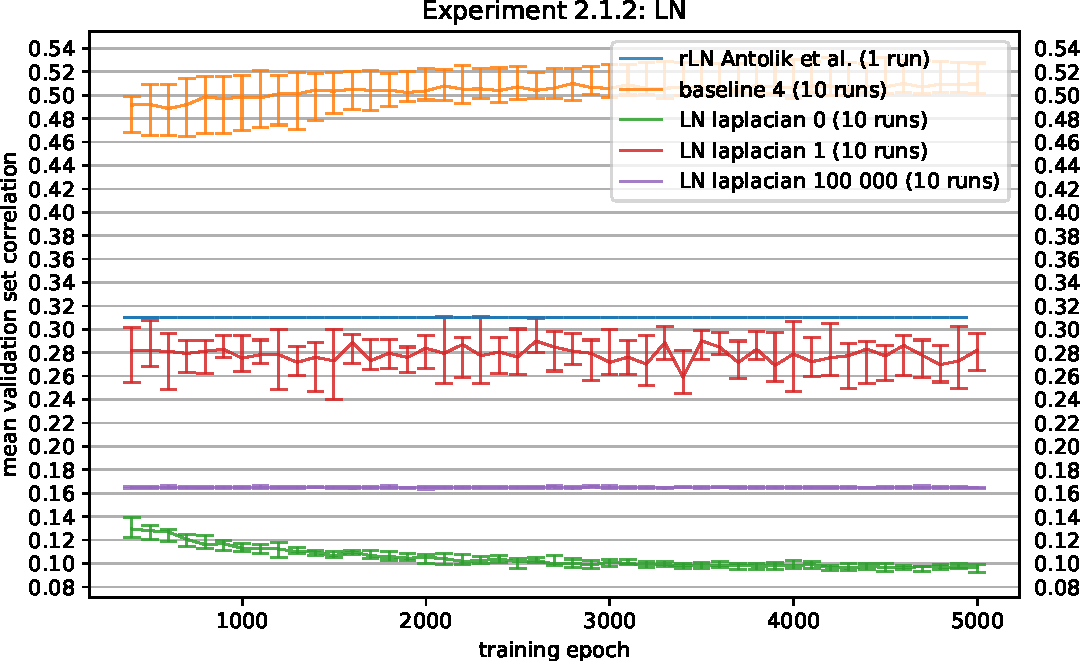
\includegraphics[width=1\textwidth]{../figures/05_2_1_2}
    \caption[Experiment 2.1.2]{Performance of LN-like model instances. Only a fully trained performance is available for the \textit{rLN model} reported by \citeauthor{antolik}\protect\footnotemark.}
    \label{fig:5.2.1.2}
\end{figure}
\footnotetext{We only have fully trained data for the \citeauthor{antolik} \textit{rLN model}. We thus show the final mean performance and its variance for all time points.}

As shown on figure \ref{fig:5.2.1.2}, the results (0.282, 0.296, 0.265) were substantially lower than those of our previously tested and more computationally complex models and on-par with the performance of an analytically optimized version of an \textit{rLN model} with Laplacian regularization reported by \cite{antolik} (0.31). The same as in the previous experiment, some regularization proved to be a necessity while too strong led to poor, albeit very consistent, performance.

\subsection{Convolutional and separable models}
\subsubsection{Convolutions instead of DoG}\label{ex:2.2.1}

In \textbf{experiment 2.2.1}, we replaced the first DoG layer with a normal convolution layer featuring a Laplacian regularization. The rationale was twofold. First, we were inspired by the success of convolution based architectures as reported by \cite{klindt}, \cite{ecker}, \cite{Walke506956}, etc. Given this inspiration, we reintroduced a non-linearity after the convolution layer. Second, much like in \refexperiment{ex:2.1.1} with a fully connected layer, a convolution layer should be able to learn to represent anything the DoG layer can and as such might be viewed as just a more generic and less biologically constrained equivalent. We tested various sizes of the convolution (3 to 15 pixels), numbers of its filters (9 to 30), strengths of the Laplacian regularization, and additional L2 or max\footnote{For details, refer to \refsection{ch:3.1.1}.} regularization of the hidden fully connected layer. Convolution layer stride was set to half of the filter size.

\begin{figure}[H]
    \centering
    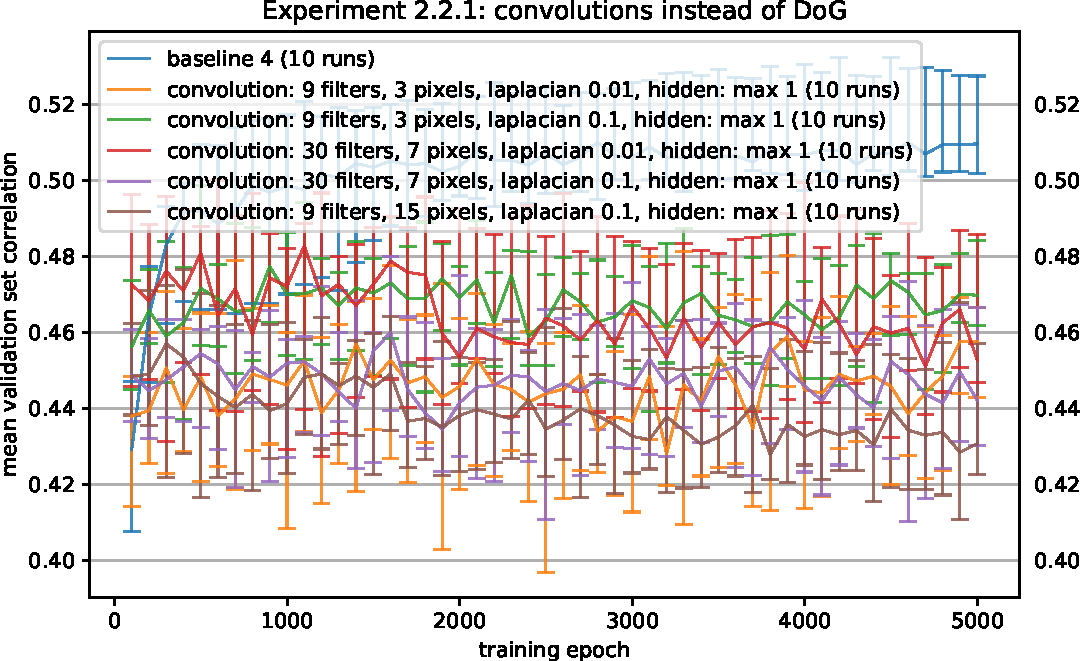
\includegraphics[width=1\textwidth]{../figures/05_2_2_1}
    \caption[Experiment 2.2.1]{Convolution layer with regularization instead of DoG layer.}
    \label{fig:5.2.2.1}
\end{figure}

The results (Fig. \ref{fig:5.2.2.1}) were similar to those of the {LNLN model} experiment (\refexperimentnum{ex:2.1.1}), with the best model achieving validation set correlation of (0.47, 0.484, 0.462) by the end of training. Both instances with 9 filters and 30 fared very similarly. For filter size, both small, 3 pixels wide, and moderate, 7 pixels wide, convolutions reached decent performance, with large filters of 15 pixels being significantly worse (0.431, 0.457, 0.423). Strong max regularization on the hidden layer proved to be a necessity for high performance. In contrast, L2 overwhelmed the training even on the lowest tested strength. 

Some observations were hard to interpret, such as the interaction of Laplacian regularization on the convolution layer and the layer’s filter size. While a stronger variant worked better on a smaller convolution layer with 9 3-pixels wide filters, it worked -- by roughly the same amount -- worse on a larger 7-pixels wide 30 filters instance. A result that is the exact opposite of what we would expect, given the intuition that larger and more numerous filters have more opportunity to overfit and so might require stronger regularization. We hypothesize that, as regularizations in NDN3 are not normalized to layer size, the larger the layer, the higher the chance a regularization on it will overwhelm the loss function and thus negatively impact training. On the other hand, for the largest convolution filters -- 15 pixels wide, stronger Laplacian regularization proved to be beneficial again. A more thorough investigation of this issue would be needed to draw conclusions. At least some Laplacian regularization on the convolution filters was a necessity, however. Without it, the best model reached (0.242, 0.281, 0.209) with clear signs of overfitting.

\subsubsection{Convolutions and separable}\label{ex:2.2.2}

\textbf{Experiment 2.2.2} built on the architecture of \refexperimentnum{ex:2.2.1}, only replacing the hidden fully connected layer with a \textit{separable layer} as it was introduced by \cite{klindt}\footnote{For details, refer to \refsection{ch:2.2}.}$^{,\thinspace}$\footnote{There are still large differences between the \refexperimentnum{ex:2.2.2}'s architecture and \cite{klindt} model. Namely in the number of sequential convolution filters (1 vs 3), absence of batch normalisation, different regularization, and two-layer readout (hidden and output) instead of just a single separable layer.}. This test was motivated by the improvements reported by \citeauthor{klindt} where the separable readout layer increased validation set correlation on region 1 from 0.47 to 0.55 over a fully connected variant. Due to unavailability of max regularization for the separable layer, this test assessed L1 and L2 regularizations for the hidden layer.

These changes led to better results (Fig. \ref{fig:5.2.2.2}), with the best instance reaching peak of (0.494, 0.51, 0.462) and end of training performance of (0.474, 0.499, 0.461). In contrast to the fully connected variant from 2.2.1, small convolution filters had worse performance than larger ones -- with 3-pixels wide being substantially less effective. This was a surprise as we only changed the readout mechanism of the hidden layer and as such did not expect the interactions of the first layer to be different. The number of filters had, as in the previous experiment, little effect.

\begin{figure}[H]
    \centering
    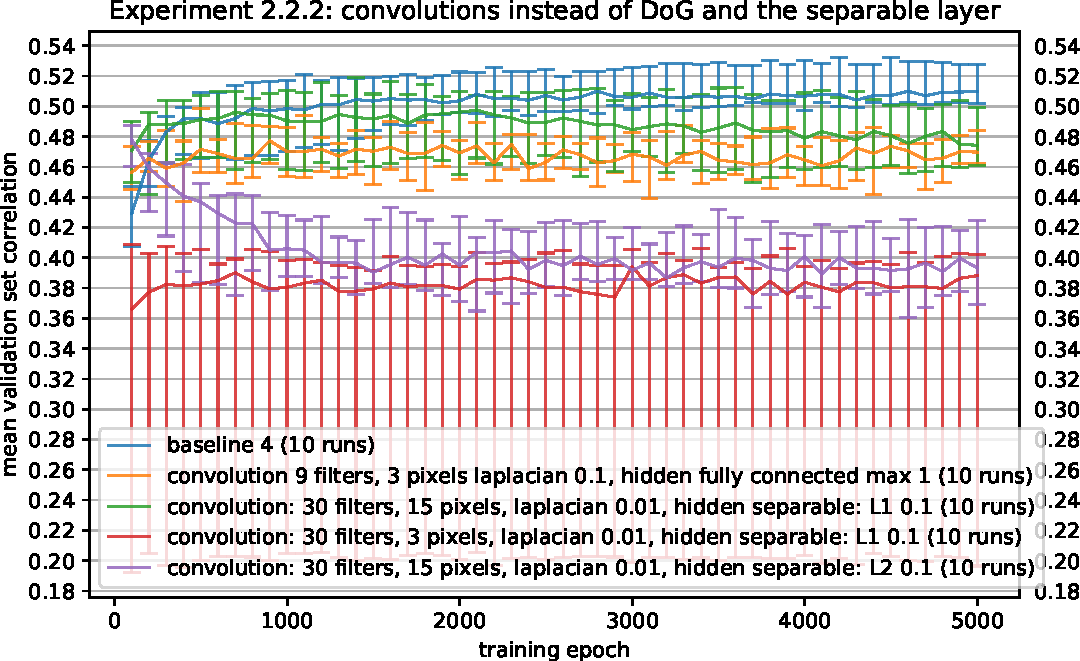
\includegraphics[width=1\textwidth]{../figures/05_2_2_2}
    \caption[Experiment 2.2.2]{Convolution and separable hidden layer.}
    \label{fig:5.2.2.2}
\end{figure}

We also observed another instance (see experiment 2.2.1) of non-additivity of regularization benefits. Moderate L1 on hidden and Laplacian on the convolution worked best, followed by either of them stronger and the other weak, with both of them strong as the least performant variant. L2 regularization on the hidden layer led to significantly worse results across the board.

\subsubsection{Convolutional DoG}

With \textbf{experiment 2.2.3}, we tested two further variants of this architecture. Both featured a convolutional variant of the DoG layer as the first filter layer and had either a fully connected or separable layer as the hidden layer. The tested variants were the same as in \refexperimentnum{ex:2.2.1} and \refexperimentnum{ex:2.2.2} with the obvious lack of Laplacian regularization on the filter layer -- as the convolutional variant of DoG implicitly features a \textit{hard regularization} of its filters.

The rationale behind a convolutional variant of the DoG layer was as follows. Optimizing the locations of centers of difference-of-Gaussians within the DoG layer through gradient descent is not optimal. If the random initialization puts the center completely outside of where it should be, it is unlikely\footnote{Based on our very limited testing of learning properties of the DoG layer. To draw any conclusions, we suggest further research on the interaction between gradient descent based optimizers and the DoG layer.} the gradient for respective location parameters overweights the rest and changes the position substantially\footnote{Fortunately, given the number of filters and size of our input images, this never proved to be an issue on our dataset.}. At the same time, the locational invariance of V1 neurons leveraged through convolution layers by \citeauthor{klindt} and \citeauthor{ecker} should work with explicitly parameterized difference-of-Gaussians filters just as well as with generic filters.

\begin{figure}[H]
    \centering
    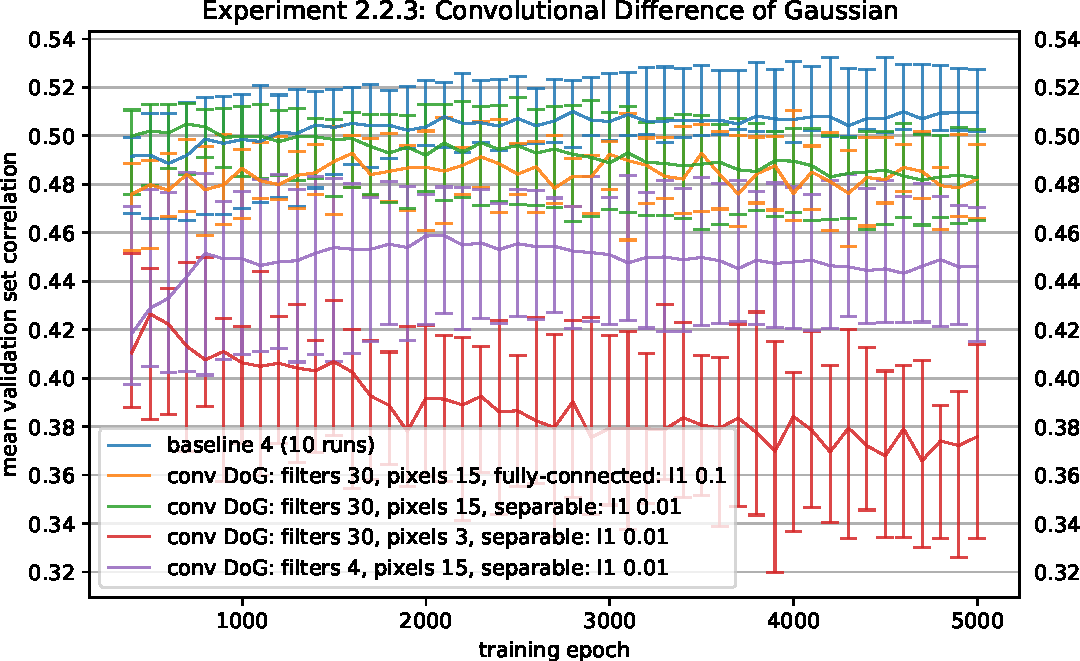
\includegraphics[width=1\textwidth]{../figures/05_2_2_3}
    \caption[Experiment 2.2.3]{Convolutional variants of the DoG layer.}
    \label{fig:5.2.2.3}
\end{figure}

Both versions, with a fully connected as well as a separable hidden layer, achieved a similar level of performance (Fig. \ref{fig:5.2.2.3}), (0.482, 0.496, 0.466) and (0.483, 0.502, 0.465) respectively, that was comparable to a number of recent models such as the convolution variants (\refexperimentnum{ex:2.2.2}). The best instance of the separable version reached a peak of (0.498, 0.51, 0.484) and showed signs of overfitting. For both versions, small 3pixels wide DoG filters did not perform well\footnote{Similar to the {separable version} of {convolutional variant} (\refexperimentnum{ex:2.2.2}) but unlike the {fully connected version} of {convolution variant} (\refexperimentnum{ex:2.2.1}). A plausible explanation is that 3x3 pixels is not enough to fully realize a difference-of-Gaussians filter.}, with the widest 15pixels getting the best results. The number of filters had, as in the previous experiments, relatively low influence with 30 filters achieving initially higher results and then falling, likely due to overfitting.

Notably, the instances with only 4 filters fared substantially worse than their 9 filter counterparts. This was a relatively surprising result. Since 9 filters were enough for a {non-convolutional DoG variant} (\textit{baseline} models), where each filter contains a single difference-of-Gaussians at a specific location, we assumed that the {convolutional variant} that applies each difference-of-Gaussians filter at multiple locations might work with a smaller number of filters. In essence, we assumed that the computation requires a very few types of filters applied at multiple locations instead of a very specific filter for each of relatively few locations. This result, instead, suggests nearby neurons within V1 indeed pool from a rather limited number of LGN inputs that are backed by very specific locations and receptive field topologies within the visual field. We suggest further investigation of the trained weights of this architecture and comparison to the fully connected versions as well as the original HSM version with plain DoG layer.

For the fully connected versions, both L1 and max regularizations worked similarly. The separable version performed best with a light L1 regularization, with L2 overwhelming the training.

\subsubsection{Convolutional DoG without non-linearity}\label{ex:2.2.4}

\textbf{Experiment 2.2.4} investigated the effect of the nonlinearity after the convolutional DoG filter layer on both variants, with a separable as well as fully connected hidden layer. In contrast to convolutional models by others such as those reported by \cite{klindt} or \cite{ecker}, where multiple nonlinearities worked well, for our architecture the variants without a nonlinearity achieved slightly higher results.

\begin{figure}[H]
    \centering
    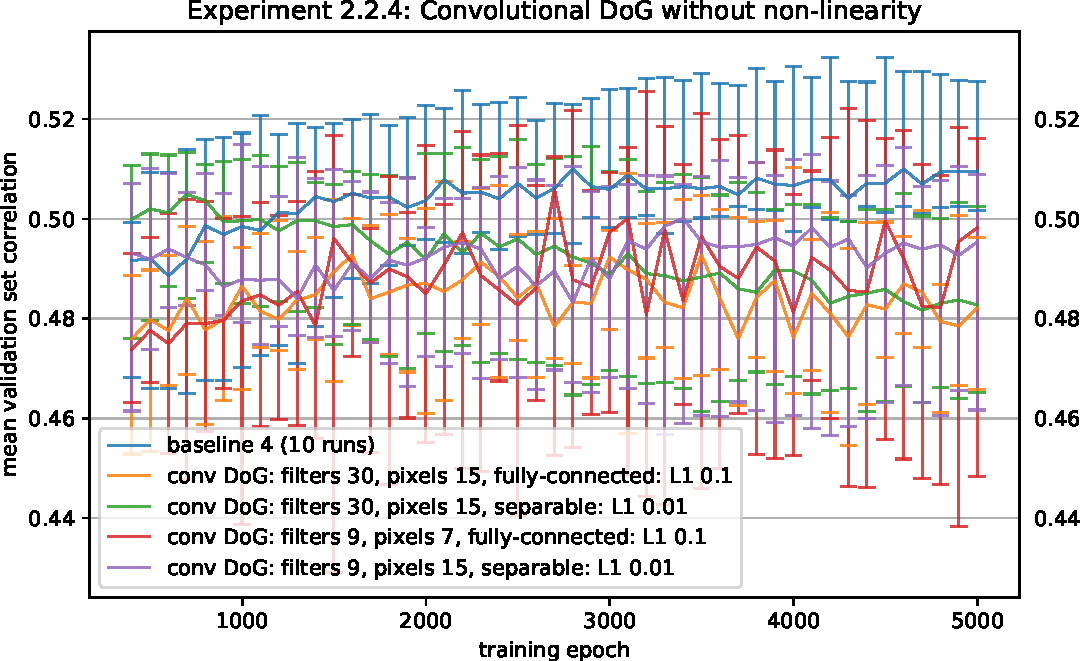
\includegraphics[width=1\textwidth]{../figures/05_2_2_4}
    \caption[Experiment 2.2.4]{Filter layer non-linearity and the convolutional DoG variant.}
    \label{fig:5.2.2.4}
\end{figure}

While still lower than our \textit{baseline} model, the linear version of a fully connected hidden layer variant achieved (0.498, 0.516, 0.448) versus (0.482, 0.496, 0.466) of the nonlinear version (Fig. \ref{fig:5.2.2.4}). And the separable version reached (0.495, 0.509, 0.462) versus (0.483, 0.502, 0.465) of its nonlinear counterpart. Surprisingly, a variant with 7 pixels wide convolutions performed best for the linear activation function version of a separable variant, while 15 pixels filters worked best for all other versions. As in previous experiments, we invite further research into the exact form of the trained filters. Informed by these and \refexperimentnum{ex:1.3.4} results, we also suggest investigating the exact effects of the number of nonlinearities in the model across various architectures.

\subsubsection{Reimplementing what/where model}

Entirely as an exercise, with \textbf{experiment 2.2.5} we tried to reimplement the what/\-where model architecture as introduced by \cite{klindt} Due to it not being the focus of our work, we limited ourselves to only information published in the paper without consulting either of the available implementations\footnote{\href{https://github.com/david-klindt/NIPS2017}{https://github.com/david-klindt/NIPS2017}, \\ \href{https://github.com/aecker/cnn-sys-ident/tree/master/analysis/iclr2019}{https://github.com/aecker/cnn-sys-ident/tree/master/analysis/iclr2019}.}. Given that, we had to grid-search some hyperparameters such as regularization strengths or convolution strides and also chose to use our training regime. 

Further, we replicated the architecture using only techniques already available in NDN3, which forced us to deviate from the original in a number of ways. Instead of the in-NDN3-unavailable group-sparsity regularization on the 3 convolutional layers cascade, we tested max and L2 regularizations. For the same reason, we had to leave out batch normalisation which is originally part of each convolutional layer of the model. Generally, our version was relatively different in terms of things that influence training but was equivalent inference architecture wise.

The best instance reached peak validation set correlation of (0.48, 0.497, 0.461) and (0.479, 0.494, 0.455) at the end of training (Fig. \ref{fig:5.2.2.5}). A result on par with our shallower {convolution variant} of the HSM architecture (experiment 2.2.2) but still below both our \textit{baseline 4} model and especially the published result of 0.55 of the original \citeauthor{klindt} version. As this was a sideline exercise, we did not dedicate further resources to properly reimplement the model. However, we still believe it can serve as evidence that hyperparameters and only training influencing parts of the model can have more substantial impact than larger architectural differences.

In addition to hyperparameters that were in accordance with the paper, we also tested a few other variants. Interestingly, with this architecture L1 regularization worked better than L2 on the output layer. A complete opposite to what we observed on our HSM based models. We also observed that 2-pixel strides on the convolutional layers worked consistently better than half-the-filter-size strides. A result suggesting fine-tuned positioning of first layer filters is important.

\begin{figure}[H]
    \centering
    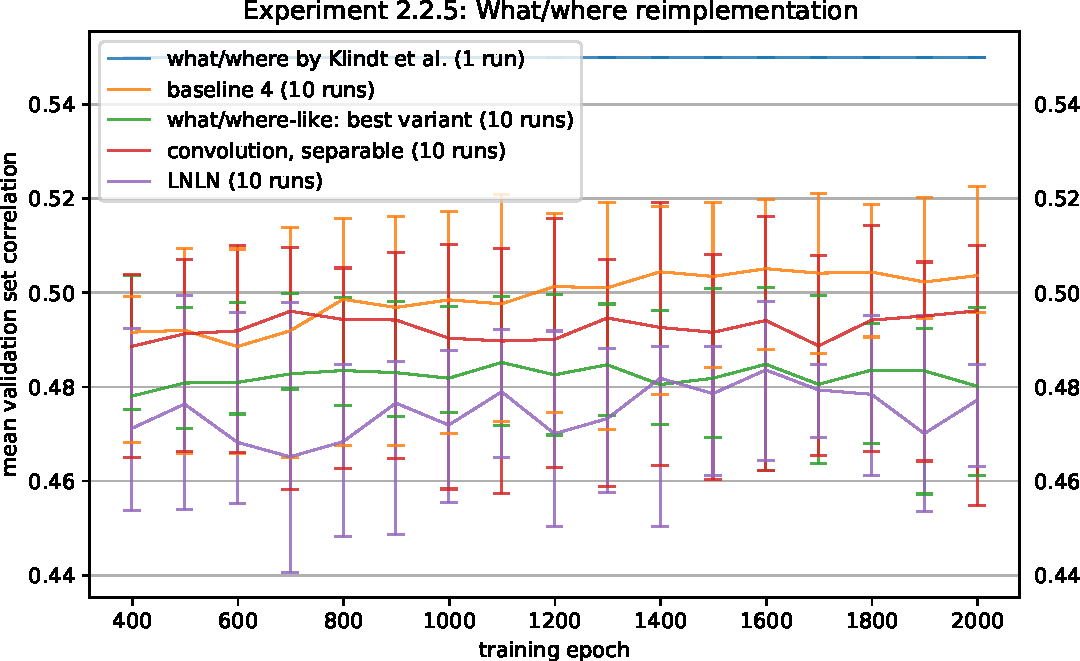
\includegraphics[width=1\textwidth]{../figures/05_2_2_5}
    \caption[Experiment 2.2.5]{Comparing the best reimplemented what/where instance to various other model architectures\protect\footnotemark.}
    \label{fig:5.2.2.5}
\end{figure}
\footnotetext{We only have fully trained data without variance for the \citeauthor{klindt} {what/where model}. We thus show the final mean performance for all time points.}

\subsection{Discussion}

The theme of this section’s experiments could be summarized as testing various computationally more generic architectures. The observed difference between different types of either the first or the second layer was relatively small (Fig. \ref{fig:5.3.2.1_1}). At least when we assumed the best performing instances and in comparison to the variance within one architecture across different hyperparameter combinations. All three versions of the first layer fared very similarly in terms of achieved correlation on the validation set. The {plain DoG variant}, our \textit{baseline}, remained the highest performing. But the difference was so small it could also be explained by not as involved finetuning of hyperparameters for the other variants as was done for the \textit{baseline} models\footnote{Across both the first section experiments and also the original \cite{antolik}}. For this reason, we decided not to test small variations of either of the DoG layers versions, for example with only one Gaussian, a not-concentric version, etc. 

This result was, in a way, expected. All tested alterations are theoretically computationally at least as expressive as the original HSM architecture with plain DoG layer. Its convolutional variant is just a positional relaxation of it, the normal convolutional layer sheds the \textit{hard regularization} constraint on the filter weights, and the LNLN variant just goes one additional step further removing the factoring into two layers. A more surprising observation was that the convergence speed and its progression were also similar. After all, the main difference was that certain variations imposed priors in the form of \textit{hard/soft regularization} on the layers, which we assumed would heavily impact convergence. While a more thorough investigation would be needed, the similar but not better performance of alternatives serves as evidence that the plain difference-of-Gaussians restriction on the first layer filter might be correct but also is not necessary.

\begin{figure}[H]
    \centering
    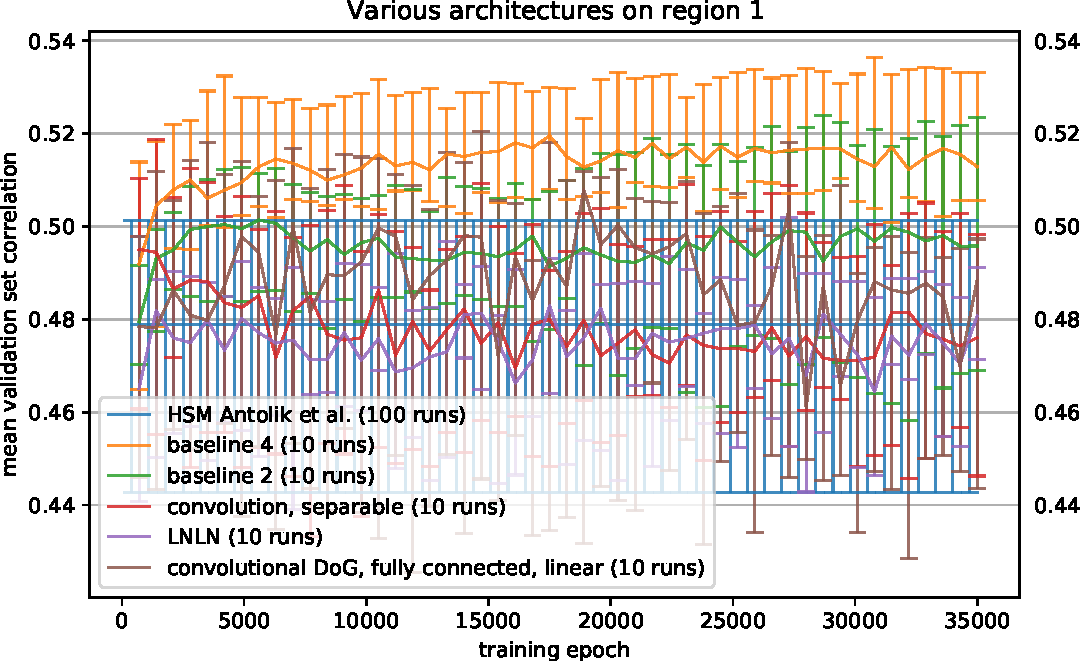
\includegraphics[width=1\textwidth]{../figures/05_3_2_1_1}
    \caption[Various architectures on region 1]{Various architectures\protect\footnotemark fully trained on {region 1}.}
    \label{fig:5.3.2.1_1}
\end{figure}
\footnotetext{We only have fully trained data for the \citeauthor{antolik} \textit{HSM model}. We thus show the final mean performance and its variance for all time points.}


The small observed difference between the variation with a fully connected hidden layer and a variant with a separable layer was also relatively surprising Based on the improvements reported by \cite{klindt} on their architecture, where using it increased the best-achieved performance from 0.47 to 0.55 on region 1, we were surprised by the, in comparison, smaller improvements on our normal convolution variant and almost negligible differences on the convolutional DoG version. It is, however, important to note that there are relatively big architectural differences between those two architectures, such as 1 filter versus 3 filters cascade and an additional fully connected output layer after the readout layer.

Both of the aforementioned results could be further researched. It would be especially interesting to compare the trained weights of the first layer filters and second layer masks between individual variants and figure out if they only lead to comparable levels of performance or if they are, in fact, equivalent computation-wise. Going even deeper, a comprehensive comparison between the \textit{hard regularizations} -- such as the of DoG layer -- and various \textit{soft regularizations} like a Laplacian regularization on a convolutional layer, could also lead to interesting discoveries. 

Similarly, the question of why exactly does adding a non-linearity after the first layer cause diminished performance on our HSM-based architecture but seems to work for deeper models, could also be explored further in at least two ways. First, as a general ML research on the ability of a smaller network to deal with a redundant non-linearity. And second, as a more neuroscience inspired investigation into the question of whether the computation being modeled might actually be as simple as requiring only two non-linearities, with the goal of informing our understanding of visual computation processes.


In agreement with our observations regarding high-level architecture versus hyperparameters tuning and training time details, we also did not manage to achieve published results with our relatively close reimplementation of the what/where model by \citeauthor{klindt} This was mostly due to it being just an afterthought exercise without enough resources allocated to it, but it can, in our opinion, still serve as evidence of the importance of careful tuning. 

We suggest further inquiry in the comparison of multilayer filters, such as those of \citeauthor{klindt} architecture, and single-layer filters of our HSM-based approach. Especially in the face of our aforementioned findings that additional nonlinearity leads to diminished performance in our HSM-based models while the what/where model features a cascade of 3 convolutions, each followed by a non-linearity. 

\section{All regions experiments}

In this section, we make use of all three regions of the dataset\footnote{Refer to \refsection{ch:4.1.1}.}. First, we pool the regions together and test one shared model trained on all data. Second, we assess how various architectures explored in previous sections work on regions 2 and 3 and investigate how well our observations made on region 1 generalize.

\subsection{Combined dataset}\label{ch:5.3.1}
\subsubsection{Region pooled dataset}

\textbf{Experiment 3.1.1} explored pooling multiple regions together to train a single model on higher quantity of data. The rationale behind this was the same as why record and then subsequently fit multiple neurons from a single V1 region at the same time, instead of fitting them one by one separately\footnote{Notably, the LN/rLN model is effectively fitted per neuron.}. While the similarity in both inputs and computational properties is lower between V1 neurons from different regions than within a region, it is still there and -- to a lesser degree -- is even present across neurons from multiple individuals, such as between {regions 1}, {2} and {region 3}. Training one model across data from multiple regions can then help ground the common computation, thus mitigating the effect of random noise that is present in the data, and improve the accuracy of the trained model. All models trained in this experiment were based on \textit{baseline 3}. 

To assess the benefits of this approach, we first needed a baseline model that does not involve any data sharing between regions. We created an ensemble of three separate models, each trained on and responsible for predicting one of the three regions. To measure its performance, we used the average of validation set correlations across the three regions weighted by the number of output neurons in each. Thus, getting an unbiased per neuron average validation set correlation across all available data.

The shared model was trained on all three regions using the data filters capability of NDN3\footnote{Refer to \refsection{ch:3.1.1}}. As such it effectively shared the first two layers, DoG filter and fully connected hidden, between all neurons from all three regions and had per output neuron\footnote{Alternative interpretation is that we are effectively using transfer learning across the tree regions. Pre-training the first two layers of the model on all three regions together and then adding and fine tuning the last layer for each region individually.} -- and thus also per region -- output. Since more data was being fit, the assumption was that the model might need bigger capacity and potentially stronger regularization. To test this, we trained variants with 9 to 25 DoG filters, hidden layer sizes of 20 \% and 30 \% of the number of output neurons\footnote{Across all three regions.}, and various strengths of L2 regularization on both the hidden and the output layers. 

The best instance of the model trained on all three regions pooled together achieved worse performance than its separate-models-ensemble counterpart (Fig. \ref{fig:5.3.1.1_1}), with end of training validation set correlation of (0.439, 0.459, 0.426) versus (0.474, 0.486, 0.46). 

\begin{figure}[H]
    \centering
    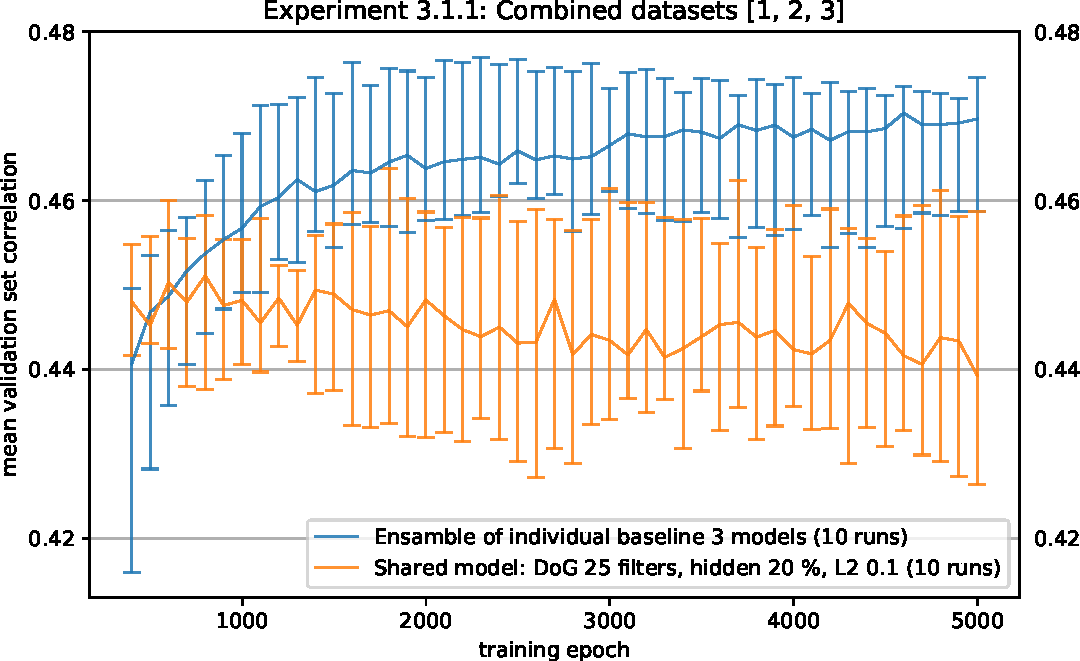
\includegraphics[width=1\textwidth]{../figures/05_3_1_1_1}
    \caption[Experiment 3.1.1]{Models trained on {regions 1,2,3} pooled together\protect\footnotemark.}
    \label{fig:5.3.1.1_1}
\end{figure}
\footnotetext{Shared model represents a single model trained on data pooled together, the ensemble is just a weighted average of three separate models.}

In addition to using all three regions, we also run the same experiment with only the first two regions pooled together, thus limiting ourselves to data recorded from the same animal\footnote{{Regions 1} and {2} were recorded using one animal, {region 3} with another.}. In contrast the three-regions-variant, the model trained on only {regions 1} and {2} pooled together reached correlation of (0.484, 0.495, 0.471), beating (0.475, 0.483, 0.475) of its 2-models-ensemble baseline (Fig. \ref{fig:5.3.1.1_2}).

\begin{figure}[H]
    \centering
    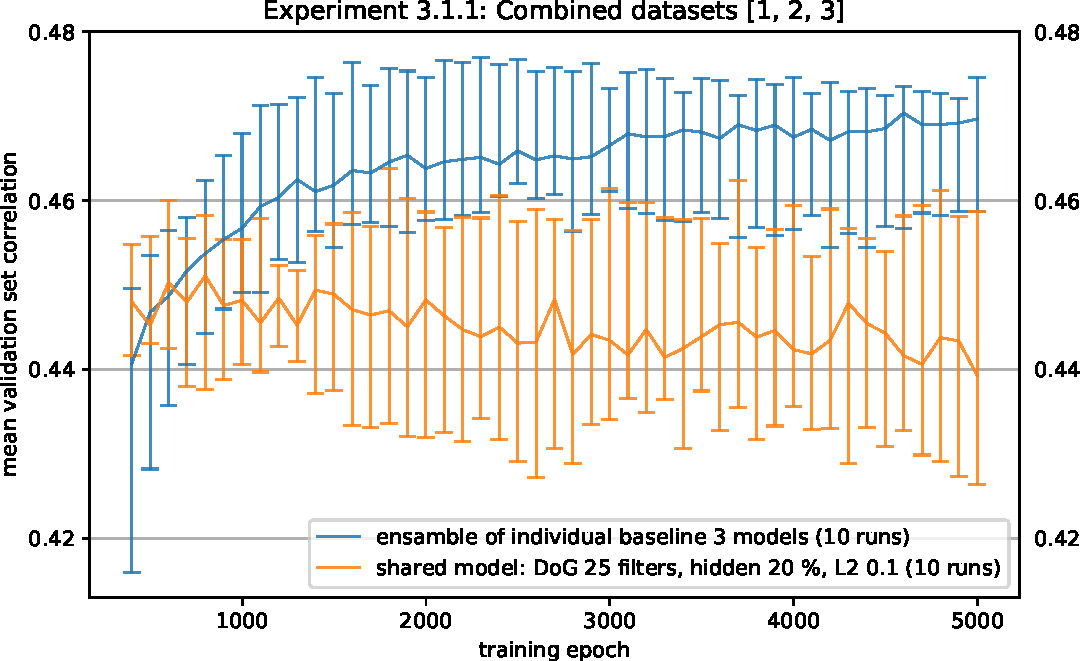
\includegraphics[width=1\textwidth]{../figures/05_3_1_1_2}
    \caption[Experiment 3.1.1 2]{Models trained on {regions 1,2} pooled together\protect\footnotemark.}
    \label{fig:5.3.1.1_2}
\end{figure}
\footnotetext{Shared model represents a single model trained on data pooled together, the ensemble is just a weighted average of two separate models.}

The simplest explanation of this phenomenon would be that the model, when shared across all three regions, did not have enough capacity to handle all the data. Since the hidden layer was proportional to the number of output neurons and we even tested a larger variant -- with worse results, it was unlikely\footnote{It is possible that we might also be experiencing critical regime of deep double descent phenomena \citep{2019arXiv191202292N}.} to be the cause. Similarly, we did not observe differences between variants with 15 and 25 DoG filters that would suggest even more filters were needed. Performance of variants with various levels of L2 regularization on both fully connected layers also did not provide evidence for insufficient regularization. 

With insufficient model capacity and regularization out of the way, several data focused hypotheses explaining these results remained. Notably, the third region was recorded using a different animal and so it is possible the similar computation properties assumption, as declared above, only holds within one animal. Following similar logic, it is possible that the noise distribution across the three regions substantially varies as well. A more thorough exploration would be needed to draw any conclusions, however. Specifically, we suggest further inquiry in the individual region performance of our pooled regions models and a more in depth investigation of the differences between the tree regions data.

A few additional observations. Models trained on pooled regions required more DoG layer filters than the 9 presented in the per-region models, and, with that, benefited from L2 regularization on both the output as well as the hidden fully connected layers. Stronger L2 regularization coupled with only 9 filters led to very poor performance. 

\subsection{Testing on other regions}\label{ch:5.3.2}
\subsubsection{Various architectures across regions}

We finish this chapter with \textbf{experiment 3.2.1} that assessed various architectures from previous sections on each of the three regions. We trained 5 models: \textit{baseline 2} (\refexperimentnum{ex:1.2.1}), \textit{baseline 4} (\refexperimentnum{ex:1.3.3}), the best \textit{LNLN instance} (\refexperimentnum{ex:2.1.1}), the best \textit{convolution instance} (\refexperimentnum{ex:2.2.2}), and the best \textit{convolutional DoG instance} (\refexperimentnum{ex:2.2.4}). Each was trained fully for 35 000 epochs with 10 runs. The motivation was to compare how various architectures fare and if their (relative) performance is stable across different regions

The \textit{baseline} models with plain DoG layer outperformed all other variants across all three regions (Figs: \ref{fig:5.3.2.1_1}, \ref{fig:5.3.2.1_2}, \ref{fig:5.3.2.1_3}, table \ref{tab:5.3.2.1}). However, the improvements of \textit{baseline 4} with respect to both the original reported \citeauthor{antolik} implementation and our \textit{baseline 2} model on {region 1} did not translate to {regions 2} and {3}. Especially on {region 2}, the difference between \textit{baseline 4} (0.414, 0.434, 0.407) and numbers reported by \citeauthor{antolik} (0.412, 0.435, 0.382) was negligible for 90th and 50th percentile, with improvements only in the 10th percentile run. On region 3, the \textit{baseline} models fared better but \textit{baseline 2} model actually outperformed \textit{baseline 4}.

\setlength{\abovecaptionskip}{10pt plus 0pt minus 0pt} % Chosen fairly arbitrarily
\begin{table}[H]
    \renewcommand{\arraystretch}{1.0}
    \centering
    \begin{tabular}{l|l|l|l}
        \toprule
        \textbf{Model} & \textbf{Region 1} & \textbf{Region 2} & \textbf{Region 3} \\ \midrule
        \citeauthor{antolik} & 0.479, 0.501, 0.442 & 0.412, 0.435, 0.382 & 0.437, 0.449, 0.419 \\ 
        Baseline 4 & 0.513, 0.533, 0.506 & 0.414, 0.434, 0.407 & 0.449, 0.455, 0.439 \\ 
        Baseline 2 & 0.496, 0.523, 0.469 & 0.415, 0.429, 0.398 & 0.454, 0.460, 0.449 \\ 
        Convolution & 0.476, 0.498, 0.446 & 0.358, 0.391, 0.306 & 0.416, 0.445, 0.403 \\ 
        LNLN & 0.481, 0.491, 0.471 & 0.340, 0.362, 0.327 & 0.404, 0.417, 0.396 \\ 
        Conv. DoG & 0.486, 0.499, 0.450 & 0.318, 0.363, 0.288 & 0.396, 0.432, 0.384 \\ \bottomrule
    \end{tabular}
    \caption[Performance of various models across regions]{Validation set correlations (50th, 90th, 10th percentiles) of various architectures across three regions.}
    \label{tab:5.3.2.1}
    \renewcommand{\arraystretch}{1.0}
\end{table}
\setlength{\abovecaptionskip}{0pt plus 0pt minus 0pt} % Chosen fairly arbitrarily

While on {region 1} all models, apart from \textit{baseline 4}, fared relatively similarly -- with 50th percentile runs in the range of 0.476-0.496, on {regions 2} and {3} there were two separate groups. With higher performance, there were the variants with plain DoG layer (\textit{baselines 2}, \textit{4}, and the original \textit{HSM model} by \cite{antolik}) and with a significant gap and lower performance all the other architectures (\textit{normal convolution}, \textit{convolutional DoG}, and \textit{LNLN}). The relative performance in the lower group was not stable across regions either, with \textit{convolutional DoG} model performing worst on {region 2} but very comparably to others on {regions 3} and {1}. 

\begin{figure}[H]
    \centering
    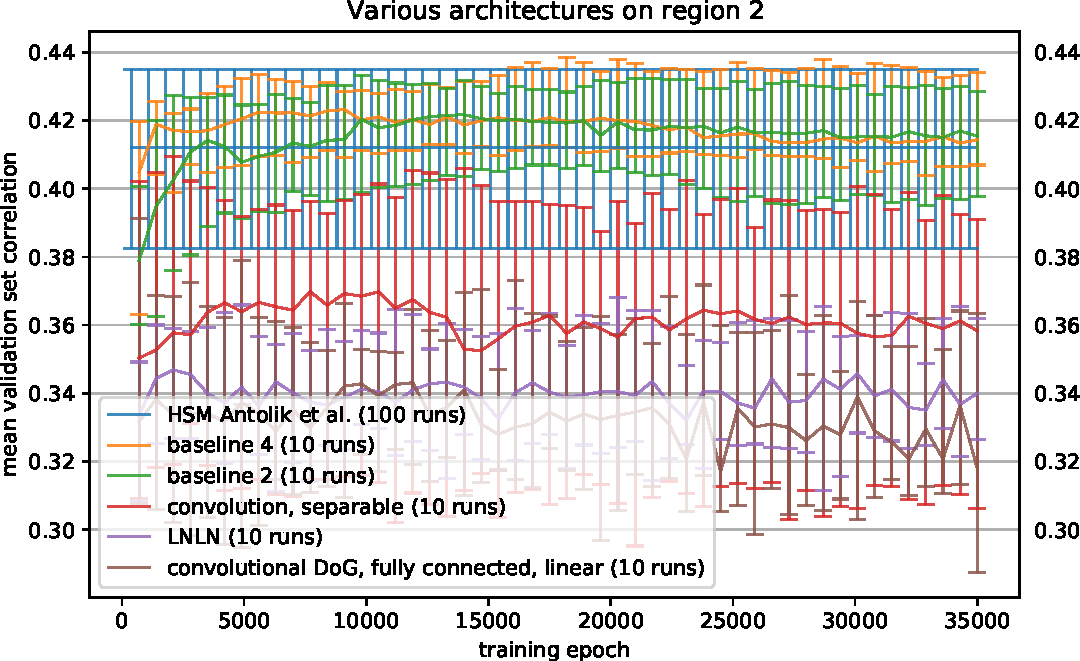
\includegraphics[width=1\textwidth]{../figures/05_3_2_1_2}
    \caption[Various architectures on region 2]{Various architectures\protect\footnotemark trained on {region 2}.}
    \label{fig:5.3.2.1_2}
\end{figure}
\footnotetext{We only have fully trained data for the \citeauthor{antolik} \textit{HSM model}. We thus show the final mean performance and its variance for all time points.}

\begin{figure}[H]
    \centering
    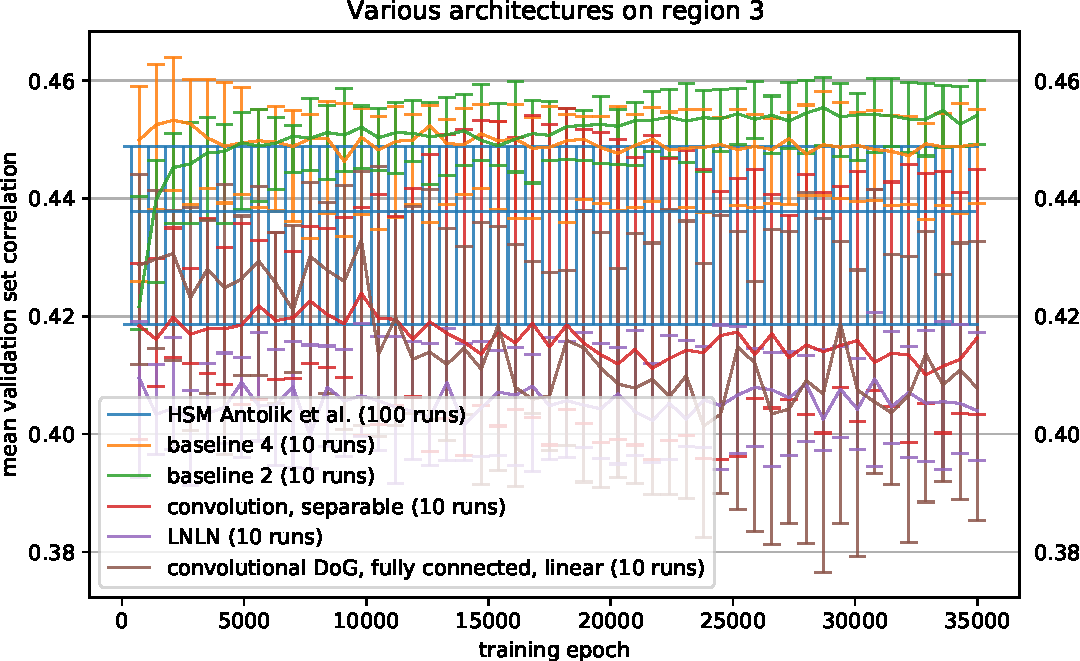
\includegraphics[width=1\textwidth]{../figures/05_3_2_1_3}
    \caption[Various architectures on region 3]{Various architectures\protect\footnotemark[60] trained on {region 3}.}
    \label{fig:5.3.2.1_3}
\end{figure}


The \textit{convolutional variants} (\textit{normal convolution} and \textit{convolutional DoG}) exhibited two noteworthy behaviours. First, they suffered overfitting on {region 3}. This was puzzling since, {region 3} is of the same size as {region 1}, with {region 2} being relatively smaller and thus -- as we would expect -- more susceptible to overfitting. Second, they were significantly less consistent in stability with respect to random initialization across the three regions. This showed especially on {region 2} but was relatively clear even on {region 3}. Surprisingly, the \textit{LNLN model} seemed relatively well behaved in this regard, with its 10-90th percentile run range consistent and comparable to the \textit{plain DoG} variants across all three regions.

Given the big difference between \textit{plain DoG} variants and both of the \textit{convolutional architectures} together with the \textit{LNLN model}, we suspect the main benefit of the \textit{plain DoG} over \textit{convolutional variants}, when it comes to robustness across multiple similar datasets without further fine-tuning, is in the very limited number of outputs from the first filter layer. That said, we were surprised the \textit{separable hidden layer} present in the \textit{convolution model} did not achieve a comparable effect. On similar note, we expected the \textit{hard regularization} of the \textit{convolutional DoG model} or the \textit{location invariant properties} of the \textit{normal convolution model} to also positively influence robustness in comparison to the very generic \textit{LNLN model}. 

A more thorough investigation would be needed to draw any conclusions. We especially recommend looking into the trained weights of each architecture and comparing them across the three regions. Repeating some of the grid-search experiments to fine-tune hyperparameters of the \textit{convolutional architectures} on {regions 2} and {3} might also bring relevant data. For now, however, we believe these results can still serve as evidence for the robustness of the original {HSM architecture} with its plain {non-convolutional DoG layer}.

\subsection{Discussion}

In this section, we made two important findings. First, pooling separately record\-ed regions together to train a single shared model did not provide expected benefits. On the contrary, for the version with all three regions pooled together, it led to worse performance than a simple ensemble of three separate models. To make things more convoluted, this method achieved slightly better results than the ensemble baseline when only the first two regions were pooled. This suggests the intriguing hypothesis that the pooling of the data across regions might work within an animal but not across animals, as {regions 1} and {2} were recorded in the same animal, while {region 3} in a different one. 

Our conclusion is that in our hands, pooling of data across multiple recordings does not impart advantage over fitting models individually. It is, however, important to emphasize that this conclusion is strictly specific to the data available in this thesis and to our current level of understanding of both the dataset and the modeled computation.

Second, we found heterogeneity of outcomes when testing various architectures, fine-tuned on {region 1} in the previous sections, on {regions 2} and {3}. Our improvements of the \textit{HSM architecture} with \textit{baseline} models proved not to be universal, with, for example, \textit{baseline 2} achieving higher than \textit{baseline 4} on {region 3}. We also found that architectures with a {plain DoG layer} were generally more robust when it comes to transferring them to similar, but not equal, datasets without further hyperparameters fine-tuning. In contrast to this finding, we did not observe similar benefit to either the {convolutional DoG} variant or {normal convolution} variant with a {separable readout layer} over a simple {LNLN architecture}.

\setlength{\abovecaptionskip}{10pt plus 0pt minus 0pt} % Chosen fairly arbitrarily
\chapter*{Conclusion}\label{ch:6}
\addcontentsline{toc}{chapter}{Conclusion}
The incorporation of biological detail into deep neural architectures for the purpose of understanding the brain computation is a promising but still only a poorly explored area of computational neuroscience. The HSM model introduced by \cite{antolik}, that was the focus of this thesis, is one such example. While, at the time of writing, outperforming state-of-the-art approaches, the HSM model was implemented in a very ad-hoc fashion, relatively sensitive to initial conditions, and poorly characterized and compared with respect to similar but more traditional DNN architectures. These shortcomings posed a significant barrier for future development of this bio-inspired architecture. The main goal of this thesis was to remedy this situation. 

This thesis offers following contributions:

\begin{itemize}
    \item Reimplementation of the model in modern neuroscience oriented DNN\\ framework.
    \item Identification of hyper-parametrization that improves model’s robustness with respect to initial conditions and input datasets.
    \item Comparison of HSM architecture to more traditional DNNs, showing its advantage - especially especially with respect to robustness.
    \item Evaluation of dataset pooling and model robustness with respect to different regions recording both within the same and across different animals.
\end{itemize}

\section*{Main findings}
\addcontentsline{toc}{section}{Main findings}

The first set of experiments showed us that non-architectural hyperparameters such as learning rate and the scale of input data can have a big impact. Similarly, when those are already tuned, the gains achievable by regularization are relatively minimal - at least for the HSM architecture featuring a plain DoG layer with its hard regularization in the form of explicitly parameterized filters. The second set went further, showing that when properly regularized and fine-tuned, various types of more generic filters (convolution, convolutional DoG, fully connected) work almost identically when used as the first layer instead of DoG layer. Similarly, it failed to show a substantial improvement for variations with a separable hidden layer instead of a fully connected one. It also revealed unexpected interactions with respect to a non-linearity after the first filter layer of the model. 

The third section gave us two insights. First, even though the regions should be similar, improvements made on one do not trivially translate to others. On region 3 we observed a variant of our HSM-based architecture fine-tuned on region 1 perform worse than less tuned versions. Further, we found evidence that even though more generic variants can achieve a similar level of performance as the HSM architecture - with its plain DoG layer, when carefully optimized, they are significantly less robust when used on other regions without hyperparameter changes. Second, pooling regions together and training one shared model does not bring expected benefits, and can actually be detrimental. At least for a variation where all three regions are combined without further processing.

\section*{Lessons learned}
\addcontentsline{toc}{section}{Lessons learned}

Putting it all together, few themes emerge. First, small architectural variations of computationally very similar building blocks are not as significant when best achievable performance is concerned. The biggest difference is in the need for well-tuned regularizations. These are paramount for architectures with higher amounts of free parameters, such as with unrestricted convolution layers or the LNLN variant. With regularization and proper hyperparameters, training to a comparable level of performance similarly quickly is possible, however. 

The benefit of more constrained versions, such as the plain DoG layer variant, is mainly when exhaustive grid search across - not only regularization - hyperparameters is not an option. For example, when we want to use a model fine-tuned on one region on another without further modifications. On this note, the comparable but not better performance of more generic variants of first layer filters (LNLN, convolution) serve as further evidence that the initial part of visual computation might be well approximated using difference-of-Gaussians filters.

Second, the variability of performance with respect to small hyperparameters changes both within a region but mainly across regions can be significant, especially for certain architectures, and the space of all potential hyperparameter combinations is vast. Thus, any conclusions about the underlying fundamentals of the biological computation, that we are trying to model, should be done very carefully. So as not to mistake an observation of one model with a particular set of hyperparameters being better than another one with its set of hyperparameters for a signal about the biological principles of the brain. Similarly, training a set of models per each model instance and analysing distributions of runs instead of single runs proved to be a necessity to even attempt to draw any statistically significant conclusions.

Third, basic deep learning intuition trained mainly on a few types of computer vision problems with vast not-noisy datasets can be helpful but should never be blindly relied upon. As we have seen with the learning rate experiment, explorations of the input data scaling, or additional non-linearity tests, changes that in more standard ML settings might have smaller impact can be relatively influential with this type of data. This ties back to our second lesson learned. Even a significant difference in performance across multiple instantiations of the same model can be due to, for example, the optimizer interacting with a particular data scale better on one architecture than on another and have nothing to do with the similarity between the individual architectures and the computation they are trying to model.

\section*{Future work}
\addcontentsline{toc}{section}{Future work}

As already discussed at various places throughout the \nameref{ch:5} chapter, there are plenty of opportunities for further research. We identified four main areas: further investigation of bigger and computationally non-equivalent architectural changes, analysis of layers activations and the impact of additional non-linearities, comparison of data between regions and proper analysis of models trained on pooled data, and a more involved investigation of the trained weights of both the first layer filters and second layer masks for various architectures already explored in this work.

For further architectures, several options are readily available. Proper reimplementation of the what/where model as introduced by Klindt et al. could be a great starting point that could be followed by exploration of novel deeper architectures, possibly mixing generic convolutions with convolutional and plain DoG layers. Further, we suggest incorporating other layer types in new combinations, such as rotational-equivariant convolutional filters (\cite{ecker}) or, in NDN3 already implemented, separable versions of normal convolutions. Additionally, variants of the HSM architecture with only a single readout layer that is not followed by a fully connected output layer or deeper architectures with less non-linearities could be explored. We also suggest continuing investigating transfer learning with classical computer vision datasets, especially for the initial filter layers. 

Adding batch normalization\footnote{\citep{2015arXiv150203167I}} might also answer some questions - especially around the input scale impact, and potentially unblock deeper architectures. As already discussed in the Experiments and results section, proper investigation into why and how the additional non-linearity on the first filter layer impacts performance could also lead to informative conclusions.

For the third area, we suggest looking at the individual region datasets statistically, and comparing whether they are, in fact, similar in terms of distribution, within region cross-correlations, etc. On the model side, an analysis of what architectures and hyperparameters work on each region, similar to our work on region 1, could also shed some light on the differences between regions. It might also unblock the potential that, we still believe, lies in pooling the three regions and training just one shared model, essentially leveraging within dataset transfer learning. On that note, a good starting point on that might be to test why the combined model had worse performance than the ensemble. Whether it was due to worse performance on only one region or if all regions neurons were negatively impacted by the shared training.

Lastly, an exhaustive comparison of the trained first layer filters and second layer masks of the architectures explored in this thesis could help to unravel the impacts of hard versus soft regularizations. It could answer the question of whether the other first layer variants - that are essentially just more relaxed versions of the DoG layer - converge to it, or if they just achieve a similar level of performance with substantially different filters. Similar inquiry could be done for the hidden readout layer. As part of this, an investigation into how the filters change during training and what is the role of random initialization might also be worth pursuing.


%%% Bibliography
%%% Bibliography (literature used as a source)
%%%
%%% We employ bibTeX to construct the bibliography. It processes
%%% citations in the text (e.g., the \cite{...} macro) and looks up
%%% relevant entries in the bibliography.bib file.
%%%
%%% The \bibliographystyle command selects, which style will be used
%%% for references from the text. The argument in curly brackets is
%%% the name of the corresponding style file (*.bst). Both styles
%%% mentioned in this template are included in LaTeX distributions.

\bibliographystyle{plainnat}    %% Author (year)
% \bibliographystyle{unsrt}     %% [number]

\renewcommand{\bibname}{Bibliography}

%%% Generate the bibliography. Beware that if you cited no works,
%%% the empty list will be omitted completely.

\bibliography{bibliography}

%%% If case you prefer to write the bibliography manually (without bibTeX),
%%% you can use the following. Please follow the ISO 690 standard and
%%% citation conventions of your field of research.

% \begin{thebibliography}{99}
%
% \bibitem{lamport94}
%   {\sc Lamport,} Leslie.
%   \emph{\LaTeX: A Document Preparation System}.
%   2nd edition.
%   Massachusetts: Addison Wesley, 1994.
%   ISBN 0-201-52983-1.
%
% \end{thebibliography}


%%% Figures used in the thesis (consider if this is needed)
\listoffigures

%%% Tables used in the thesis (consider if this is needed)
%%% In mathematical theses, it could be better to move the list of tables to the beginning of the thesis.
\listoftables

%%% Abbreviations used in the thesis, if any, including their explanation
%%% In mathematical theses, it could be better to move the list of abbreviations to the beginning of the thesis.
\chapwithtoc{List of Abbreviations}

\begin{description}
	
	\item[DNN] Deep neural network.
	
	\item[CNN] Convolutional neural network.
	
	\item[NDN3] Neural Deep Network (modeling framework).
	
	\item[LGN] Lateral geniculate body.
	
	\item[V1] Primary visual cortex.
	
	\item[LN] Linear-nonlinear (model).
	
	\item[LNP] Linear-nonlinear Poisson (model).

	\item[rLN] Regularized linear-nonlinear (model).

	\item[GLM] Generalized linear model.

	\item[LNLN] LNLN cascade (model).

	\item[RF] Receptive field.

	\item[STA] Spike Triggered Average.

	\item[MLE] Most likelihood estimation.

	\item[ML] Machine learning.

	\item[DL] Deep learning.

	\item[TF] TensorFlow.

	\item[NP] NumPy.

	\item[DoG] Difference of Gaussians.

	\item[HSM] Hierarchical Structural Model (\citep{antolik}).
	
\end{description}



\chapwithtoc{Glossary}

\begin{description}
	
	\item[Hard regularization]\label{glos:hard-reg} Hard constraint on the computation. For example, in the form of an explicitly parameterized filter that cannot deviate from its form (e.g. difference-of-Gaussians filter instead of an arbitrary fully connected filter). Introduced in \hyperref[intr:hard-reg]{chapter 1}.
	
	\item[Soft regularization]\label{glos:soft-reg} Gradual penalty on certain properties of a computation. Usually implemented as an additional element of the loss function, punishing certain properties of free parameters (e.g. Laplacian regularization on a fully connected filter pushing it towards spatial smoothness). Introduced in \hyperref[intr:soft-reg]{chapter 1}.
	
	\item[Experiment] A single grid-search exploration of a small subset of hyperparameters or architecture aspects.
	
	\item[Experiment instance] One particular model architecture with a specific set of hyperparameters.
	
	\item[Experiment (instance) run] One initialization and fitting of a single experiment instance.
	
	\item[Baseline (model)] An architecture + hyperparameters that is used as a basis for experiments.
	
	\item[HSM / Antolík et al. model] Three layer neural model with DoG layer introduced by \cite{antolik}.

	\item[What/where model] Convolutional neural model with separable layer introduced by \cite{klindt}.

	\item[Receptive field] The portion of sensory space that elicits neuron’s responses when stimulated.

	\item[Readout layer] The first fully connected (or similar) layer after a set of convolutional layers.

\end{description}



%%% Attachments to the master thesis, if any. Each attachment must be
%%% referred to at least once from the text of the thesis. Attachments
%%% are numbered.
%%%
%%% The printed version should preferably contain attachments, which can be
%%% read (additional tables and charts, supplementary text, examples of
%%% program output, etc.). The electronic version is more suited for attachments
%%% which will likely be used in an electronic form rather than read (program
%%% source code, data files, interactive charts, etc.). Electronic attachments
%%% should be uploaded to SIS and optionally also included in the thesis on a~CD/DVD.
%%% Allowed file formats are specified in provision of the rector no. 72/2017.
\appendix
\chapter{Attachments}

\section{First Attachment}

\openright
\end{document}
